\documentclass[11pt]{article}
% Preamble adapted from QCALean's lecture notes, themselves adapted from LinearAQFT's.
\usepackage[a4paper,margin=24mm]{geometry}
\usepackage{amsmath,amssymb,amsthm,mathtools}
\numberwithin{equation}{section}
\usepackage[T1]{fontenc}
\usepackage{lmodern}
\PassOptionsToPackage{dvipsnames}{xcolor}
\usepackage{tikz}
\usetikzlibrary{positioning,arrows.meta,calc,decorations.pathreplacing}
\usepackage{enumitem}
\usepackage{booktabs,longtable,array}
\usepackage{needspace}
\usepackage{placeins}
% Motivating paragraphs; set \motiv to \textcolor{Blue}{#1} to highlight them while vetting.
\newcommand{\motiv}[1]{#1}
\usepackage[hidelinks]{hyperref}
\newtheorem{theorem}{Theorem}[section]
\newtheorem{proposition}[theorem]{Proposition}
\newtheorem{lemma}[theorem]{Lemma}
\newtheorem{corollary}[theorem]{Corollary}
\theoremstyle{definition}
\newtheorem{definition}[theorem]{Definition}
\newtheorem{example}[theorem]{Example}
\theoremstyle{remark}
\newtheorem{remark}[theorem]{Remark}
\theoremstyle{plain}
\newcommand{\R}{\mathbb R}
\newcommand{\C}{\mathbb C}
\newcommand{\Z}{\mathbb Z}
\newcommand{\N}{\mathbb N}
\newcommand{\ii}{\mathrm i}
\newcommand{\cA}{\mathcal A}
\newcommand{\cL}{\mathcal L}
\newcommand{\norm}[1]{\lVert #1\rVert}
\newcommand{\abs}[1]{\lvert #1\rvert}
\DeclareMathOperator{\site}{site}
\newcommand{\comm}[2]{[#1,#2]}
\newcommand{\gcomm}[2]{[#1,#2]_{\pm}}
\newcommand{\ind}[1]{\mathbf 1_{\{#1\}}}
\DeclareMathOperator{\supp}{supp}
\DeclareMathOperator{\dist}{d}
\newcommand{\bd}{\partial}
\DeclareMathOperator{\tr}{tr}
\newcommand{\Mat}{\mathrm M}
\newcommand{\ad}{\mathrm{ad}}
\newcommand{\clock}{\mathsf Z}
\newcommand{\shift}{\mathsf X}

% Passages for the user to vet; set to {#1} once accepted.
\newcommand{\vet}[1]{#1}
\newcommand{\vetnew}[1]{#1}
\newcommand{\reve}[1]{#1}
\newcommand{\vetsource}[1]{#1}
\title{Lieb-Robinson bounds from one theorem}
\author{}
\date{}
% Adapted from QCALean's docs/lecture-notes (commit f7673a2), itself adapted from LinearAQFT's;
% macro prefix QCA renamed LL.
% Navigation only; checked labels are maintained with reviewed correspondence.
\definecolor{LLTagFill}{HTML}{EEEAF8}
\definecolor{LLTagBorder}{HTML}{D6CEEB}
\definecolor{LLTagText}{HTML}{5B477D}
\newcommand{\LLLeanTag}{%
  \tikz[baseline=(tag.base)]\node[rounded corners=1.5pt,
    fill=LLTagFill,draw=LLTagBorder,text=LLTagText,
    line width=0.3pt,inner xsep=3pt,inner ysep=1.5pt] (tag)
    {\normalfont\scriptsize\sffamily Lean\,\ensuremath{\checkmark}};}
\definecolor{LLArtFill}{HTML}{F2F2F2}
\definecolor{LLArtBorder}{HTML}{BDBDBD}
\definecolor{LLArtText}{HTML}{555555}
\newcommand{\LLArtefactTag}{%
  \tikz[baseline=(tag.base)]\node[rounded corners=1.5pt,
    fill=LLArtFill,draw=LLArtBorder,text=LLArtText,dashed,
    line width=0.3pt,inner xsep=3pt,inner ysep=1.5pt] (tag)
    {\normalfont\scriptsize\sffamily formalization};}
\newcommand{\artefact}[1]{#1\nobreak\hspace{0.3em}\LLArtefactTag}
% Status tags for examples without a reviewed Lean counterpart: script ✓ (exhaustively
% verified by a check script) and paper (checked on paper only).
\definecolor{LLScrFill}{HTML}{E8F3EC}
\definecolor{LLScrBorder}{HTML}{BFDCC9}
\definecolor{LLScrText}{HTML}{2F6B45}
\newcommand{\LLScriptTag}{%
  \tikz[baseline=(tag.base)]\node[rounded corners=1.5pt,
    fill=LLScrFill,draw=LLScrBorder,text=LLScrText,
    line width=0.3pt,inner xsep=3pt,inner ysep=1.5pt] (tag)
    {\normalfont\scriptsize\sffamily script\,\ensuremath{\checkmark}};}
\definecolor{LLPapFill}{HTML}{FBF1E3}
\definecolor{LLPapBorder}{HTML}{E6CFA8}
\definecolor{LLPapText}{HTML}{7A5520}
\newcommand{\LLPaperTag}{%
  \tikz[baseline=(tag.base)]\node[rounded corners=1.5pt,
    fill=LLPapFill,draw=LLPapBorder,text=LLPapText,
    line width=0.3pt,inner xsep=3pt,inner ysep=1.5pt] (tag)
    {\normalfont\scriptsize\sffamily paper};}
\makeatletter
\newcommand{\LLExampleStatus}[2]{\expandafter\gdef\csname ll@status@#1\endcsname{#2}}
\newcommand{\LLCheckedLabel}[1]{\expandafter\gdef\csname ll@checked@#1\endcsname{}}
\newcommand{\LLEnableLinks}{%
  \let\LLOriginalLabel\label
  \renewcommand{\label}[1]{%
    \LLOriginalLabel{##1}%
    \ifcsname ll@checked@##1\endcsname
      \nobreak\hspace{0.4em}\hyperlink{lean:##1}{\LLLeanTag}%
    \else\ifcsname ll@status@##1\endcsname
      \nobreak\hspace{0.4em}\LLStatusTag{\csname ll@status@##1\endcsname}%
    \fi\fi}}
\def\ll@script{script}\def\ll@paper{paper}
\newcommand{\LLStatusTag}[1]{\edef\ll@s{#1}%
  \ifx\ll@s\ll@script\LLScriptTag\else\ifx\ll@s\ll@paper\LLPaperTag\fi\fi}
\makeatother

% Labels whose Lean correspondence has been independently reviewed (added after the fidelity
% review of each milestone), and the status of every Example without one.
\LLExampleStatus{ex:twosites}{script}
\LLExampleStatus{ex:twosites-bound}{script}
\LLExampleStatus{ex:chain}{script}
\LLExampleStatus{ex:chainwalk}{paper}
\LLExampleStatus{ex:kernel}{paper}
\LLExampleStatus{ex:cone}{paper}
\LLExampleStatus{ex:twoqubit}{script}
\LLExampleStatus{ex:truncation}{script}
\LLExampleStatus{ex:harmonicchain}{script}
% The one proposition without a Lean counterpart (checked numerically in section 12 of the
% harmonic check script, on one chain; proved on paper).
\LLExampleStatus{prop:rescaling}{paper}
% Marked on 14 Oct 2026 after the independent correspondence review and its re-check of the
% edited statements (58 statements: every theorem-like label with a correspondence entry).
\LLCheckedLabel{prop:commnorm}
\LLCheckedLabel{prop:subfamilies}
\LLCheckedLabel{ex:hamiltonian}
\LLCheckedLabel{prop:pathcount}
\LLCheckedLabel{lem:duhamel}
\LLCheckedLabel{lem:invariance}
\LLCheckedLabel{prop:annihilate}
\LLCheckedLabel{prop:support}
\LLCheckedLabel{prop:first}
\LLCheckedLabel{prop:reset}
\LLCheckedLabel{thm:onestep}
\LLCheckedLabel{thm:iteration}
\LLCheckedLabel{thm:master}
\LLCheckedLabel{prop:walkprops}
\LLCheckedLabel{thm:domination}
\LLCheckedLabel{thm:walkseries}
\LLCheckedLabel{prop:finite}
\LLCheckedLabel{thm:decay}
\LLCheckedLabel{prop:distance}
\LLCheckedLabel{lem:tail}
\LLCheckedLabel{thm:geometry}
\LLCheckedLabel{thm:cone}
\LLCheckedLabel{thm:reverse}
\LLCheckedLabel{prop:derivation}
\LLCheckedLabel{prop:expmul}
\LLCheckedLabel{prop:conjugation}
\LLCheckedLabel{thm:hamgenerators}
\LLCheckedLabel{thm:exchange}
\LLCheckedLabel{lem:glue}
\LLCheckedLabel{prop:localalgebra}
\LLCheckedLabel{thm:quditnet}
\LLCheckedLabel{thm:quditbounds}
\LLCheckedLabel{prop:fnorm}
\LLCheckedLabel{prop:converse}
\LLCheckedLabel{prop:condexp}
\LLCheckedLabel{prop:clockshift}
\LLCheckedLabel{prop:weyl}
\LLCheckedLabel{thm:twirl}
\LLCheckedLabel{prop:bimodule}
\LLCheckedLabel{thm:localapprox}
\LLCheckedLabel{thm:truncated}
\LLCheckedLabel{cor:automaton}
\LLCheckedLabel{prop:lindbladterm}
\LLCheckedLabel{thm:lindbladG1}
\LLCheckedLabel{prop:dephasing}
\LLCheckedLabel{ex:dephasing}
\LLCheckedLabel{prop:bosonicnet}
\LLCheckedLabel{thm:weylcommutator}
\LLCheckedLabel{prop:flow}
\LLCheckedLabel{lem:powers}
\LLCheckedLabel{thm:entrywise}
\LLCheckedLabel{lem:rangerowsum}
\LLCheckedLabel{cor:rangeform}
\LLCheckedLabel{thm:harmonicbound}
\LLCheckedLabel{cor:harmonicclosed}
\LLCheckedLabel{prop:harmonicchain}
\LLCheckedLabel{prop:harmonicwitness}
\LLCheckedLabel{thm:opensystems}

\begin{document}
\LLEnableLinks
\sloppy
\maketitle
\vspace{-2em}
\noindent\motiv{\vet{A Lieb-Robinson bound says that in a lattice of quantum systems with bounded
local interactions, information travels no faster than a finite velocity: the commutator of a
time-evolved observable with a distant one is exponentially small outside a light cone. These
notes are the mathematical account of the Lean library LocalityLean. \vetnew{They prove one
theorem, the path-sum bound: under three hypotheses on the generators of the dynamics, such
commutators are bounded by a sum over paths of overlapping interaction terms. The published
bounds for qudit lattices, open systems and harmonic oscillators are then read off as its
instances; the chapters on fermions and infinite lattices are to come.}}}

{\small\tableofcontents}
\medskip

\section*{About these notes}
\addcontentsline{toc}{section}{About these notes}
\vet{The notes follow the logical build of the theory rather than the order of the literature:
the objects (nets of local algebras, local generators, paths), the central theorem (the path-sum
bound), its closed forms (site matrix, decay functions, light cones), then one chapter per
instance, each showing the same theorem specialized, and finally the thermodynamic limit.

\vetnew{\textbf{Reading conventions.} The numbers in the examples are computed by scripts named in
each chapter's end notes. The literature's terms are used wherever it has one; the terms coined
for these notes are listed below and in the reading guide.}

\vetnew{A statement marked \LLLeanTag{} has a checked proof in LocalityLean or in the libraries
\mbox{LinearAQFT}, \mbox{LocalAlgebrasLean} and \mbox{BosonicLean} on which it builds, whose correspondence with the
statement here has been independently reviewed; the declaration index at the end names the
checked declarations. Every Example, and the one Proposition without a Lean proof (on the rescaling of
units for harmonic bosons), carries exactly one status: \LLLeanTag{} as above,
\LLScriptTag{} when a check script verifies it exhaustively, or \LLPaperTag{} when it is checked
on paper only. Definitions, Remarks and paragraphs of motivation carry no marks.}}

\medskip\noindent\vetnew{\textbf{Coined terms.}} \vet{\emph{Locality in the argument} (hypothesis G1
of Definition~\ref{def:local-generators}); \emph{probe} (the second observable in the commutator)
and \emph{probe reset} (the step of the recursion, Proposition~\ref{prop:reset});
\emph{first-contact path} (Definition~\ref{def:path}); ``a set \emph{crosses} a region'' (it
meets the region and its complement; the sources write the condition without a name);
\emph{site matrix} (the literature's $h_{uv}$, unnamed there); \vetnew{\emph{walk weight}
(Chapter~\ref{sec:closed}: the literature's entries of $h^k$, named for the abstract setting);
\emph{decay function} (the literature's $F$-function, here a function of pairs of sites);
\emph{$F$-bound} (any admissible constant $N_F$ with $h\le N_FF$; the literature's $F$-norm is
the least such).}\par\medskip\noindent \emph{Hamiltonian
family} (Chapter~\ref{sec:qudit}: the literature's interaction, indexed by a finite set so that
one support may carry several terms), ``a matrix \emph{local to} a region'' (the tensor
factor $m\otimes1$, defined by its action on configurations), ``a net with \emph{local
approximation}'' and \emph{$\varepsilon$-local} (Chapter~\ref{sec:approx}: the distance
estimate of the literature's conditional expectation stated as a property of a net, and the
approximate form of the locality condition of a cellular automaton).\par\medskip\noindent The central theorem is called the
\emph{path-sum bound} here, a descriptive name for the content of Theorem~3.4 of
\cite{chen-lucas-yin} and eqs.~(3.41)--(3.42) of \cite{nsy2019}.\par\medskip\noindent \vetnew{Further descriptive
names: the \emph{path series} and the \emph{path count} $P_k(Y,X)$ (the series of the path-sum
bound and its coefficients, the summed weights of the paths of length $k$); the \emph{walk
series}, the \emph{walk bound} and the \emph{walk terms} $\omega_k(t)$ (the same series with the
path count replaced by the walk sums $W_k(Y,X)$, the bound it gives, and its terms,
Chapter~\ref{sec:closed}).\par\medskip\noindent Other descriptive names: the \emph{total strength} (the sum $K$ of the strengths);
\emph{support closure} and \emph{contraction} (the names of hypotheses G2 and G3); the
\emph{commutator seminorm} $N_S(c)$ (the supremum of $\norm{\comm cb}$ over the unit ball of
$\cA(S)$); the \emph{touched sites} (the union $T$ of the supports); the \emph{boundary} $\bd Y$
of a region (its sites touched by a term crossing it); \emph{role exchange} (the bound read
with the observable and the probe interchanged); \emph{contractive negation} (a family whose
negated generators satisfy G3 as well, so that the bounds hold for negative times);
\emph{union-chain} (a sequence of sets each meeting the union of $Y$ and the earlier ones, a
class that fails the comparison with the site matrix); and \emph{distance} for a function $d$
of pairs of sites with $d(u,u)=0$ and the triangle inequality, not assumed symmetric.\par\medskip\noindent For
harmonic bosons (Chapter~\ref{sec:harmonic}): \emph{quadratic generator} (a
Hamiltonian matrix acting on the Weyl labels, the literature's $JM$ transposed), with the
\emph{site matrix} extended to the entrywise absolute value $|K|$ of such a generator, and its
\emph{range} and \emph{row sum}.\par\medskip\noindent Standard
names are kept where the literature has one: Duhamel's identity, Lindblad generator, jump
operator, Pauli matrices, Weyl operators, clock and shift, Heisenberg picture, Banach algebra,
conditional expectation, twirl (the average over a unitary group).} Everything else carries its
name from the sources.}

\section*{Three languages for one bound: a reading guide}
\addcontentsline{toc}{section}{Three languages for one bound: a reading guide}

\noindent\motiv{\vet{Lieb-Robinson bounds are written in two dialects. The review~\cite{chen-lucas-yin}
speaks of a graph whose edges carry Hamiltonian terms $H_e$, of a \emph{site matrix} $h_{uv}$
adding up the strengths of the terms containing two sites, and of walks on the graph; the
mathematical-physics papers~\cite{nachtergaele-sims,nsy2019} speak of an interaction $\Phi$
assigning a self-adjoint term $\Phi(Z)$ to each finite set $Z$ of sites, of a \emph{decay
function} $F$ with a reproducing property, and of the $F$-norm $\norm{\Phi}_F$
(Chapter~\ref{sec:closed} defines the site matrix and the decay functions).

These notes use a third, slightly more general language, chosen so that one theorem covers Hamiltonian and open
dynamics alike: a finite family of \emph{local generators} $L_i$ with supports $S_i$ and
strengths $\kappa_i$, and \emph{paths} of supports from the probe's region to the observable's.
The table says which object plays which role, and where each conversion is proved.}}

\medskip
\noindent\vet{\begin{longtable}{@{}>{\raggedright\arraybackslash}p{0.29\linewidth}>{\raggedright\arraybackslash}p{0.30\linewidth}>{\raggedright\arraybackslash}p{0.35\linewidth}@{}}
\toprule
Review (graph language) & Mathematical physics (interactions) & These notes (generators) \\
\midrule
\endfirsthead
\toprule
Review & Mathematical physics & These notes \\
\midrule
\endhead
edge Hamiltonian $H_e$, $e=\{u,v\}$ & interaction term $\Phi(Z)$, $Z$ a finite set &
generator $L_i$ with support $S_i$; Hamiltonian case $L_i=\ii\comm{\Phi(S_i)}{\cdot}$
(Chapter~\ref{sec:qudit}) \\
strength $\norm{H_e}$ & $\norm{\Phi(Z)}$ & constant $\kappa_i$; equals $\norm{\Phi(S_i)}$ in the
Hamiltonian case; \vetnew{for a Lindblad term the direct strength
$\norm H+\sum_j\norm{\Gamma_j}^2$, by a commutator identity, or $\norm{L_S}$ through the
conditional expectation} (Chapters~\ref{sec:qudit}, \ref{sec:approx}) \\
Heisenberg evolution $e^{\ii tH}Ae^{-\ii tH}$ & $\tau_t(A)$, the automorphism group &
$e^{tL}A$ with $L=\sum_i L_i$; hypotheses G1--G3 (Definition~\ref{def:local-generators}); equal
to the conjugation in the Hamiltonian case (Chapter~\ref{sec:qudit}) \\
operators on the qubits of a region & \vetnew{$\cA_X=\bigotimes_{x\in X}\Mat_n\otimes1$}, the tensor
factor & the matrices local to $X$: zero between configurations differing off $X$, entries
depending on the letters inside $X$ (Chapter~\ref{sec:qudit}) \\
\vetnew{bosons absent} & \vetnew{Weyl operators $W(f)$ with $\tau_t(W(f))=W(f_t)$, the kernel $f_t$ by
normal modes} & \vetnew{a quadratic generator $K$ on the Weyl labels, the flow $T_t=e^{tK}$ and
$\alpha_t(W(f))=W(T_tf)$; the site matrix is $|K|$ (Chapter~\ref{sec:harmonic})} \\
$D(X,Y)$ absent & \vetnew{$D(X,Y)=\min\{\sum_{X\times\bd Y},\sum_{\bd X\times Y}\}$}, eq.~(3.24) of
\cite{nsy2019} & the smaller of the two \vetnew{walk sums or sums of the decay function}, by the role exchange of
automorphisms (Chapter~\ref{sec:qudit}) \\
site matrix $h_{uv}=\sum_{e\ni u,v}\norm{H_e}$, eq.~(3.35) & $\sum_{Z\ni u,v}\norm{\Phi(Z)}\le
\norm{\Phi}_F\,F(\dist(u,v))$, eq.~(3.14) & site matrix $h_{uv}=\sum_{i:\,u,v\in S_i}\kappa_i$, with
diagonal $h_{uu}=\sum_{i:\,u\in S_i}\kappa_i$ (Chapter~\ref{sec:closed}) \\
walk on the graph; irreducible path (Chen--Lucas) & chain of interaction supports with
boundary-crossing sets, eqs.~(3.41)--(3.42) of~\cite{nsy2019} & path: indices $i_1,\dots,i_k$
with $S_{i_1}$ crossing $Y$ and each later support crossing the previous one (no term follows
itself, none is nested in its predecessor), with first contact with $X$ at step $k$
(Definition~\ref{def:path}) \\
\vetnew{$\mathcal C_{X,Y}(t)\le\sum_{x\in X,y\in Y}(e^{2|t|h})_{xy}$}, eq.~(3.36), with
$\mathcal C=\tfrac12\sup\norm{\comm{A(t)}B}$ by its eq.~(3.24) (its (3.22) omits the $\tfrac12$, a
misprint) &
$\norm{\comm{\tau_t(A)}{B}}\le\frac{2\norm A\norm B}{C_F}(e^{2\norm{\Phi}_F C_F t}-1)D(X,Y)$,
Thm.~3.1 of~\cite{nsy2019} & path series (Theorem~\ref{thm:master}), then the two closed forms
as corollaries (Chapter~\ref{sec:closed}); \vetnew{the matrix form is the review's (3.36) with
its constant doubled and the $-1$ that the series proof gives} \\
Haar average over unitaries on $X^c$, Prop.~4.1 & conditional expectation $\mathbb E_X$ as a
finite group average, eq.~(4.6) of~\cite{nsy2018} & conditional expectation $P_X$, the
normalized partial trace, computed as a finite twirl over the Weyl unitaries of $X^c$
(Chapter~\ref{sec:approx}); \vetnew{also a second route to G1 for Lindblad terms, with the
strength $\norm{L_S}$} \\
$\norm{\mathbb E_SA-A}\le\sup\norm{\comm A{B}}\le2\norm{\mathbb E_SA-A}$, Prop.~4.1 & Lemma~4.1 of~\cite{nsy2019} &
local approximation, the same constants (Theorem~\ref{thm:localapprox}); on any causal net the
converse holds for every element of $\cA(X)$ \\
Truncated dynamics $\norm{\tau_t(A)-\tau^{B}_t(A)}$ under the Hamiltonian restricted to $B$,
Prop.~4.3 & --- & $\norm{A(t)-P_{X'}A(t)}$ with the conditional expectation as the local
approximant, a corollary of the walk bound with our constants (Theorem~\ref{thm:truncated});
stated as $\varepsilon$-locality of $e^{tL}$, the approximate form of a cellular automaton's
locality (Corollary~\ref{cor:automaton}) \\
Lindblad generator, Thm.~3.14, with the norms of the terms as strengths & --- & the same
theorem: a Lindblad family is a generator family satisfying G1--G3, G3 as the contraction
hypothesis implied by the review's complete positivity (Chapter~\ref{sec:approx}) \\
--- & CAR algebra, parity automorphism, $\comm{A}{B}=0$ or $\{A,B\}=0$ for disjoint supports,
Prop.~2.1 of~\cite{nsy2018} & graded net; graded bracket $\gcomm{A}{B}$ (Chapter~\ref{sec:fermions}) \\
\bottomrule
\end{longtable}}


\medskip
\noindent\vet{\textbf{Reconnections.} \vetnew{Each chapter from Chapter~\ref{sec:master} on ends
with the sources' statements recovered in the sources' notation: the review's Theorem~3.4 in
Chapter~\ref{sec:master}; Theorem~3.1 of~\cite{nsy2019} in Chapters~\ref{sec:closed}
and~\ref{sec:qudit}; the review's bound for spin systems, its eq.~(3.36), in
Chapter~\ref{sec:qudit}; the review's Theorem~3.14 and Proposition~4.1 in
Chapter~\ref{sec:approx}; Theorem~3.1 of~\cite{nrss2009} in Chapter~\ref{sec:harmonic}; Theorem~3.1
of~\cite{nsy2018} in the chapter to come.} Chapter~\ref{sec:master} sketches the route of the
sources through the Jacobi identity.}


\section*{Notation}
\addcontentsline{toc}{section}{Notation}

\noindent\vetnew{A letter that serves more than one purpose is listed with each use.}

\medskip
\noindent\vet{\begin{longtable}{@{}>{\raggedright\arraybackslash}p{0.26\linewidth}>{\raggedright\arraybackslash}p{0.70\linewidth}@{}}
\toprule
Symbol & Meaning \\
\midrule
\endhead
$\Lambda$ & \vetnew{the set of sites: any set in Chapters~\ref{sec:objects}--\ref{sec:closed} (finite where the matrix form needs it); a finite set in Chapters~\ref{sec:qudit}--\ref{sec:approx}} \\
$X,Y\subseteq\Lambda$ & regions; $X$ carries the observable $a$, $Y$ the probe $b$ \\
$\cA$ & the ambient C*-algebra; $\cA(X)$ the local algebra of $X$ (a net, monotone in $X$) \\
$\comm{a}{b}$ & the commutator $ab-ba$; $\gcomm{a}{b}$ the graded bracket \vetnew{(Chapters~\ref{sec:fermions}--\ref{sec:limit}, to come)} \\
$I$, $i\in I$ & the finite index set of the generator family \\
$S_i\subseteq\Lambda$ & the support of the $i$-th generator, a finite set \\
$L_i$, $L=\sum_i L_i$ & the local generators and their sum, bounded linear maps of $\cA$ \\
$I^{\partial Y}$ & the terms whose support crosses $Y$ (meets $Y$ and its complement) \\
$L^{\partial Y}$, $L'$ & the generator of the crossing terms, and that of the rest, the terms disjoint from $Y$ or inside $Y$ ($L'$ depends on $Y$) \\
$\kappa_i\ge0$, $K=\sum_i\kappa_i$ & the strength of the $i$-th generator (hypothesis G1) and the total strength \\
$J\subseteq I$, $L_J$ & a sub-family of indices and its generator $\sum_{i\in J}L_i$ \\
$N_S(c)$ & the commutator seminorm $\sup\{\norm{\comm cb}:b\in\cA(S),\norm b\le1\}$ of $c\in\cA$ relative to the region $S$ \\
$W,Z\subseteq\Lambda$ & further regions; $Z$ in definitions, $W$ in the support lemma \\
$a,b,c$ & elements of $\cA$: the observable, the probe, and a general element \\
$s$ & an intermediate time, $0\le s\le t$ \\
$A(t)=e^{tL}a$, $B(t)=e^{tL}b$ & the evolved observable and probe, $t\ge0$ in Chapters~\ref{sec:master}--\ref{sec:closed} and all real $t$ for a contractive negation; $e^{\ii tH}ae^{-\ii tH}$ in the Hamiltonian case \\
$f$\vetnew{; $f_0,f_1,f_2$} & an auxiliary function inside a proof; in the sources' route, $f(t)=\comm{\tau_t(A)}{B}$ with the sources' capital letters\vetnew{; the coefficients of the evolved observable in Example~\ref{ex:chain}} \\
$\sigma^x,\sigma^y,\sigma^z$; $\sigma^x_u$ & the Pauli matrices (written out in Chapter~\ref{sec:qudit}); $\sigma^x$ at the site $u$ \\
$C_{X,Y}(t)$ & $\sup\{\norm{\comm{e^{tL}a}{b}}:a\in\cA(X),b\in\cA(Y),\norm a,\norm b\le1\}$ \\
\vetnew{$\ind{P}$} & \vetnew{the indicator of a condition $P$: $1$ if it holds and $0$ otherwise (Chapter~\ref{sec:master})} \\
$\beta_i$ & a continuous majorant of $N_{S_i}(A(s))$ in Theorem~\ref{thm:onestep} \\
$\pi=(i_1,\dots,i_k)$ & a path of length $k$ from $Y$ to $X$; $w(\pi)=\prod_j\kappa_{i_j}$ its weight \\
$P_k(Y,X)$ & $\sum_\pi w(\pi)$ over the paths of length $k$ \\
$\gamma_k(t)$, $B_n(Y,X,t)$ & the coefficient $(2t)^{k+1}/(k+1)!$ and the truncated bound of Theorem~\ref{thm:iteration} \\
\vetnew{$\mathbb B$; $R,Q,G$} & \vetnew{the Banach algebra of Duhamel's identity (a complete normed unital real algebra); elements of it in the identity and its proof} \\
$E,M$ & a Banach space and a closed subspace in the invariance lemma \\
$H$, $\Phi$, $\tau_t$ & a Hamiltonian, the sources' interaction, and their Heisenberg dynamics; in Chapter~\ref{sec:qudit}, $H=\sum_i\Phi_i$ \\
$h=(h_{uu'})$ & the site matrix, $h_{uu'}=\sum_{i:\,u,u'\in S_i}\kappa_i$ (Chapter~\ref{sec:closed}) \\
$T$; $\partial Y$ & the touched sites $\bigcup_iS_i$; the boundary of $Y$, its sites touched by a term crossing $Y$ \\
\vetnew{$\dist(\bd Y,X\cap T)$} & \vetnew{the smallest distance $d(y,x)$ from a site $y$ of the boundary $\bd Y$ to a site $x$ of $X\cap T$ (Chapter~\ref{sec:closed})} \\
$w_k(y,x)$, $W_k(Y,X)$\vetnew{; $w_k(z,X)$} & the walk weights and their sum over $\partial Y\times(X\cap T)$\vetnew{; the sum of $w_k(z,x)$ over $x\in X\cap T$} (Chapter~\ref{sec:closed}) \\
$Q$; $r$ & in Chapter~\ref{sec:closed}: the terms crossing $Y$ and missing $X$; the number of steps a walk needs to reach $X$ \\
$F_0$, $T'$ & a decay function of the distance, and a finite set of sites in the reproducing property \\
$K_1$ & $\sum_i\kappa_i|S_i|$, a bound on the row sums of $h$ \\
$N_F$, $\Sigma_F(Y,X)$ & an $F$-bound of the family ($h\le N_FF$) and the \vetnew{sum of $F$} over $\partial Y\times(X\cap T)$ \\
$g$, $\ell$, $p$, $\rho$ & bounded geometry: terms per site, strength, support size, support diameter \\
$\chi_i(u)$ & the indicator $\ind{u\in S_i}$ of a support \\
$d(u,u')$; $q$ & the distance of a bounded geometry ($d(u,u)=0$ and the triangle inequality); a bound on the row sums of $h$ \\
$\lambda$ & the decay rate of the \vetnew{decay function} in the chain example (Chapter~\ref{sec:closed}) \\
$F$, $C_F$, $\norm{\Phi}_F$ & a decay function, its reproducing constant, the $F$-norm of an
interaction (Chapter~\ref{sec:closed}) \\
$v$, $\mu$ & the velocity $2g\ell p$ of the bounded-geometry bound and the decay rate of the light cone (Chapter~\ref{sec:closed}) \\
\vetnew{$x$, $y$} & \vetnew{sites (Chapters~\ref{sec:closed}--\ref{sec:approx}); $x$ also a nonnegative real in Lemma~\ref{lem:tail} and the proof of Theorem~\ref{thm:cone}; in the first half of Chapter~\ref{sec:qudit} also elements of $\cA$, in $\mathrm L_x$, $\mathrm R_y$, $\ad_x$} \\
$\mathrm L_x$, $\mathrm R_x$ & the left and right multiplications by $x$ (Chapter~\ref{sec:qudit}) \\
$\ad_x$ & the derivation $a\mapsto\ii\comm xa$ \\
$\Phi_i$, $H_J$, $U_t$ & the terms of a Hamiltonian family, the Hamiltonian of a sub-family, and the unitary $e^{\ii tH}$ \\
$\Omega_u$, $\Omega$; $n$ & the alphabet at the site $u$, a uniform alphabet; the dimension of a qudit, $\Omega_u=\{0,\dots,n-1\}$ ($n$ is also the length of a chain in the examples) \\
$s$, $s\sim_Xs'$, $s|_X$ & a configuration; agreement off $X$; the restriction to $X$ \\
\vetnew{$r$, $r'$} & \vetnew{configurations, in Chapter~\ref{sec:qudit}} \\
\vetnew{$M$, $N$} & \vetnew{matrices of the qudit algebra (Chapters~\ref{sec:qudit}--\ref{sec:approx})} \\
\vetnew{$m$; $m_i$} & \vetnew{a matrix on the letters of a region; the matrices of a qudit interaction (Chapter~\ref{sec:qudit})} \\
$\xi$, $\eta$; $(\xi,s|_{X^c})$ & choices of letters on a region ($X$ in Chapter~\ref{sec:qudit}, the complement $Y=X^c$ in Chapter~\ref{sec:approx}); the configuration with the letters $\xi$ on $X$ and those of $s$ off $X$ \\
\vetnew{$(s|_X,\eta)$} & \vetnew{the configuration with the letters of $s$ on $X$ and $\eta$ off $X$ (Chapter~\ref{sec:approx})} \\
$l$, $l'$ & letters of one cyclic alphabet $\Z_n$, indexing the clock and shift matrices and the character sum (Chapter~\ref{sec:approx}) \\
\vetnew{$q_u$} & \vetnew{the order of the cyclic alphabet $\Omega_u=\Z_{q_u}$ at the site $u$ (Chapter~\ref{sec:approx})} \\
$\omega_k(t)$ & the walk term $(2t)^{k+1}W_{k+1}(Y,X)/(k+1)!$ \vetnew{of the pair $(Y,X)$, $k\ge0$ (Chapter~\ref{sec:closed}, used in Chapter~\ref{sec:approx})} \\
$\zeta$; $\Theta$ & re-indexed letters in the twirl proof; the conjugation $a\mapsto\Gamma a\Gamma$ of the dephasing proof (Chapter~\ref{sec:approx}) \\
$\alpha$; $D(X,Y)$ & the exponent of the \vetnew{polynomial decay function $F_0(r)=(1+r)^{-\alpha}$}; the smaller of the two boundary sums in the sources' bound (Chapter~\ref{sec:qudit}) \\
$\Mat_\Lambda$ & the qudit algebra, the matrices indexed by configurations \\
$\iota_Xm$ & the embedding of a matrix on the letters of $X$ (the sources' $m\otimes1$) \\
$m_u$ & the single-site operator, $m$ at the site $u$ and the identity elsewhere \\
$M^\varphi$, $F_\mu$ & the relabelling of a matrix by a bijection $\varphi$ of the sites; the \vetnew{weighted decay function} $e^{-\mu d}F$ \\
$\norm F$ & \vetnew{$\sup_x\sum_yF(x,y)$, the uniform integrability of a decay function} (Chapter~\ref{sec:qudit}) \\
$\nu$ & the dimension of the lattice $\Z^\nu$ \vetnew{(Chapters~\ref{sec:closed}--\ref{sec:qudit})} \\
$\theta$ & the parity automorphism of a graded net \vetnew{(Chapters~\ref{sec:fermions}--\ref{sec:limit}, to come)} \\
$P_X$ & the conditional expectation onto $\cA(X)$, the normalized partial trace over $X^c$ re-embedded, equal to the finite twirl (Chapter~\ref{sec:approx}) \\
$\Omega_Y$, $|\Omega_Y|$ & the letters on a region $Y$ and their number (Chapter~\ref{sec:approx}) \\
$e_n(k)$ & the character $e^{2\pi\ii k/n}$ of $\Z_n$ (Chapter~\ref{sec:approx}) \\
$V$, $\Lambda'$, $\bar a$ & \vetnew{the phase space $\Lambda\to\R^2$ of harmonic bosons, its coordinates $\Lambda\times\{q,p\}$, the other coordinate at the site of $a$ (Chapter~\ref{sec:harmonic})} \\
$\sigma$, $\Omega$ & \vetnew{the symplectic form $\sum_x(f^q_xg^p_x-f^p_xg^q_x)=f\cdot\Omega g$ and its matrix (Chapter~\ref{sec:harmonic}); $\Omega_u$ is the alphabet of a site in Chapter~\ref{sec:qudit}} \\
$W(f)$ & \vetnew{the Weyl operator of $f\in V$, with $W(f)W(g)=e^{-\ii\sigma(f,g)/2}W(f+g)$ (Chapter~\ref{sec:harmonic})} \\
$K$, $T_t$, $\alpha_t$ & \vetnew{a quadratic generator ($K^{\mathsf T}\Omega+\Omega K=0$), its flow $e^{tK}$ and the dynamics $W(f)\mapsto W(T_tf)$ (Chapter~\ref{sec:harmonic}); $K$ is the total strength in Chapter~\ref{sec:master}} \\
$|K|$, $R$, $v$ & \vetnew{the entrywise absolute value of a matrix, the range and the row sum of a generator (Chapter~\ref{sec:harmonic})} \\
$\clock$, $\shift$ & the clock and shift matrices of a cyclic alphabet (Chapter~\ref{sec:approx}) \\
$\psi_\eta$, $V_{\xi,\eta}$ & the clock phase of the letters $\eta$ and the Weyl unitary of the letters $\xi,\eta$ on a region (Chapter~\ref{sec:approx}) \\
$\mathcal T$, $\mathcal N$, $\varepsilon$ & a map of $\cA$, a neighbourhood map of regions, and the error of $\varepsilon$-locality (Chapter~\ref{sec:approx}) \\
\vetnew{$\varepsilon(t)$, $\varepsilon_r(t)$} & \vetnew{the errors of $\varepsilon$-locality of $e^{tL}$, for a neighbourhood map $\mathcal N$ and for the $r$-neighbourhood (Chapter~\ref{sec:approx})} \\
\vetnew{$X'$} & \vetnew{the larger region $X'\supseteq X$ of the truncated dynamics, with $Y=X'^c$ (Chapter~\ref{sec:approx})} \\
$O$, $O^{+r}$ & a region carrying an observable in the locality condition, and its $r$-neighbourhood (Chapter~\ref{sec:approx}) \\
$\Gamma_j$\vetnew{, $\Gamma_{ij}$}, $\Delta_\Gamma$, $L_S$ & the jump operators of a Lindblad term \vetnew{and those of the $i$-th term of a Lindblad family}, the dissipator of one jump, and the generator of the term (Chapter~\ref{sec:approx}) \\
\bottomrule
\end{longtable}}


\clearpage
\section{Nets, generators and paths}\label{sec:objects}

\motiv{\vet{A Lieb-Robinson bound is a statement about three things: where observables live,
how the dynamics is assembled from local pieces, and which chains of pieces can carry a signal
from one region to another. In this chapter we fix the three objects. The net of
local algebras records where observables live (Definition~\ref{def:net}); the local generator
family records the dynamics as a finite sum of bounded maps, each tied to a patch of sites and
each obeying three hypotheses (Definition~\ref{def:local-generators}); the paths record the
chains (Definition~\ref{def:path}).

The path-sum bound of Chapter~\ref{sec:master} \revs{bounds the commutator of an observable $a$
on a region $X$, evolved in time, with a second observable $b$, the \emph{probe}, on a region
$Y$, by a weighted count of paths from $Y$ to $X$}. A reader who knows the literature's
interactions $\Phi(Z)$ will recognise the Hamiltonian case in Example~\ref{ex:hamiltonian}.}}

\subsection{The net of local algebras}\label{subsec:net}

\vet{Throughout, $\Lambda$ is a set, the \emph{sites}, and $\cA$ a unital C*-algebra, the
\emph{ambient algebra}. The regions are all subsets of $\Lambda$.}

\begin{definition}[net of local algebras]\label{def:net}
A \emph{net} assigns to every region $Z\subseteq\Lambda$ \vetnew{a unital C*-subalgebra
$\cA(Z)\subseteq\cA$ (a norm-closed $*$-subalgebra containing $1$)}, the \emph{local algebra}
of $Z$, monotonically: $\cA(Z)\subseteq\cA(Z')$
whenever $Z\subseteq Z'$. The net is \emph{causal} if observables of disjoint regions commute:
$ab=ba$ for $a\in\cA(Z)$, $b\in\cA(Z')$ and $Z\cap Z'=\emptyset$.
\end{definition}

\vet{The net is the one of algebraic quantum field theory, an assignment of local algebras to
regions over an abstract causal structure that says which regions are spacelike separated and
which depend on which. On a lattice the structure is the simplest one: two regions are spacelike
separated exactly when they are disjoint, and a region depends on another exactly when it is
contained in it. Causality of the net for this structure is the commutation above, and it is
the only property of the structure used in these notes. \vetnew{We
require the assignment on all subsets, including infinite ones, because the proof of the
path-sum bound uses the local algebra of the complement $Y^c$ of the probe's region, which is
infinite when $\Lambda$ is infinite and $Y$ finite.} On a finite lattice this is no restriction; on the infinite lattice of
Chapter~\ref{sec:limit} the quasi-local algebra supplies $\cA(Z)$ for every $Z$.}

\subsection{The commutator seminorm}\label{subsec:commnorm}

\motiv{\vet{A bounded map of $\cA$ can only be called local if there is a way to say how much
an observable \emph{sees} a region. The right quantity is not the norm of the observable but
how far it is from commuting with the region's algebra; an observable supported far away sees
nothing, however large it is. The commutator seminorm measures this, and we phrase hypothesis
(G1) below with it.}}

\begin{definition}[commutator seminorm]\label{def:commnorm}
For a region $S$ and $c\in\cA$,
\begin{equation}\label{eq:commnorm}
  N_S(c):=\sup\{\norm{\comm cb}: b\in\cA(S),\ \norm b\le1\},
\end{equation}
where $\comm cb=cb-bc$.
\end{definition}

\begin{proposition}[properties of the seminorm]\label{prop:commnorm}
For regions $S\subseteq S'$, $c,c'\in\cA$ and \vetnew{$z\in\C$}:
\begin{enumerate}[label=(\alph*),nosep]
\item $0\le N_S(c)\le2\norm c$, and $\norm{\comm cb}\le N_S(c)$ for every $b\in\cA(S)$ with
  $\norm b\le1$;
\item $N_S(c)=0$ when $c$ commutes with every element of $\cA(S)$;
\item $N_S(c)\le N_{S'}(c)$;
\item $N_S(c+c')\le N_S(c)+N_S(c')$, \vetnew{$N_S(zc)=|z|\,N_S(c)$}, and $|N_S(c)-N_S(c')|\le2\norm{c-c'}$.
\end{enumerate}
\end{proposition}

\begin{proof}
The set in \eqref{eq:commnorm} contains $0$ (take $b=0$) and is bounded by $2\norm c$, since
$\norm{\comm cb}\le2\norm c\norm b$; this gives (a). In (b) every element of the set is $0$.
In (c) the set for $S$ is contained in the set for $S'$ because $\cA(S)\subseteq\cA(S')$. The
first two parts of (d) follow from $\comm{c+c'}b=\comm cb+\comm{c'}b$ and
\vetnew{$\comm{zc}b=z\comm cb$} by taking suprema; the last part from the first two applied to
$c=(c-c')+c'$ and $c'=(c'-c)+c$ together with (a).
\end{proof}

\subsection{Local generators}\label{subsec:generators}

\motiv{\vet{The dynamics of a lattice system is a one-parameter group or semigroup $A\mapsto
e^{tL}A$ on the observables, and $L$ is a sum of pieces, one per interaction term. For a
Hamiltonian $H=\sum_i\Phi_i$ the pieces are the derivations $\ii\comm{\Phi_i}{\cdot}$; for an
open system they are local Lindblad generators. What the bound needs from a piece is not that it
is a derivation but three properties: it acts on an observable only through the observable's
failure to commute with its own patch; it spreads supports by at most its patch; and no
sub-collection of pieces can amplify norms. Stating the hypotheses at this level is what makes
Hamiltonian and open dynamics instances of one theorem.}}

\begin{definition}[family of local generators]\label{def:local-generators}
A \emph{family of local generators} on a net is a finite index set $I$ and, for each $i\in I$,
a finite region $S_i\subseteq\Lambda$ (the \emph{support}), a bounded linear map
$L_i:\cA\to\cA$ (the \emph{generator}) and a number $\kappa_i\ge0$ (the \emph{strength}), such
that
\begin{enumerate}[label=(G\arabic*),nosep]
\item \emph{locality in the argument:} $\norm{L_ic}\le\kappa_i\,N_{S_i}(c)$ for every $c\in\cA$;
\item \emph{support closure:} $L_i\,\cA(Z)\subseteq\cA(Z\cup S_i)$ for every region $Z$;
\item \emph{contraction:} $\norm{e^{tL_J}}\le1$ for every $J\subseteq I$ and every $t\ge0$,
  where $L_J:=\sum_{i\in J}L_i$.
\end{enumerate}
The \emph{full generator} is $L:=L_I$, the \emph{total strength} $K:=\sum_{i\in I}\kappa_i$, and
the \emph{dynamics} is $A(t):=e^{tL}a$ for $a\in\cA$ and $t\ge0$. A set $S$ \emph{crosses} a
region $Y$ if $S\cap Y\ne\emptyset$ and $S\not\subseteq Y$, that is, $S$ meets $Y$ and its
complement. For a region $Y$, $I^{\partial Y}:=\{i\in I:S_i\text{ crosses }Y\}$ is the set of
terms \emph{crossing} $Y$.
\end{definition}

\vet{\vetnew{The superscript in $I^{\partial Y}$ is for now a label for the terms crossing $Y$;
the boundary $\bd Y$ as a set of sites is defined in Chapter~\ref{sec:closed}.} The exponential
is that of the Banach algebra of bounded operators on $\cA$,
$e^{tL}=\sum_{n\ge0}t^nL^n/n!$. We ask for (G3) for every sub-family because the proof
switches off the terms crossing the probe's region and evolves with the rest; the instances verify it
uniformly (unitarity for a Hamiltonian family, Chapter~\ref{sec:qudit}; for a Lindblad family
it is carried as a hypothesis, implied by complete positivity with unit preservation,
Chapter~\ref{sec:approx}), so nothing is lost by
asking for all $J$ at once, though the proof uses only the full family
and the complements $I\setminus I^{\partial Y'}$ of the regions $Y'$ that the recursion
visits.}

\begin{proposition}[sub-families]\label{prop:subfamilies}
For a family of local generators, all $J,J'\subseteq I$, every region $Y$ and all $a,c\in\cA$:
\begin{enumerate}[label=(\alph*),nosep]
\item $L_{J\cup J'}=L_J+L_{J'}$ when $J\cap J'=\emptyset$; in particular
  $L=L_{I^{\partial Y}}+L_{I\setminus I^{\partial Y}}$;
\item $\norm{e^{tL}a}\le\norm a$ for $t\ge0$;
\item $\norm{L_Jc}\le\sum_{i\in J}\kappa_i\,N_{S_i}(c)$.
\end{enumerate}
\end{proposition}

\begin{proof}
\begin{enumerate}[label=(\alph*),nosep]
\item The splitting of a finite sum over a disjoint union.
\item (G3) for $J=I$.
\item The triangle inequality and (G1) term by term.\qedhere
\end{enumerate}
\end{proof}

\begin{example}[Hamiltonian terms]\label{ex:hamiltonian}
\vet{\vetnew{In a nonzero ambient algebra, $\cA\ne0$ (so that a unitary has norm one), let}
$\Phi_i\in\cA(S_i)$ be self-adjoint, $L_i:=\ii\comm{\Phi_i}{\cdot}$ and
$\kappa_i:=\norm{\Phi_i}$. Then (G1) holds because $\norm{L_ic}=\norm{\comm{c}{\Phi_i}}
=\norm{\Phi_i}\,\norm{\comm{c}{\Phi_i/\norm{\Phi_i}}}\le\kappa_iN_{S_i}(c)$ when
$\Phi_i\ne0$, and trivially otherwise. (G2) holds because $\Phi_ic$ and $c\Phi_i$ lie in the
algebra generated by $\cA(Z)$ and $\cA(S_i)$, which is contained in $\cA(Z\cup S_i)$. (G3)
holds because $e^{tL_J}$ is conjugation by the unitary $e^{\ii tH_J}$ with
$H_J=\sum_{i\in J}\Phi_i$, an isometry.

This is the literature's setting: an interaction $\Phi$ with terms $\Phi(Z)$ on finite sets $Z$
and the Heisenberg dynamics $\tau_t(A)=e^{\ii tH}Ae^{-\ii tH}$.}
\end{example}

\subsection{Paths}\label{subsec:paths}

\motiv{\vet{A signal from the probe's region $Y$ to the observable's region $X$ must pass from
term to term, the first crossing $Y$ and each crossing the last. The combinatorial object is the sequence of terms it
passes through, and the bound will count such sequences, each weighted by the product of the
strengths of its terms. We fix two conventions here that matter later. Each term crosses the
patch of the previous one, meeting it and its complement: a term inside the current patch cannot
carry the signal out of it, as Chapter~\ref{sec:master} shows, so no term follows itself and no
term is nested in its predecessor (a term may recur later, after another one). And a path ends
at the first term that touches $X$, because the recursion stops there.
Figure~\ref{fig:hypergraph} shows the crossing condition; Example~\ref{ex:twosites} and the
chain of Chapter~\ref{sec:master} show the first-contact condition.}}

\begin{definition}[first-contact paths]\label{def:path}
Let $X,Y$ be regions and $k\ge1$. A \emph{path of length $k$ from $Y$ to $X$} is a sequence
$(i_1,\dots,i_k)\in I^k$ such that
\[
  S_{i_1}\text{ crosses }Y,\qquad S_{i_{j+1}}\text{ crosses }S_{i_j}\ \ (1\le j<k),\qquad
  S_{i_j}\cap X=\emptyset\ \ (1\le j<k),\qquad S_{i_k}\cap X\ne\emptyset .
\]
Its \emph{weight} is $w(i_1,\dots,i_k):=\prod_{j=1}^k\kappa_{i_j}$. There is no path of length
$0$. The \emph{path count} $P_k(Y,X)$ is the sum of the weights of the paths of length $k$ from
$Y$ to $X$, and $P_0(Y,X):=0$.
\end{definition}

\begin{figure}[htb]
\centering
% Figure 1: the interaction hypergraph of three terms on five sites, with Y = {1}, X = {4}.
% Three panels: a path of length two; a path of length three in which each set crosses the
% previous one; a sequence that is a union-chain but not a path. Transcription (for cheap
% agents): sites 1..5 on a line; hyperedges S1 = {1,2} (box around sites 1 and 2), S2 = {1,3}
% (an arch: two legs around sites 1 and 3 joined above site 2, so that site 2 is NOT inside S2
% and S1 is not nested in S2), S3 = {3,4} (box around sites 3 and 4); Y = {1} (probe), X = {4}
% (observable). Panel 1 highlights S2 then S3 (steps 1, 2 from above). Panel 2 highlights S1,
% then S2, then S3 (steps 1, 2, 3; each set crosses the previous one; the arrow to S1 enters
% from the left). Panel 3 highlights S2 then S1 (blue, valid steps) and S3 (red, the failing
% step), and marks the empty intersection of S1 and S3 in red on a line of its own, below the
% labels Y, X and above the panel title. Blue marks the sets of the sequence in order; red marks
% the step that fails.
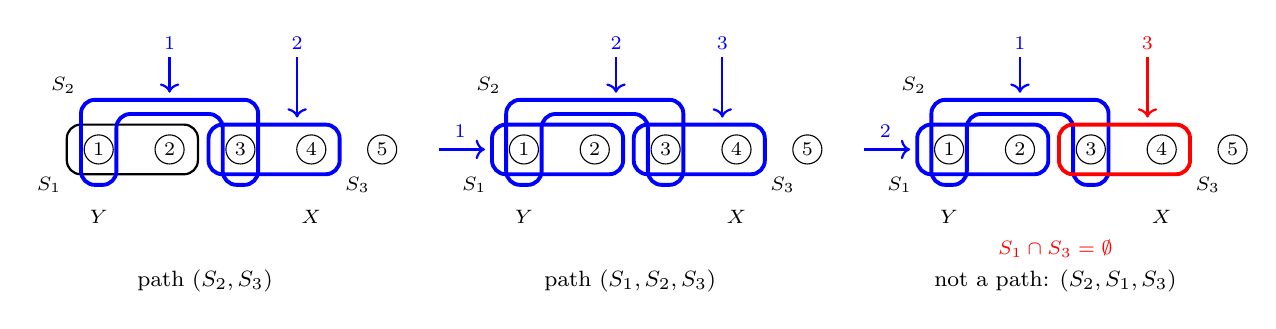
\begin{tikzpicture}[x=0.9cm,y=0.9cm,
  site/.style={circle,draw,fill=white,inner sep=1.6pt,font=\scriptsize},
  edge/.style={rounded corners=5pt,draw,thick,fill=none},
  hl/.style={edge,draw=Blue,line width=1.4pt},
  lab/.style={font=\scriptsize},
  stp/.style={font=\scriptsize,Blue}]
% the arch S2 = {1,3}: legs around sites 1 and 3, joined above site 2
\newcommand{\archtwo}[1]{\draw[#1] (0.75,-0.5) -- (0.75,0.7) -- (3.25,0.7) -- (3.25,-0.5)
    -- (2.75,-0.5) -- (2.75,0.5) -- (1.25,0.5) -- (1.25,-0.5) -- cycle;}
\foreach \dx/\title in {0/{path $(S_2,S_3)$}, 6/{path $(S_1,S_2,S_3)$},
    12/{not a path: $(S_2,S_1,S_3)$}} {
  \begin{scope}[shift={(\dx,0)}]
    \draw[edge] (0.55,-0.35) rectangle (2.4,0.35);               % S1 = {1,2}
    \archtwo{edge}                                              % S2 = {1,3}
    \draw[edge] (2.55,-0.35) rectangle (4.4,0.35);               % S3 = {3,4}
    \foreach \s in {1,...,5} { \node[site] (s\s) at (\s,0) {\s}; }
    \node[lab] at (1,-0.95) {$Y$};
    \node[lab] at (4,-0.95) {$X$};
    \node[lab] at (0.3,-0.5) {$S_1$};
    \node[lab] at (0.5,0.9) {$S_2$};
    \node[lab] at (4.65,-0.5) {$S_3$};
    \node[lab,font=\footnotesize] at (2.5,-1.85) {\title};
  \end{scope}
}
% panel A: S2 then S3
\begin{scope}[shift={(0,0)}]
  \archtwo{hl}
  \draw[hl] (2.55,-0.35) rectangle (4.4,0.35);
  \draw[->,Blue,thick] (2.0,1.3) -- (2.0,0.8); \node[stp] at (2.0,1.5) {$1$};
  \draw[->,Blue,thick] (3.8,1.3) -- (3.8,0.45); \node[stp] at (3.8,1.5) {$2$};
\end{scope}
% panel B: S1, S2, S3 (each crosses the previous one)
\begin{scope}[shift={(6,0)}]
  \draw[hl] (0.55,-0.35) rectangle (2.4,0.35);
  \archtwo{hl}
  \draw[hl] (2.55,-0.35) rectangle (4.4,0.35);
  \draw[->,Blue,thick] (-0.2,0) -- (0.45,0); \node[stp] at (0.1,0.25) {$1$};
  \draw[->,Blue,thick] (2.3,1.3) -- (2.3,0.8); \node[stp] at (2.3,1.5) {$2$};
  \draw[->,Blue,thick] (3.8,1.3) -- (3.8,0.45); \node[stp] at (3.8,1.5) {$3$};
\end{scope}
% panel C: S2, S1, S3 with the gap
\begin{scope}[shift={(12,0)}]
  \archtwo{hl}
  \draw[hl] (0.55,-0.35) rectangle (2.4,0.35);
  \draw[hl,draw=Red] (2.55,-0.35) rectangle (4.4,0.35);
  \draw[->,Blue,thick] (2.0,1.3) -- (2.0,0.8); \node[stp] at (2.0,1.5) {$1$};
  \draw[->,Blue,thick] (-0.2,0) -- (0.45,0); \node[stp] at (0.1,0.25) {$2$};
  \draw[->,Red,thick] (3.8,1.3) -- (3.8,0.45); \node[stp,Red] at (3.8,1.5) {$3$};
  \node[lab,Red] at (2.5,-1.4) {$S_1\cap S_3=\emptyset$};
\end{scope}
\end{tikzpicture}

\caption{\vet{The interaction hypergraph of three terms $S_1=\{1,2\}$, $S_2=\{1,3\}$,
$S_3=\{3,4\}$ on five sites, with $Y=\{1\}$ and $X=\{4\}$. Left: the path $(S_2,S_3)$ of length
two. Middle: the path $(S_1,S_2,S_3)$ of length three; the sequence $(S_2,S_2,S_3)$ is not a
path, because $S_2$ does not cross itself. Right: the sequence $(S_2,S_1,S_3)$ is not a path,
because $S_1$ and $S_3$ do not meet, although each set meets the union of $Y$ and the earlier
ones. Blue marks the sets of the sequence in order, red the step that fails. For unit strengths
the counts are $P_1=0$ and $P_k=1$ for every $k\ge2$, the single path being the alternating
sequence $(S_2,S_1,S_2,\dots,S_3)$ or $(S_1,S_2,S_1,\dots,S_3)$ ending with $S_2,S_3$. With
consecutive overlap in place of crossing, so that a term may follow itself, the first-contact
counts would be $0,1,2,4$; dropping first contact as well gives $0,1,3,8$.}}
\label{fig:hypergraph}
\end{figure}

\begin{proposition}[the path count by recursion]\label{prop:pathcount}
For all regions $X,Y$:
\begin{enumerate}[label=(\alph*),nosep]
\item $P_1(Y,X)=\sum_{i\in I^{\partial Y},\ S_i\cap X\ne\emptyset}\kappa_i$ and, for $k\ge1$,
  $P_{k+1}(Y,X)=\sum_{i\in I^{\partial Y},\ S_i\cap X=\emptyset}\kappa_i\,P_k(S_i,X)$;
\item $0\le P_k(Y,X)\le K^k$ for every $k$ (with $K^0=1$).
\end{enumerate}
\end{proposition}

\begin{proof}
\begin{enumerate}[label=(\alph*),nosep]
\item The paths of length $1$ are the single indices $i$ whose support crosses $Y$ and meets $X$,
of weight $\kappa_i$. A sequence $(i_1,\dots,i_{k+1})$ is a path of length $k+1$ from $Y$ to $X$
exactly when $S_{i_1}$ crosses $Y$ and misses $X$, and $(i_2,\dots,i_{k+1})$ is a path of length
$k$ from $S_{i_1}$ to $X$: the condition ``$S_{i_2}$ crosses $S_{i_1}$'' is the first condition of
the shorter path with $Y$ replaced by $S_{i_1}$, and the remaining conditions are unchanged.
Splitting the sum according to $i_1$ and using $w(i_1,\dots,i_{k+1})=\kappa_{i_1}w(i_2,\dots,i_{k+1})$
gives the recursion.
\item By induction on $k$ using (a): $P_1\le\sum_i\kappa_i=K$ and
$P_{k+1}(Y,X)\le\sum_i\kappa_iK^k=K^{k+1}$.\qedhere
\end{enumerate}
\end{proof}

\begin{example}[two qubits]\label{ex:twosites}
\vet{Two sites $\Lambda=\{0,1\}$, each carrying a qubit, so \vetnew{$\cA=\Mat_2(\C)\otimes\Mat_2(\C)$} with
\vetnew{$\cA(\{0\})=\Mat_2(\C)\otimes1$, $\cA(\{1\})=1\otimes\Mat_2(\C)$}, and the Pauli matrices
$\sigma^x_j,\sigma^y_j,\sigma^z_j$ acting on site $j$. The Hamiltonian is the single term
\[
  H=\sigma^z_0\sigma^z_1,
\]
so the family has one generator, $S_1=\{0,1\}$, $L_1=\ii\comm{H}{\cdot}$ and
$\kappa_1=\norm H=1$ (Example~\ref{ex:hamiltonian}). Take the observable $a=\sigma^x_0$ on
$X=\{0\}$ and the probe $b=\sigma^x_1$ on $Y=\{1\}$. The support $S_1$ crosses $Y$ and meets
$X$, so the only path is $(1)$, of length one: $P_1=1$ and $P_k=0$ for $k\ge2$, since a path of
length two or more would have to miss $X$ at its first step.

The dynamics is explicit. Since $H$ anticommutes with $\sigma^x_0$,
$e^{\ii tH}\sigma^x_0=\sigma^x_0e^{-\ii tH}$, so
$A(t)=\sigma^x_0e^{-2\ii tH}=\sigma^x_0(\cos2t-\ii\sin2t\,\sigma^z_0\sigma^z_1)$ and
\[
  \comm{A(t)}{\sigma^x_1}=-\ii\sin2t\,\sigma^x_0\sigma^z_0\comm{\sigma^z_1}{\sigma^x_1}
  =2\sin2t\,\sigma^x_0\sigma^z_0\sigma^y_1,
\]
of norm $2|\sin2t|$. The path-sum bound of Chapter~\ref{sec:master} will give $4t$.}
\end{example}

\subsection*{Notes and references}
\vet{\vetnew{The net of local algebras is the one of algebraic quantum field theory, restricted to a
lattice. The bound goes back to \cite{lieb-robinson}; its form for interactions on general
lattices, decaying with the distance, is that of \cite{hastings-koma,nachtergaele-sims}.} The
commutator seminorm is the quantity $\sup_{\norm B=1}\norm{\comm AB}$ that the review
\cite{chen-lucas-yin} uses for local approximants (Proposition~4.1 there), here promoted to the
hypothesis (G1). The literature states the dynamics through an interaction $\Phi$
(\cite{nachtergaele-sims}, eqs.~(2.5)--(2.6); \cite{nsy2019}, \S2) or through edge Hamiltonians
$H_e$ (\cite{chen-lucas-yin}, \S3); both are instances of Definition~\ref{def:local-generators}
(Chapters~\ref{sec:qudit} and~\ref{sec:approx}). The crossing condition is that of the chains
of \cite{nsy2019}, eqs.~(3.41)--(3.42), which run over sets meeting the previous set and its
complement (their chains start at the observable's region and ours at the probe's;
Chapter~\ref{sec:master} reconciles the orientation); the sequences of \cite{chen-lucas-yin},
Theorem~3.4, eq.~(3.34), run from a set meeting $Y$ to a set meeting $X$ with consecutive overlap and distinct
consecutive terms, a larger class; the first-contact condition is ours. \emph{Union-chains}, sequences
in which each set meets the union of $Y$ and the earlier sets, are a tempting but wrong
bookkeeping object: the three-term example of Figure~\ref{fig:hypergraph} separates the two
notions, and there are four-term hypergraphs on three sites for which union-chains are not
dominated by the site-matrix bound of Chapter~\ref{sec:closed}, whereas paths always are.}

\paragraph{Checks.} {\small The counts of Figure~\ref{fig:hypergraph} and of
Example~\ref{ex:twosites} are computed by \texttt{checks/m1a\_check.py} and
\texttt{checks/path\_check.py}; the four-term hypergraph is in the latter's section~2.}


\section{The path-sum bound}\label{sec:master}

\motiv{\vet{The commutator $\comm{A(t)}b$ of an evolved observable with a probe $b$ on a region
$Y$ can only be nonzero through the terms of the generator that cross the boundary of $Y$ (a
term inside $Y$ cannot act on an observable supported outside it): with the crossing terms
switched off, the observable's support never grows into $Y$, and causality kills the commutator.
Duhamel's identity isolates exactly the contribution of the switched-off terms, as a time
integral; hypothesis (G1) then replaces the probe $b$ by a probe on the patch $S_i$ of a single
term, one step closer to the observable, and hypothesis (G3) guarantees that the free evolution in
between cannot amplify anything.

Iterating, the commutator is bounded by a sum over paths of
terms leading from $Y$ to $X$, each weighted by the product of its strengths and by the factor $t^k/k!$ that the
nested time integrals produce. \vetnew{This chapter proves that bound,
Theorem~\ref{thm:master}, in five steps: the two analytic lemmas (Duhamel's identity and the
invariance of closed subspaces under the exponential), the support of the restricted dynamics
(a term inside the probe's region annihilates the observables outside it), the one-step
inequality, the iteration with an explicit remainder, and the limit.} Figure~\ref{fig:recursion} shows the mechanism.}}

\needspace{10\baselineskip}
\subsection{Two lemmas on the exponential}\label{subsec:exp}

\begin{lemma}[Duhamel's identity]\label{lem:duhamel}
Let $\mathbb B$ be a complete normed unital real algebra, $R,Q\in\mathbb B$ and $t\in\R$. Then
\begin{equation}\label{eq:duhamel}
  e^{t(R+Q)}=e^{tR}+\int_0^te^{(t-s)R}\,Q\,e^{s(R+Q)}\,ds,
\end{equation}
the integrand being continuous in $s$.
\end{lemma}

\begin{proof}
Let $f(s):=e^{(t-s)R}e^{s(R+Q)}$. For every \vetnew{$G\in\mathbb B$ the map $u\mapsto e^{uG}$ is
differentiable with derivative $Ge^{uG}=e^{uG}G$}, so by the chain rule and the product rule
\[
  f'(s)=-e^{(t-s)R}R\,e^{s(R+Q)}+e^{(t-s)R}(R+Q)\,e^{s(R+Q)}=e^{(t-s)R}\,Q\,e^{s(R+Q)},
\]
a continuous function of $s$. The fundamental theorem of calculus gives
$f(t)-f(0)=\int_0^tf'(s)\,ds$, and $f(t)=e^{t(R+Q)}$, $f(0)=e^{tR}$.
\end{proof}

\begin{lemma}[invariance]\label{lem:invariance}
Let $E$ be a \vetnew{complex Banach space, $M\subseteq E$ a closed complex subspace and $R$ a
bounded complex-linear operator} with $R(M)\subseteq M$. Then $e^{tR}(M)\subseteq M$ for every $t\in\R$.
\end{lemma}

\begin{proof}
For $m\in M$ the partial sums $\sum_{n\le N}t^nR^nm/n!$ lie in $M$, since $R^nm\in M$ by
induction, and they converge in norm to $e^{tR}m$. $M$ is closed.
\end{proof}

\subsection{The restricted dynamics and the first term}\label{subsec:restricted}

\vet{Fix a causal net and a family of local generators. For a region $Y$, write
$L^{\partial Y}:=L_{I^{\partial Y}}$ for the terms crossing $Y$ and
$L':=L_{I\setminus I^{\partial Y}}$ for the rest, the terms disjoint from $Y$ or inside $Y$, so
that $L=L^{\partial Y}+L'$ (Proposition~\ref{prop:subfamilies}).}

\motiv{\vet{\vetnew{The terms inside $Y$ belong with the free part}: an
observable supported outside $Y$ commutes with everything on a
patch inside $Y$, so its commutator seminorm on that patch vanishes, and (G1) then says the term
does nothing to it. Such a term cannot carry a signal out of $Y$. Only the terms that straddle
the boundary of $Y$ can, and they are the perturbation.}}

\begin{proposition}[a term inside the probe's region annihilates the complement]\label{prop:annihilate}
Let the net be causal, $S_i\subseteq Y$ and $c\in\cA(Y^c)$. Then $L_ic=0$.
\end{proposition}

\begin{proof}
Every $b\in\cA(S_i)\subseteq\cA(Y)$ commutes with $c$, since $Y^c$ and $Y$ are disjoint, so
$N_{S_i}(c)=0$ by Proposition~\ref{prop:commnorm}(b), and (G1) gives $\norm{L_ic}\le\kappa_i\cdot0$.
\end{proof}

\begin{proposition}[support of the restricted dynamics]\label{prop:support}
\begin{enumerate}[label=(\alph*),nosep]
\item Let $J\subseteq I$ and let $W$ be a region with $S_i\subseteq W$ for every $i\in J$. Then
  $L_J\,\cA(W)\subseteq\cA(W)$ and $e^{tL_J}\,\cA(W)\subseteq\cA(W)$ for every $t\in\R$.
\item Let the net be causal. Then $L'\,\cA(Y^c)\subseteq\cA(Y^c)$ and
  $e^{tL'}\,\cA(Y^c)\subseteq\cA(Y^c)$ for every $t\in\R$.
\end{enumerate}
\end{proposition}

\begin{proof}
\begin{enumerate}[label=(\alph*),nosep]
\item For $c\in\cA(W)$ and $i\in J$, (G2) gives $L_ic\in\cA(W\cup S_i)=\cA(W)$, and a finite sum of
elements of $\cA(W)$ lies in it. Lemma~\ref{lem:invariance} applies to the closed subspace
$\cA(W)$.
\item A term $i\notin I^{\partial Y}$ either misses $Y$, so that $S_i\subseteq Y^c$ and
(G2) keeps $\cA(Y^c)$ as in (a), or lies inside $Y$, and then $L_ic=0$ for $c\in\cA(Y^c)$ by
Proposition~\ref{prop:annihilate}. Summing, $L'$ maps $\cA(Y^c)$ into itself, and
Lemma~\ref{lem:invariance} applies.\qedhere
\end{enumerate}
\end{proof}

\begin{proposition}[the first term vanishes]\label{prop:first}
Let the net be causal. If $X\cap Y=\emptyset$, $a\in\cA(X)$ and $b\in\cA(Y)$, then
$\comm{e^{tL'}a}{b}=0$ for every $t\in\R$.
\end{proposition}

\begin{proof}
$X\subseteq Y^c$, so $a\in\cA(Y^c)$ and $e^{tL'}a\in\cA(Y^c)$ by
Proposition~\ref{prop:support}(b); $Y^c$ and $Y$ are disjoint, so causality gives the claim.
\end{proof}

\subsection{The one-step inequality}\label{subsec:onestep}

\needspace{10\baselineskip}
\begin{proposition}[the reset step]\label{prop:reset}
For $s\le t$, $c\in\cA$ and $b\in\cA$ with $\norm b\le1$,
\[
  \bigl\lVert\comm{e^{(t-s)L'}\,L^{\partial Y}c}{b}\bigr\rVert\le2\sum_{i\in I^{\partial Y}}\kappa_i\,N_{S_i}(c).
\]
\end{proposition}

\begin{proof}
$\norm{\comm{c'}b}\le2\norm{c'}$ for every $c'\in\cA$ and $\norm b\le1$; $\norm{e^{(t-s)L'}}\le1$
by (G3) for the sub-family $I\setminus I^{\partial Y}$ and $t-s\ge0$; and
$\norm{L^{\partial Y}c}\le\sum_{i\in I^{\partial Y}}\kappa_iN_{S_i}(c)$ by
Proposition~\ref{prop:subfamilies}(c).
\end{proof}

\begin{figure}[t]
\centering
% Figure 2: the probe-reset recursion. Transcription (for cheap agents): a tree. Root node
% "C_{X,Y}(t)" (commutator of A(t) on X with a probe on Y). One Duhamel step splits it into
% "2[X meets Y]" (the trivial bound when the regions meet; for disjoint regions the free term of
% the Duhamel step is zero) plus, for each term i crossing Y (meeting Y and its complement), a
% branch labelled "2 kappa_i int_0^t ... ds" leading to the node "C_{X,S_i}(s)" (the same
% commutator with a probe on S_i). Branches whose S_i meets X stop with the trivial bound "<= 2";
% the others split again in the same way. The sequence of patches along a root-to-leaf branch is
% a first-contact path. Each branch label is written horizontally near the lower end of its
% arrow, on the outer side (left of a left branch, right of a right branch), clear of the other
% arrows; the free-term node sits higher, to the far left, with its note below it. The dashed
% arrow to the further branches leaves the root to the right and turns down to the dots.
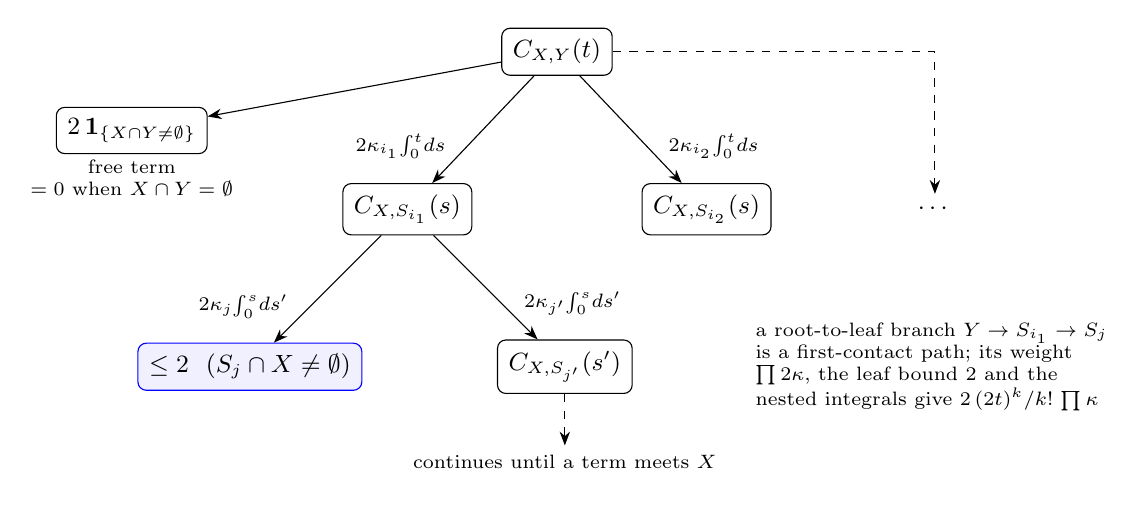
\begin{tikzpicture}[x=1cm,y=1cm,
  node/.style={draw,rounded corners=3pt,inner sep=4pt,font=\small,fill=white},
  leaf/.style={node,draw=Blue,fill=Blue!6},
  lab/.style={font=\scriptsize,fill=white,inner sep=1pt},
  >={Stealth[length=5pt]}]
\node[node] (root) at (0,0) {$C_{X,Y}(t)$};
\node[node] (free) at (-5.4,-1.0) {$2\,\ind{X\cap Y\ne\emptyset}$};
\node[lab,below=1pt of free,align=center] {free term\\ $=0$ when $X\cap Y=\emptyset$};
\node[node] (i1) at (-1.9,-2.0) {$C_{X,S_{i_1}}(s)$};
\node[node] (i2) at (1.9,-2.0) {$C_{X,S_{i_2}}(s)$};
\node[font=\small] (dots) at (4.8,-2.0) {$\cdots$};
\draw[->] (root) -- (free);
\draw[->] (root) -- (i1) node[lab,pos=0.82,above left=1pt]{$2\kappa_{i_1}\!\int_0^t\!ds$};
\draw[->] (root) -- (i2) node[lab,pos=0.82,above right=1pt]{$2\kappa_{i_2}\!\int_0^t\!ds$};
\draw[->,dashed] (root.east) -| (dots.north);
% second level under i1: one branch stops (meets X), one continues
\node[leaf] (stop) at (-3.9,-4.0) {$\le2$ \ ($S_{j}\cap X\ne\emptyset$)};
\node[node] (cont) at (0.1,-4.0) {$C_{X,S_{j'}}(s')$};
\draw[->] (i1) -- (stop) node[lab,pos=0.82,above left=1pt]{$2\kappa_{j}\!\int_0^s\!ds'$};
\draw[->] (i1) -- (cont) node[lab,pos=0.82,above right=1pt]{$2\kappa_{j'}\!\int_0^s\!ds'$};
\draw[->,dashed] (cont) -- ++(0,-1.0) node[below,font=\scriptsize]{continues until a term meets $X$};
\node[font=\scriptsize,align=left,anchor=west] at (2.4,-4.0)
  {a root-to-leaf branch $Y\to S_{i_1}\to S_j$\\ is a first-contact path; its weight\\
   $\prod 2\kappa$, the leaf bound $2$ and the\\ nested integrals give $2\,(2t)^k/k!\,\prod\kappa$};
\end{tikzpicture}

\caption{\vet{The probe-reset recursion. The commutator of the evolved observable $A(t)$ on $X$
with a probe on $Y$ is bounded, after one Duhamel step, by the terms $S_i$ crossing $Y$, each
contributing $2\kappa_i$ times a time integral of the same commutator with a probe on $S_i$. The
recursion stops at the first term meeting $X$, where the trivial bound $2$ is used; the chain of
patches visited is a path of Definition~\ref{def:path}.}}
\label{fig:recursion}
\end{figure}

\vet{The reset step is where the probe moves: on the right-hand side the commutator with the
original probe $b$ has become the seminorm $N_{S_i}(c)$, a supremum of commutators with probes
on the single patch $S_i$. The next statement packages one application of Duhamel's identity
with this step. It takes an arbitrary continuous majorant of the reset seminorms, because that
is how the induction will consume it. The theorem needs the regions disjoint, so a probe on a
patch that meets $X$ cannot be reset again; there the trivial bound $2$ of
Proposition~\ref{prop:commnorm}(a) is used instead. This is why paths end at first contact.}

\begin{theorem}[one Duhamel step]\label{thm:onestep}
Let the net be causal, $X\cap Y=\emptyset$, $a\in\cA(X)$, $b\in\cA(Y)$ with $\norm b\le1$,
$t\ge0$, and let $\beta_i:\R\to\R$ ($i\in I^{\partial Y}$) be continuous functions with
$N_{S_i}(A(s))\le\beta_i(s)$ for all $s\in[0,t]$. Then
\begin{equation}\label{eq:onestep}
  \norm{\comm{A(t)}b}\le2\sum_{i\in I^{\partial Y}}\kappa_i\int_0^t\beta_i(s)\,ds .
\end{equation}
\end{theorem}

\begin{proof}
Lemma~\ref{lem:duhamel} with $R=L'$ and $Q=L^{\partial Y}$, applied to $a$, gives
$A(t)=e^{tL'}a+\int_0^te^{(t-s)L'}L^{\partial Y}A(s)\,ds$. Evaluation at $a$ and the commutator
with $b$ are bounded linear maps and pass through the integral:
\[
  \comm{A(t)}b=\comm{e^{tL'}a}{b}+\int_0^t\comm{e^{(t-s)L'}L^{\partial Y}A(s)}{b}\,ds .
\]

The first term is $0$ by Proposition~\ref{prop:first}. The norm of the integral is at most the
integral of the norm, which Proposition~\ref{prop:reset} with $c=A(s)$ bounds pointwise by
$2\sum_{i\in I^{\partial Y}}\kappa_iN_{S_i}(A(s))\le2\sum_{i\in I^{\partial Y}}\kappa_i\beta_i(s)$,
a continuous function.
\end{proof}

\subsection{The iteration and the series}\label{subsec:iteration}

\vet{For $k\ge0$ and $t\in\R$ put $\gamma_k(t):=(2t)^{k+1}/(k+1)!$, and for regions $X,Y$,
$n\ge0$ and $t\in\R$ (a polynomial in $t$, used for $t\ge0$),
\begin{equation}\label{eq:truncbound}
  B_n(Y,X,t):=2\Bigl(\sum_{k<n}\gamma_k(t)\,P_{k+1}(Y,X)+\gamma_n(t)\,K^{n+1}\Bigr),
\end{equation}
the truncated series with its remainder. The identity $\int_0^t\gamma_k(s)\,ds=\gamma_{k+1}(t)/2$
is what makes the time-ordered integrals produce the factorials.}

\begin{theorem}[iteration]\label{thm:iteration}
Let the net be causal, $X\cap Y=\emptyset$, $a\in\cA(X)$, $b\in\cA(Y)$ with
$\norm a,\norm b\le1$, and $t\ge0$.
Then $\norm{\comm{A(t)}b}\le B_n(Y,X,t)$ for every $n\ge0$.
\end{theorem}

\begin{proof}
Induction on $n$, for all disjoint pairs $X,Y$, all $t\ge0$ and all $a,b$ of norm at most $1$
at once.

\emph{Base.} Theorem~\ref{thm:onestep} with the constant majorants $\beta_i=2$, legitimate since
$N_{S_i}(A(s))\le2\norm{A(s)}\le2$ by Propositions~\ref{prop:commnorm}(a)
and~\ref{prop:subfamilies}(b), gives $\norm{\comm{A(t)}b}\le4t\sum_{i\in I^{\partial Y}}\kappa_i\le4tK
=B_0(Y,X,t)$.

\emph{Step.} Assume the bound for $n$. Apply Theorem~\ref{thm:onestep} with the majorant
$\beta_i(s)=2$ when $S_i$ meets $X$, and $\beta_i(s)=B_n(S_i,X,s)$ when $S_i$ misses $X$; the
latter is
a majorant because, for every unit $b'\in\cA(S_i)$, the induction hypothesis for the disjoint
pair $(X,S_i)$ gives $\norm{\comm{A(s)}{b'}}\le B_n(S_i,X,s)$, and $N_{S_i}(A(s))$ is the
supremum of these. Integrating \eqref{eq:truncbound} with the identity for $\int\gamma_k$,
\[
  \int_0^tB_n(S_i,X,s)\,ds=\sum_{k<n}\gamma_{k+1}(t)\,P_{k+1}(S_i,X)+\gamma_{n+1}(t)\,K^{n+1}.
\]

Summing over $i\in I^{\partial Y}$ with the weights $2\kappa_i$: the terms meeting $X$ contribute
$2\gamma_0(t)\sum\kappa_i=2\gamma_0(t)P_1(Y,X)$; the terms missing $X$ contribute
$2\sum_{k<n}\gamma_{k+1}(t)\sum_i\kappa_iP_{k+1}(S_i,X)=2\sum_{k<n}\gamma_{k+1}(t)P_{k+2}(Y,X)$ by
the recursion of Proposition~\ref{prop:pathcount}(a), and a remainder
$2\gamma_{n+1}(t)K^{n+1}\sum_i\kappa_i\le2\gamma_{n+1}(t)K^{n+2}$, where the sum over the terms
missing $X$ is at most $K$. Together this is $B_{n+1}(Y,X,t)$: the first group is the $k=0$
term of the sum in \eqref{eq:truncbound} for $n+1$, the second group its terms $k=1,\dots,n$,
and the remainder its last term.
\end{proof}

\begin{theorem}[the path-sum bound]\label{thm:master}
Let the net be causal and $t\ge0$. For regions $X,Y$, $a\in\cA(X)$ and $b\in\cA(Y)$,
\begin{equation}\label{eq:master}
  \norm{\comm{A(t)}b}\le2\norm a\norm b\Bigl(\ind{X\cap Y\ne\emptyset}
  +\sum_{k\ge1}\frac{(2t)^k}{k!}\,P_k(Y,X)\Bigr),
\end{equation}
where $\ind{P}$ is the indicator of a condition $P$, $1$ if it holds and $0$ otherwise; the series converges, with
sum at most $e^{2tK}-1$. Equivalently, for
$C_{X,Y}(t):=\sup\{\norm{\comm{e^{tL}a}b}:a\in\cA(X),b\in\cA(Y),\norm a,\norm b\le1\}$,
\[
  C_{X,Y}(t)\le2\,\ind{X\cap Y\ne\emptyset}+2\sum_{k\ge1}\frac{(2t)^k}{k!}\,P_k(Y,X).
\]
\end{theorem}

\begin{proof}
The $k$-th term is at most $(2tK)^k/k!$ by Proposition~\ref{prop:pathcount}(b), so the series
converges. If $X$ meets $Y$ the bound $2\norm a\norm b$ holds since $\norm{A(t)}\le\norm a$. If
$X\cap Y=\emptyset$ and $a,b$ are unit, Theorem~\ref{thm:iteration} gives, for every $n$, the
truncated series plus $2(2tK)^{n+1}/(n+1)!$, which tends to $0$; the truncated series is at most
the full one. General $a,b$ follow by scaling, and the supremum form by taking the supremum.
\end{proof}

\begin{example}[two qubits, continued]\label{ex:twosites-bound}
\vet{For $H=\sigma^z_0\sigma^z_1$, $a=\sigma^x_0$ and $b=\sigma^x_1$ (Example~\ref{ex:twosites}),
$P_1=1$ and $P_k=0$ for $k\ge2$, so Theorem~\ref{thm:master} gives
$\norm{\comm{A(t)}b}\le2\cdot2t=4t$. The exact value $2|\sin2t|$ lies below $4t$ and matches
it to first order: the constant $2\kappa$ per step is not loose at short times.}
\end{example}

\begin{example}[a three-qubit chain]\label{ex:chain}
\vet{Three qubits on $\Lambda=\{0,1,2\}$ with the Hamiltonian
\[
  H=\sigma^z_0\sigma^z_1+\tfrac12\,\sigma^x_1\sigma^x_2 ,
\]
that is, two terms: $\Phi_1=\sigma^z_0\sigma^z_1$ on $S_1=\{0,1\}$ with $\kappa_1=1$, and
$\Phi_2=\tfrac12\sigma^x_1\sigma^x_2$ on $S_2=\{1,2\}$ with $\kappa_2=\tfrac12$. The observable
is $a=\sigma^x_0$ on $X=\{0\}$, the probe $b=\sigma^z_2$ on $Y=\{2\}$.

\emph{The paths.} Only $S_2$ crosses $Y$, and it misses $X$; after it only $S_1$ can follow,
since $S_1$ crosses $S_2$ while $S_2$ does not cross itself, and $S_1$ meets $X$. So the only
path is $(S_2,S_1)$: $P_2=\kappa_1\kappa_2=\tfrac12$, every other $P_k$ is $0$, and
Theorem~\ref{thm:master} gives
\[
  \norm{\comm{A(t)}{\sigma^z_2}}\le2\cdot\frac{(2t)^2}{2!}\cdot\frac12=2t^2\qquad\vetnew{\text{for every }t\ge0}.
\]

\vetnew{\emph{The exact value.} The three Pauli strings $\mathbf e_0=\sigma^x_0$,
$\mathbf e_1=\sigma^y_0\sigma^z_1$, $\mathbf e_2=\sigma^y_0\sigma^y_1\sigma^x_2$ satisfy
$\comm H{\mathbf e_0}=2\ii\mathbf e_1$, $\comm H{\mathbf e_1}=-2\ii\mathbf e_0-\ii\mathbf e_2$,
$\comm H{\mathbf e_2}=\ii\mathbf e_1$, so
$A(t)=f_0(t)\mathbf e_0+f_1(t)\mathbf e_1+f_2(t)\mathbf e_2$ with $f_0'=2f_1$,
$f_1'=-2f_0-f_2$, $f_2'=f_1$ and $(f_0,f_1,f_2)(0)=(1,0,0)$; hence
$f_2(t)=\tfrac25(\cos\sqrt5\,t-1)$. Only $\mathbf e_2$ fails to commute with the probe,
$\comm{\mathbf e_2}{\sigma^z_2}=-2\ii\,\sigma^y_0\sigma^y_1\sigma^y_2$, so}
\[
  \norm{\comm{A(t)}{\sigma^z_2}}=\vetnew{2|f_2(t)|}=\tfrac45\bigl(1-\cos\sqrt5\,t\bigr)
  =2t^2-\tfrac56t^4+O(t^6).
\]
The ratio to the bound is $1-\tfrac5{12}t^2+\dots$, equal to $0.99996$ at $t=0.01$ and
decreasing; the bound is never exceeded. On this chain the path-sum bound is sharp to leading
order at short times, while at long times every commutator is at most $2$ and the bound grows.}
\end{example}

\subsection*{Route against the source}
\vet{The sources differentiate the commutator in time and move the derivative onto the probe
with the Jacobi identity. Writing $f(t)=\comm{\tau_t(A)}B$ and
$\frac{d}{dt}\tau_t(A)=\ii\comm{\tau_t(H_X)}{\tau_t(A)}$ with $H_X$ the terms meeting the
observable's region, \cite{nsy2019} (eqs.~(3.40)--(3.48)) and \cite{nachtergaele-sims} obtain
$f'=\ii\comm{\tau_t(H_X)}{f}-\ii\comm{\tau_t(A)}{\comm{\tau_t(H_X)}B}$; the first term generates a
norm-preserving flow and drops out of the norm estimate, the second resets the observable to a
single term $\Phi(Z)$ with $Z\cap X\ne\emptyset$, and iterating gives a series over chains of
overlapping supports. The review \cite{chen-lucas-yin} (eqs.~(3.26)--(3.29)) does the same in
graph language.

The route above differs in three respects. It integrates (Duhamel) instead of
differentiating, so that no Jacobi identity and no derivation property are needed, and the
hypotheses reduce to (G1)--(G3); the open-system bound of Chapter~\ref{sec:approx} is therefore
the same theorem. It resets the probe rather than the observable, which is a matter of taste.
And it stops at first contact, which the sources do not. The path class is otherwise theirs.

The chains of \cite{nsy2019}, eqs.~(3.41)--(3.42), are sequences $Z_1,\dots,Z_n$ with $Z_1$
meeting the observable's region and its complement, each $Z_{j+1}$ meeting $Z_j$ and its
complement, and $Z_n$ meeting the probe's region; they run from the observable to the probe
because the source resets the observable. For an automorphism group
$\norm{\comm{\tau_t(A)}B}=\norm{\comm{A}{\tau_{-t}(B)}}$ and the source's bound depends on $|t|$,
so its theorem applied to the pair $(B,A)$ runs the chains from $Y$: $Z_1$ crosses $Y$ and each
$Z_{j+1}$ crosses $Z_j$, which is Definition~\ref{def:path} without first contact. With one
term per support and $\kappa_Z=\norm{\Phi(Z)}$, the weights $2\norm{\Phi(Z_j)}$ and the
nested integrals $t^n/n!$ are the same, so in the Hamiltonian case the series \eqref{eq:master}
is at most the chain series of \cite{nsy2019} term by term.

The reason the sources may restrict
to crossing sets is the one of Proposition~\ref{prop:annihilate}: a term inside the current
region cannot move an observable supported outside it. The review's recursion (3.29b) drops the
repeated edge without giving this reason; Proposition~\ref{prop:annihilate} supplies it.

The review's Theorem~3.4 sums over sequences from a set meeting $Y$ to a set meeting $X$ with
consecutive overlap and distinct consecutive terms, a class containing ours since a set crossing
another differs from it, so \eqref{eq:master} is at most that series as well; the review
attributes the theorem to the work it numbers [34], and the stronger irreducible-path bound of
\cite{chen-lucas2021}, Theorem~3, is not claimed here.}

\subsection*{Notes and references}
\vet{Theorem~\ref{thm:master} is the generator-level form of the Lieb-Robinson path series,
Theorem~3.4 of \cite{chen-lucas-yin} and eqs.~(3.41)--(3.42) of \cite{nsy2019}, with the
differences listed above; its constants, $2\kappa_i$ per step and $t^k/k!$, are theirs.
Duhamel's identity and the invariance lemma are standard; both are proved here for a general
complete normed unital real algebra and a general Banach space.}

\paragraph{Checks.} {\small The numbers of Example~\ref{ex:chain} are computed by
\texttt{checks/m1a\_crossing\_check.py} and \texttt{checks/m1a\_chain\_expansion\_check.py},
the latter also for the closed form of the commutator norm.}


\FloatBarrier
\section{Closed forms and light cones}\label{sec:closed}

\motiv{\vet{The path-sum bound of Chapter~\ref{sec:master} is exact bookkeeping: it counts the
sequences of terms that can carry a signal. To read it as a statement about distances, we
replace the count of paths by something that only sees pairs of sites, the \emph{site matrix},
whose entry at $(u,u')$ adds up the strengths of the terms containing both sites. A path of $k$
terms visits $k+1$ sites, one in the probe's region, one in each of the $k-1$ overlaps of
consecutive supports, and one in the observable's region; its weight is at most the product of
the matrix entries along those sites. Summing over all site sequences gives an entry of the
$k$-th power of the matrix, and summing the series gives its exponential.

From there the
published forms follow by three estimates: a decay function bounds the entries, a bounded
geometry bounds the row sums and makes distant entries of the powers vanish, and the tail of the
exponential series gives the light cone. \vetnew{A last section extends all of these to negative
times when the negated generators are contractive as well, as they are for a Hamiltonian.}}}

\subsection{The site matrix and walks}\label{subsec:sitematrix}

\vet{Throughout, $(S_i,L_i,\kappa_i)_{i\in I}$ is a family of local generators on a causal net
over an arbitrary set of sites $\Lambda$, and $T:=\bigcup_iS_i$ is the finite set of
\revs{\emph{touched sites}, the sites the family touches}. We write $\chi_i(u):=\ind{u\in S_i}$ for the indicator of a support.}

\begin{definition}[site matrix, walks]\label{def:sitematrix}
\vet{The \emph{site matrix} of the family is
\begin{equation}\label{eq:h}
  h_{uu'}:=\sum_{i\in I:\ u\in S_i,\ u'\in S_i}\kappa_i=\sum_i\kappa_i\,\chi_i(u)\,\chi_i(u')
  \qquad(u,u'\in\Lambda),
\end{equation}
so that $h_{uu}=\sum_{i\ni u}\kappa_i$. The \emph{walk weights} are defined by
$w_0(y,x):=\ind{y=x}$ and
\begin{equation}\label{eq:walk}
  w_{k+1}(y,x):=\sum_{z\in T}h_{yz}\,w_k(z,x).
\end{equation}
For a region $Y$, the \emph{boundary} $\bd Y:=Y\cap\bigcup_{i\in I^{\bd Y}}S_i$ is the set of
sites of $Y$ touched by a term crossing $Y$. For regions $Y,X$ put
\begin{equation}\label{eq:W}
  W_k(Y,X):=\sum_{y\in\bd Y}\ \sum_{x\in X\cap T}w_k(y,x).
\end{equation}}
\end{definition}

\vet{$w_k(y,x)$ is the total weight of the walks of $k$ steps from $y$ to $x$ through the
touched sites, each step $z\to z'$ weighted by $h_{zz'}$; on a finite lattice it is the entry
$(h^k)_{yx}$ (Proposition~\ref{prop:finite}). A walk may stay at a site, weighted by the diagonal
of $h$, or return to one. The boundary $\bd Y$ is the part of the probe's region that the
dynamics can reach from outside: a term inside $Y$ does nothing to an observable supported
outside $Y$ (Proposition~\ref{prop:annihilate}), so a signal enters $Y$ only through the sites
that a crossing term touches. Both $\bd Y$ and $X\cap T$ are finite, so $W_k$ is a finite sum.}

\needspace{10\baselineskip}
\begin{proposition}[properties]\label{prop:walkprops}
\vet{Let $K_1:=\sum_i\kappa_i|S_i|$.
\begin{enumerate}[label=(\alph*),nosep]
\item $h_{uu'}\ge0$, $h_{uu'}=h_{u'u}$, and $h_{uu'}=0$ unless $u,u'\in T$;
\item \vetnew{$\sum_{u'\in T}h_{uu'}\le K_1$ for every site $u$};
\item $w_k(y,x)\ge0$; for $k\ge1$, $w_k(y,x)=0$ unless $y,x\in T$, and $w_1(y,x)=h_{yx}$;
\item $\sum_{x\in T}w_k(y,x)\le q^k$ whenever every row sum $\sum_{u'\in T}h_{uu'}$ is at most
  $q\ge0$; hence $W_k(Y,X)\le|\bd Y|\,q^k$, and in particular $W_k(Y,X)\le|\bd Y|\,K_1^{\,k}$.
\end{enumerate}}
\end{proposition}

\begin{proof}
\vet{\begin{enumerate}[label=(\alph*),nosep]
\item Read off the definitions.
\item Exchanging the sums, $\sum_{u'\in T}\sum_{i:\,u,u'\in S_i}\kappa_i=\sum_{i\ni u}\kappa_i|S_i|\vetnew{{}\le K_1}$.
\item Read off the definitions.
\item By induction on $k$: for $k=0$ the sum is $\ind{y\in T}\le1$, and
$\sum_xw_{k+1}(y,x)=\sum_zh_{yz}\sum_xw_k(z,x)\le q^k\sum_zh_{yz}\le q^{k+1}$.\qedhere
\end{enumerate}}
\end{proof}

\vetnew{The proof of (b) gives the row sum exactly: $\sum_{u'\in T}h_{uu'}=\sum_{i\ni u}\kappa_i|S_i|$,
the total weighted size of the supports that contain $u$.}

\begin{figure}[t]
\centering
% Figure: a path of three terms from Y to X and a sequence of sites along it. Transcription (for
% cheap agents): seven sites 0..6 on a line; the probe's region Y = {0, 1} (left box), the
% observable's region X = {5, 6} (right box); three supports drawn as rounded boxes above the
% line: S_{i_1} = {1, 2, 3}, S_{i_2} = {3, 4}, S_{i_3} = {4, 5}; the chosen sites u_0 = 1 (in
% S_{i_1} ∩ Y, on the boundary of Y), u_1 = 3 (in S_{i_1} ∩ S_{i_2}), u_2 = 4 (in S_{i_2} ∩ S_{i_3}),
% u_3 = 5 (in S_{i_3} ∩ X), marked by filled circles and joined by arrows labelled h_{13}, h_{34},
% h_{45}; the weights κ_{i_1} ≤ h_{13}, κ_{i_2} ≤ h_{34}, κ_{i_3} ≤ h_{45} written under the arrows.
% The label S_{i_3} sits above the box S_{i_3}, clear of the box S_{i_2}; the label u_3 sits
% slightly to the right of site 5, above the box of X, clear of S_{i_3}.
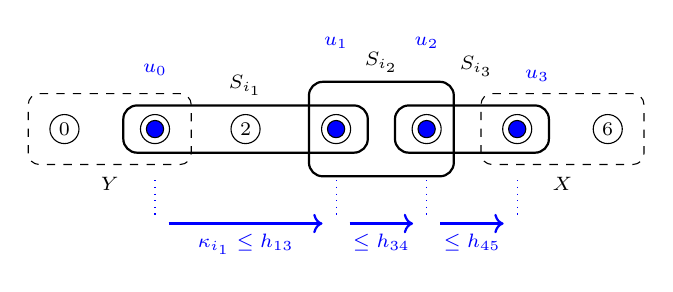
\begin{tikzpicture}[x=1.15cm,y=1cm,
  site/.style={circle,draw,fill=white,inner sep=1.6pt,font=\scriptsize},
  chosen/.style={circle,draw,fill=Blue,inner sep=2.2pt},
  edge/.style={rounded corners=5pt,draw,thick,fill=none},
  region/.style={rounded corners=4pt,draw,dashed,fill=none},
  lab/.style={font=\scriptsize}]
  % regions
  \draw[region] (-0.4,-0.45) rectangle (1.4,0.45);
  \node[lab] at (0.5,-0.7) {$Y$};
  \draw[region] (4.6,-0.45) rectangle (6.4,0.45);
  \node[lab] at (5.5,-0.7) {$X$};
  % supports
  \draw[edge] (0.65,-0.3) rectangle (3.35,0.3);   \node[lab] at (2,0.55) {$S_{i_1}$};
  \draw[edge] (2.7,-0.6) rectangle (4.3,0.6);     \node[lab] at (3.5,0.85) {$S_{i_2}$};
  \draw[edge] (3.65,-0.3) rectangle (5.35,0.3);   \node[lab] at (4.55,0.8) {$S_{i_3}$};
  % sites
  \foreach \s in {0,...,6} { \node[site] (s\s) at (\s,0) {\s}; }
  \node[chosen] at (1,0) {}; \node[chosen] at (3,0) {}; \node[chosen] at (4,0) {};
  \node[chosen] at (5,0) {};
  \node[lab,Blue] at (1,0.75) {$u_0$};
  \node[lab,Blue] at (3,1.1) {$u_1$};
  \node[lab,Blue] at (4,1.1) {$u_2$};
  \node[lab,Blue] at (5.22,0.68) {$u_3$};
  % the walk
  \draw[->,Blue,thick] (1.15,-1.2) -- (2.85,-1.2) node[midway,below,lab,Blue] {$\kappa_{i_1}\le h_{13}$};
  \draw[->,Blue,thick] (3.15,-1.2) -- (3.85,-1.2) node[midway,below,lab,Blue] {$\le h_{34}$};
  \draw[->,Blue,thick] (4.15,-1.2) -- (4.85,-1.2) node[midway,below,lab,Blue] {$\le h_{45}$};
  \foreach \s in {1,3,4,5} { \draw[Blue,dotted,thin] (\s,-0.65) -- (\s,-1.1); }
\end{tikzpicture}

\caption{\vet{A path of three terms from the probe's region $Y$ to the observable's region $X$,
and a sequence of sites along it: $u_0\in S_{i_1}\cap Y$ lies on the boundary $\bd Y$, each
$u_j$ in the overlap $S_{i_j}\cap S_{i_{j+1}}$, and $u_3\in S_{i_3}\cap X$. Each step
$u_{j-1}\to u_j$ stays inside the support $S_{i_j}$, so $\kappa_{i_j}\le h_{u_{j-1}u_j}$: the
weight of the path is at most the weight of this walk. Theorem~\ref{thm:domination} makes the
idea precise without choosing the sites, by expanding the walk sum through the indicators of
the supports.}}
\label{fig:walkchoice}
\end{figure}

\begin{theorem}[domination of the path count]\label{thm:domination}
\vet{For every $k\ge1$ and all regions $X,Y$,
\begin{equation}\label{eq:domination}
  P_k(Y,X)\le W_k(Y,X).
\end{equation}}
\end{theorem}

\begin{proof}
\vet{Induction on $k$, the claim quantified over all $Y$.

\emph{$k=1$.} $P_1(Y,X)$ is the sum of $\kappa_i$ over the terms crossing $Y$ and meeting $X$.
Expanding \eqref{eq:W} with $w_1=h$ and \eqref{eq:h},
\[
  W_1(Y,X)=\sum_i\kappa_i\Bigl(\sum_{y\in\bd Y}\chi_i(y)\Bigr)\Bigl(\sum_{x\in X\cap T}\chi_i(x)\Bigr).
\]
For a term $i$ crossing $Y$ and meeting $X$, some site of $S_i$ lies in $Y$, hence in $\bd Y$,
and some site of $S_i$ lies in $X$, hence in $X\cap T$; so both brackets are at least $1$.
Every other term contributes a nonnegative amount. Hence $P_1\le W_1$.

\emph{Step, the left side.} The recursion of Proposition~\ref{prop:pathcount} gives
$P_{k+1}(Y,X)=\sum_{i\in Q}\kappa_iP_k(S_i,X)$, with $Q$ the terms crossing $Y$ and missing $X$.
\vetnew{We extend the notation: $w_k(z,X):=\sum_{x\in X\cap T}w_k(z,x)\ge0$. By the induction
hypothesis for the region $S_i$, and since $\bd S_i\subseteq S_i$,
$P_k(S_i,X)\le W_k(S_i,X)\le\sum_{z\in S_i}w_k(z,X)$.}

\emph{Step, the right side.} Expanding \eqref{eq:W} with \eqref{eq:walk} and \eqref{eq:h}, and
summing over $z$ first,
\[
  W_{k+1}(Y,X)=\sum_i\kappa_i\Bigl(\sum_{y\in\bd Y}\chi_i(y)\Bigr)\sum_{z\in S_i}\vetnew{w_k(z,X)}.
\]

\emph{Comparison.} For $i\in Q$ the bracket is at least $1$, as in the base case, and every
other term is nonnegative. So
$P_{k+1}(Y,X)\le\sum_{i\in Q}\kappa_i\sum_{z\in S_i}\vetnew{w_k(z,X)}\le W_{k+1}(Y,X)$.}
\end{proof}

\vet{What the domination loses: a walk may return to a site it has visited, while a path never
repeats a term immediately, and a walk continues after reaching $X$, while a path stops. Both
effects are visible in Example~\ref{ex:chainwalk}, where equality holds at $k=2$ and the walk
weights are strictly larger from $k=3$ on.}

\subsection{The walk series and the matrix exponential}

\begin{theorem}[closed form (i): the walk series]\label{thm:walkseries}
\vet{Let the net be causal, $t\ge0$, $a\in\cA(X)$ and $b\in\cA(Y)$. Then
\begin{equation}\label{eq:walkseries}
  \norm{\comm{A(t)}b}\le2\norm a\norm b\Bigl(\ind{X\cap Y\ne\emptyset}
  +\sum_{k\ge1}\frac{(2t)^k}{k!}\,W_k(Y,X)\Bigr),
\end{equation}
the series converging with sum at most $|\bd Y|\,(e^{2K_1t}-1)$.}
\end{theorem}

\begin{proof}
\vet{Termwise, $(2t)^kP_k/k!\le(2t)^kW_k/k!\le|\bd Y|(2tK_1)^k/k!$ by Theorem~\ref{thm:domination}
and Proposition~\ref{prop:walkprops}(d); so the walk series converges by comparison with the
exponential series, and \eqref{eq:master} gives \eqref{eq:walkseries}.}
\end{proof}

\vetnew{The terms of this series are the \emph{walk terms}: for the pair $(Y,X)$ and $k\ge0$,
\begin{equation}\label{eq:walkterms}
  \omega_k(t):=\frac{(2t)^{k+1}}{(k+1)!}\,W_{k+1}(Y,X)=\gamma_k(t)\,W_{k+1}(Y,X),
\end{equation}
with the coefficient $\gamma_k$ of \eqref{eq:truncbound}, so that the series in
\eqref{eq:walkseries} is $\sum_{k\ge0}\omega_k(t)$. We shift the index by one so that
$\omega_k$ carries the walks of $k+1$ steps as $\gamma_k$ carries the paths of length $k+1$. The
walk terms depend on the strengths $\kappa_i$, through the site matrix in $W_{k+1}$, and on the
pair $(Y,X)$; Chapter~\ref{sec:approx} uses them.}

\begin{proposition}[finite lattice]\label{prop:finite}
\vet{Let $\Lambda$ be finite and regard $h$ as a matrix. Then $w_k(y,x)=(h^k)_{yx}$, and for
$s\in\R$ the entries of the matrix exponential are the series of the entries of the powers,
$(e^{sh})_{yx}=\sum_{n\ge0}s^n(h^n)_{yx}/n!$. Consequently
\begin{equation}\label{eq:matrixform}
  \norm{\comm{A(t)}b}\le2\norm a\norm b\Bigl(\ind{X\cap Y\ne\emptyset}
  +\sum_{y\in\bd Y}\sum_{x\in X\vetnew{{}\cap T}}\bigl(e^{2th}-1\bigr)_{yx}\Bigr).
\end{equation}}
\end{proposition}

\begin{proof}
\vet{$w_{k+1}(y,x)=\sum_{z\in T}h_{yz}(h^k)_{zx}=\sum_{z\in\Lambda}h_{yz}(h^k)_{zx}$, the terms
with $z\notin T$ vanishing, which is $(h^{k+1})_{yx}$. The exponential series converges in any
algebra norm on the matrices, and every entry is bounded by the norm, so the entries converge to
the entries. Then \eqref{eq:matrixform} is \eqref{eq:walkseries} with the series summed
entrywise\vetnew{, over the pairs of $\bd Y\times(X\cap T)$ as in \eqref{eq:W}}.}
\end{proof}

\vetnew{The inner sum in \eqref{eq:matrixform} may equally run over all of $X$: for $x\notin T$
the column $x$ of $h$ vanishes, so $(h^n)_{yx}=0$ for $n\ge1$ and the entry
$(e^{2th}-1)_{yx}$ is zero.}

\vet{Inequality \eqref{eq:matrixform} is the matrix form of the Lieb-Robinson bound in
\cite{chen-lucas-yin}, with the sum over the probe's region sharpened to its boundary.}

\begin{example}[the three-qubit chain, continued]\label{ex:chainwalk}
\vet{For $H=\sigma^z_0\sigma^z_1+\tfrac12\sigma^x_1\sigma^x_2$ of Example~\ref{ex:chain}, with
$S_1=\{0,1\}$, $\kappa_1=1$, $S_2=\{1,2\}$, $\kappa_2=\tfrac12$, $X=\{0\}$ and $Y=\{2\}$:
$T=\{0,1,2\}$, $\bd Y=\{2\}$, and
\[
  h=\begin{pmatrix}1&1&0\\[2pt] 1&\tfrac32&\tfrac12\\[2pt] 0&\tfrac12&\tfrac12\end{pmatrix}.
\]
The walk weights from the boundary site $2$ to the observable's site $0$ follow from
\eqref{eq:walk}: $w_1(2,0)=h_{20}=0$; $w_2(2,0)=h_{21}w_1(1,0)+h_{22}w_1(2,0)=\tfrac12$; and,
with $w_2(1,0)=h_{10}w_1(0,0)+h_{11}w_1(1,0)+h_{12}w_1(2,0)=1+\tfrac32=\tfrac52$,
$w_3(2,0)=h_{21}w_2(1,0)+h_{22}w_2(2,0)=\tfrac54+\tfrac14=\tfrac32$. The path counts are
$P_2=\tfrac12$ and $P_k=0$ otherwise: equality at $k=2$, and from $k=3$ on the walks revisit
sites while the paths have stopped. The path series is exactly $2t^2$; the walk series
\eqref{eq:walkseries} is $2\bigl(\tfrac{(2t)^2}{2!}\cdot\tfrac12+\tfrac{(2t)^3}{3!}\cdot\tfrac32
+\dots\bigr)=2t^2+4t^3+\dots=2\bigl(e^{2th}-1\bigr)_{20}$.}
\end{example}

\subsection{Decay functions}

\vet{\vetnew{A decay function is a function of pairs of sites that reproduces itself under convolution;
the bounds use a constant multiple of it that dominates the site matrix.}}

\begin{definition}[decay function]\label{def:kernel}
\vet{A \vetnew{\emph{decay function}} is a function $F:\Lambda\times\Lambda\to[0,\infty)$ with a constant
$C_F>0$ such that for all $x,y$ and every finite $T'\subseteq\Lambda$,
\begin{equation}\label{eq:reproducing}
  \sum_{z\in T'}F(x,z)\,F(z,y)\le C_F\,F(x,y).
\end{equation}
An \emph{$F$-bound} of the family is a number $N_F\ge0$ with $h_{xy}\le N_FF(x,y)$ for all
$x,y$. Write $\Sigma_F(Y,X):=\sum_{y\in\bd Y}\sum_{x\in X\cap T}F(y,x)$.}
\end{definition}

\begin{example}[a decay function on the chain]\label{ex:kernel}
\vet{On a finite chain $\Lambda=\{0,\dots,n\}$ with $d(x,y)=|x-y|$ and nearest-neighbour terms
(the constants below do not depend on $n$), \vetnew{the function $F(x,y)=e^{-\lambda|x-y|}$ with
$\lambda>0$ is not enough}: $\sum_zF(x,z)F(z,y)$ counts the $|x-y|+1$ sites between $x$
and $y$ with the full weight $e^{-\lambda|x-y|}$, so no constant $C_F$ works uniformly in $n$.

The standard remedy is a polynomial factor, $F(x,y)=e^{-\lambda|x-y|}/(1+|x-y|)^2$: the exponentials obey
$e^{-\lambda(|x-z|+|z-y|)}\le e^{-\lambda|x-y|}$, \vetnew{and with $m=y-x$ and $j=z-x$,
$(1+|j|)(1+|m-j|)\ge\tfrac12(1+|m|)(1+\min\{|j|,|m-j|\})$, so
$\sum_zF(x,z)F(z,y)\le C_F\,F(x,y)$ with
$C_F=\sup_m\sum_{j\in\mathbb Z}4/(1+\min\{|j|,|m-j|\})^2<\infty$,
uniformly in $m$} (the constant can be sharpened). For the nearest-neighbour family with all
$\kappa_i=1$, the least
$F$-bound is $N_F=4e^{\lambda}$: the diagonal needs $h_{xx}=2\le N_F$ and a neighbouring pair
needs $h_{x,x+1}=1\le N_Fe^{-\lambda}/4$.}
\end{example}

\vet{In general, for \vetnew{a distance $d$ (Definition~\ref{def:geometry})} and a non-increasing
$F_0:[0,\infty)\to(0,\infty)$, the \vetnew{function} $F(x,y)=F_0(d(x,y))$ satisfies \eqref{eq:reproducing} as soon as the reproducing constant
$C_F=\sup_{x,y}\sum_zF_0(d(x,z))F_0(d(z,y))/F_0(d(x,y))$ is finite, which is an assumption on
$F_0$ and the lattice; for the lattice $\mathbb Z^\nu$ Chapter~\ref{sec:qudit} quotes the
constant from the literature and computes it on finite pieces.
\vetnew{The least $F$-bound is then the literature's $F$-norm of the interaction, when each
support carries one term (Chapter~\ref{sec:qudit}); every larger number is an $F$-bound as
well.}}

\begin{theorem}[closed form (ii): decay functions]\label{thm:decay}
\vet{Under the hypotheses of Theorem~\ref{thm:walkseries}, for a \vetnew{decay function} $F$ with constant
$C_F$ and an $F$-bound $N_F$,
\begin{equation}\label{eq:decayform}
  \norm{\comm{A(t)}b}\le2\norm a\norm b\Bigl(\ind{X\cap Y\ne\emptyset}
  +\frac{e^{2N_FC_Ft}-1}{C_F}\,\Sigma_F(Y,X)\Bigr).
\end{equation}}
\end{theorem}

\begin{proof}
\vet{By induction on $k$, $w_k(y,x)\le N_F^{\,k}C_F^{\,k-1}F(y,x)$ for $k\ge1$: the case $k=1$ is
$h\le N_FF$, and the step is
$w_{k+1}(y,x)=\sum_{z\in T}h_{yz}w_k(z,x)\le N_F^{\,k+1}C_F^{\,k-1}\sum_{z\in T}F(y,z)F(z,x)
\le N_F^{\,k+1}C_F^{\,k}F(y,x)$ by \eqref{eq:reproducing}. Summing over $\bd Y$ and $X\cap T$,
$W_k(Y,X)\le N_F^{\,k}C_F^{\,k-1}\Sigma_F(Y,X)$, and the series in \eqref{eq:walkseries} is at
most $(\Sigma_F/C_F)\sum_{k\ge1}(2N_FC_Ft)^k/k!$.}
\end{proof}

\vet{With $F(x,y)=F_0(d(x,y))$, inequality \eqref{eq:decayform} is the decay-function form of
\cite{nsy2019}. Their form offers a second option, the sum over the boundary of the
observable's region instead of the probe's: it is the same statement with the roles of the two
observables exchanged, which for a group of automorphisms follows from
\vetnew{the identity $\norm{\comm{\tau_t(A)}B}=\norm{\comm{A}{\tau_{-t}(B)}}$ of
Theorem~\ref{thm:exchange} (Chapter~\ref{sec:qudit}), with Theorem~\ref{thm:reverse} for the
negative time}.}

\subsection{Bounded geometry and light cones}\label{subsec:geometry}

\begin{definition}[bounded geometry]\label{def:geometry}
\vet{Let $d:\Lambda\times\Lambda\to\R$ satisfy $d(u,u)=0$ and $d(u,u'')\le d(u,u')+d(u',u'')$.
The family has \emph{bounded geometry} $(g,\ell,p,\rho)$ if every site lies in the supports of at
most $g$ indices $i$, every $\kappa_i\le\ell$, every $|S_i|\le p$, and $d(u,u')\le\rho$ for $u,u'$
in a common support ($\ell,\rho\ge0$). Write $v:=2g\ell p$.}
\end{definition}

\vetnew{We call a function $d$ with $d(u,u)=0$ and the triangle inequality a \emph{distance}.
It is not assumed symmetric, so $d(u,u')$ and $d(u',u)$ may differ, and we keep the order of the
arguments throughout: the first on the probe's side, the second on the observable's.}

\begin{proposition}[walks and distance]\label{prop:distance}
\vet{With bounded geometry $(g,\ell,p,\rho)$:
\begin{enumerate}[label=(\alph*),nosep]
\item $w_k(y,x)=0$ whenever $k\rho<d(y,x)$;
\item every row sum of $h$ is at most $g\ell p$, so $W_k(Y,X)\le|\bd Y|\,(g\ell p)^k$.
\end{enumerate}}
\end{proposition}

\begin{proof}
\vet{\begin{enumerate}[label=(\alph*),nosep]
\item By induction: a nonzero term $h_{yz}w_k(z,x)$ of \eqref{eq:walk} has $y,z$ in a common
support, so $d(y,z)\le\rho$, and $d(z,x)\le k\rho$; the triangle inequality gives
$d(y,x)\le(k+1)\rho$.
\item \vetnew{The row sum at $u$ is $\sum_{i\ni u}\kappa_i|S_i|$ (the paragraph after
Proposition~\ref{prop:walkprops}), a sum of} at most $g$
terms, each at most $\ell p$.\qedhere
\end{enumerate}}
\end{proof}

\begin{lemma}[tail of the exponential series]\label{lem:tail}
\vet{For $x\ge0$ and $r\in\N$: $\sum_{k\ge r}x^k/k!\le(x^r/r!)\,e^x$, since
$x^{r+j}/(r+j)!\le(x^r/r!)(x^j/j!)$ by $r!\,j!\le(r+j)!$.}
\end{lemma}

\begin{theorem}[closed form (iii): bounded geometry]\label{thm:geometry}
\vet{Under the hypotheses of Theorem~\ref{thm:walkseries} and bounded geometry $(g,\ell,p,\rho)$,
let $r\ge1$ satisfy $(r-1)\rho<d(y,x)$ for all $y\in\bd Y$, $x\in X\cap T$. Then
\begin{equation}\label{eq:geometryform}
  \norm{\comm{A(t)}b}\le2\norm a\norm b\Bigl(\ind{X\cap Y\ne\emptyset}
  +|\bd Y|\,\frac{(vt)^r}{r!}\,e^{vt}\Bigr),\qquad v=2g\ell p .
\end{equation}}
\end{theorem}

\begin{proof}
\vet{For $k<r$ every pair in \eqref{eq:W} is farther than $k\rho$, so $W_k(Y,X)=0$ by
Proposition~\ref{prop:distance}(a); for $k\ge r$, $W_k\le|\bd Y|(g\ell p)^k$ by (b). The series in
\eqref{eq:walkseries} is therefore at most $|\bd Y|\sum_{k\ge r}(vt)^k/k!$, and
Lemma~\ref{lem:tail} applies.}
\end{proof}

\begin{figure}[t]
\centering
% Figure: the light cone of the exponential form. Transcription (for cheap agents): axes, time t
% to the right and the distance d(∂Y, X ∩ T) of Chapter 3 upward; a straight line d = c t from
% the origin (the cone's edge, c = ρ(1 + e^μ) v / μ, written at the right end of the line); the
% region above the line, up to the top of the drawing, is shaded and labelled, in its upper left
% corner, "bound ≲ e^{-μ d/ρ + (1+e^μ) v t}, exponentially small"; the region below the line is
% labelled "bound trivial (at most 2‖a‖‖b‖)"; near the right edge of the shading a point above the
% line with a dashed vertical segment down to the line; outside the shading, to the right of the
% point and above the cone's label, "decay rate μ/ρ in the distance to the cone (dashed)". No label
% touches the line or the dashed segment.
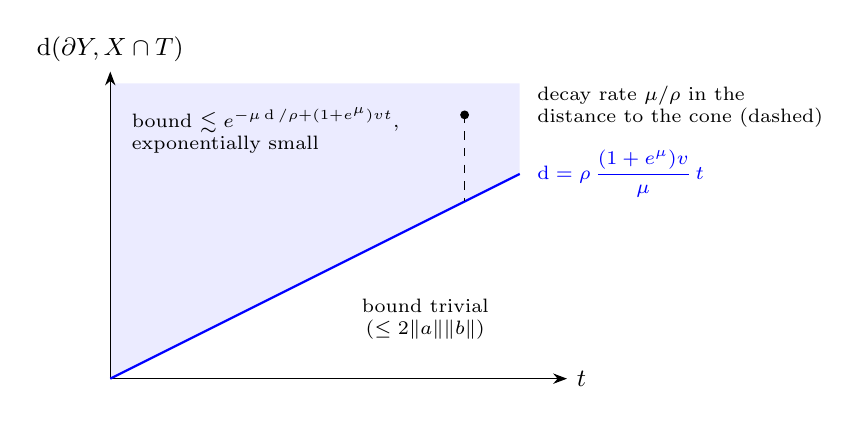
\begin{tikzpicture}[x=1cm,y=1cm,>={Stealth[length=5pt]}]
  \fill[Blue!8] (0,0) -- (5.2,2.6) -- (5.2,3.75) -- (0,3.75) -- cycle;
  \draw[->] (0,0) -- (5.8,0) node[right,font=\small] {$t$};
  \draw[->] (0,0) -- (0,3.9) node[above,font=\small] {$\dist(\bd Y,X\cap T)$};
  \draw[Blue,thick] (0,0) -- (5.2,2.6);
  \node[font=\scriptsize,Blue,anchor=west] at (5.3,2.6) {$\dist=\rho\,\dfrac{(1+e^{\mu})v}{\mu}\,t$};
  \node[font=\scriptsize,align=left,anchor=west] at (0.15,3.15)
    {bound $\lesssim e^{-\mu\dist/\rho+(1+e^{\mu})vt}$,\\ exponentially small};
  \node[font=\scriptsize,align=center] at (4.0,0.75) {bound trivial\\ ($\le2\norm a\norm b$)};
  \fill (4.5,3.35) circle (1.6pt);
  \draw[dashed] (4.5,3.35) -- (4.5,2.25);
  \node[font=\scriptsize,align=left,anchor=west] at (5.3,3.45)
    {decay rate $\mu/\rho$ in the\\ distance to the cone (dashed)};
\end{tikzpicture}

\caption{\vet{The light cone of Theorem~\ref{thm:cone}, for $\mu,\rho>0$: in the plane of the
distance between the probe's boundary and the observable's region against the time $t$, the
bound is at most a constant times $e^{-\mu\,\dist/\rho+(1+e^{\mu})vt}$, so it is small outside
the cone $\dist>\rho(1+e^{\mu})vt/\mu$ (shaded) and trivial inside it. The slope of the line is
schematic. The velocity $(1+e^{\mu})v\rho/\mu$ and the decay rate $\mu/\rho$ are those of the
bound, not of the dynamics.}}
\label{fig:lightcone}
\end{figure}

\begin{theorem}[closed form (iv): the exponential light cone]\label{thm:cone}
\vet{Under the hypotheses of Theorem~\ref{thm:geometry}, for every real $\mu$,
\begin{equation}\label{eq:coneform}
  \norm{\comm{A(t)}b}\le2\norm a\norm b\Bigl(\ind{X\cap Y\ne\emptyset}
  +|\bd Y|\,e^{vt}\,e^{-\mu r}\bigl(e^{e^{\mu}vt}-1\bigr)\Bigr).
\end{equation}}
\end{theorem}

\begin{proof}
\vet{For $r\ge1$ and $x\ge0$, $x^r/r!=e^{-\mu r}(e^{\mu}x)^r/r!\le e^{-\mu r}\sum_{j\ge1}(e^{\mu}x)^j/j!
=e^{-\mu r}(e^{e^{\mu}x}-1)$; insert $x=vt$ into \eqref{eq:geometryform}.}
\end{proof}

\vet{Take $\mu,\rho>0$, regions with $\bd Y$ and $X\cap T$ nonempty, and let
\vetnew{$\dist(\bd Y,X\cap T)$}$:=\min\{d(y,x):y\in\bd Y,\ x\in X\cap T\}$ be positive; put
$r=\lceil\vetnew{\dist(\bd Y,X\cap T)}/\rho\rceil\ge1$. The hypothesis of Theorem~\ref{thm:geometry}
holds, and \eqref{eq:coneform}
is at most a constant times $e^{-\mu\,\vetnew{\dist(\bd Y,X\cap T)}/\rho+(1+e^{\mu})vt}$: a light cone of
velocity $(1+e^{\mu})v\rho/\mu$ with decay rate $\mu/\rho$ outside it
(Figure~\ref{fig:lightcone}).}

\begin{example}[a nearest-neighbour chain]\label{ex:cone}
\vet{Nearest-neighbour terms on the chain $\{0,\dots,n\}$, one term $\{j,j+1\}$ per bond with
$\kappa_j\le\ell$: each site lies in at most $g=2$ supports of size $p=2$ and diameter
$\rho=1$, so $v=8\ell$. For an observable at the site $0$ and a probe at the site $n\ge1$, the
boundary is $\bd Y=\{n\}$ and $r=n$, and Theorem~\ref{thm:geometry} reads
$\norm{\comm{A(t)}b}\le2\norm a\norm b\,(8\ell t)^ne^{8\ell t}/n!$. With $\mu=1$,
Theorem~\ref{thm:cone} gives a light cone of velocity $(1+e)\cdot8\ell\approx30\ell$ and decay
rate $1$ per site outside it. The velocity is an artefact of the walk bound; on the three-site
chain of Example~\ref{ex:chain} the path series itself is sharp to leading order at short
times.}
\end{example}

\subsection{Time reversal}\label{subsec:reversal}

\vet{We proved the path-sum bound for $t\ge0$, because hypothesis (G3) is a statement about
$e^{tL_J}$ for $t\ge0$. If the family also satisfies (G3) with every $L_i$ replaced by $-L_i$,
which is the case for a group of automorphisms, \revs{we say that the family has a
\emph{contractive negation}, and then} the bound holds for all times.}

\begin{theorem}[time reversal]\label{thm:reverse}
\vet{Let the net be causal, and suppose $\norm{e^{-tL_J}}\le1$ for every $J\subseteq I$ and
$t\ge0$. Then \eqref{eq:master}, \eqref{eq:walkseries} and \eqref{eq:decayform} hold for every
$t\in\R$ with $|t|$ in place of \vetnew{$t$.}}
\end{theorem}

\begin{proof}
\vet{The negated family $(S_i,-L_i,\kappa_i)$ satisfies (G1) and (G2), since
$\norm{-L_ic}=\norm{L_ic}$ and $\cA(Z\cup S_i)$ is a subspace, and (G3) by hypothesis; it has the
same supports and strengths, hence the same paths, counts, site matrix and walk weights, and its
dynamics at time $|t|$ is $e^{|t|(-L)}=e^{tL}$ for $t<0$. Apply the bounds to it.}
\end{proof}

\vetnew{The matrix form \eqref{eq:matrixform} and the bounded-geometry and light-cone forms
\eqref{eq:geometryform} and \eqref{eq:coneform} follow from \eqref{eq:walkseries} alone, by the
proofs of Proposition~\ref{prop:finite} and Theorems~\ref{thm:geometry} and~\ref{thm:cone}.
Applied to the negated family, which has the same supports and strengths, they too hold for every
$t\in\R$ with $|t|$ in place of $t$ under the hypothesis of Theorem~\ref{thm:reverse}.}

\subsection*{Notes and references}
\vet{\emph{Site matrix.} The review \cite{chen-lucas-yin} defines $h_{uu'}$ for two-site terms,
with $\norm{H_{uu'}}$ off the diagonal and the sum of the strengths at a site on it (its
eq.~(3.35)); \cite{chen-lucas2021} writes $h_{ij}=\sum_{X\ni i,j}\norm{H_X}$ for general
supports. Definition~\ref{def:sitematrix} is the latter with $\kappa_i$ in place of $\norm{H_X}$,
and \eqref{eq:matrixform} is \vetnew{the review's (3.36), with its constant doubled and the $-1$
that the series proof gives}; the review's commutator quantity is half of $C_{X,Y}(t)$.

\emph{Boundary and decay functions.} The boundary $\bd Y$ is the $\Phi$-boundary of
\cite{nsy2019}, eq.~(3.20). Decay functions $F_0$ with a reproducing constant and the $F$-norm
are \cite{nsy2019}, eqs.~(3.8)--(3.9) and (3.14); \vetnew{Theorem~3.1 of \cite{nsy2019}} is \eqref{eq:decayform}
with $F=F_0\circ d$ and $N_F$ the $F$-norm, the exponent $2N_FC_Ft$ being their $2I_{t,s}$ for a
time-independent interaction. Only the finite-sum form \eqref{eq:reproducing} enters here, so
neither a metric nor the convergence of $\sum_yF_0(d(x,y))$ is needed before
Chapter~\ref{sec:qudit}.

\emph{Geometry.} The bounded-degree form is the review's Proposition~3.5, whose constants
($4(g-1)h$ for the velocity and $K=1/(1-2/e)$ for the tail) are sharper than
\eqref{eq:geometryform}'s $v=2g\ell p$ and $e^{vt}$, because the review's walks never return
along the edge they came from; the exponential form is \vetnew{the review's Example~3.6}.}

\paragraph{Checks.} {\small The site matrix, walk weights and series of
Example~\ref{ex:chainwalk}, the domination on random hypergraphs, the constants $C_F$ (the least
constant on a chain of $40$ sites at $\lambda=\tfrac12$ is $3.72$) and $N_F=4e^{\lambda}$ of
Example~\ref{ex:kernel}, the vanishing of $(h^k)_{xy}$ below the distance, the tail bound behind
Example~\ref{ex:cone} and the comparison with the review's Proposition~3.5 are computed by
\texttt{checks/m1b\_check.py}.}


\clearpage
\section{Hamiltonians and qudit lattices}\label{sec:qudit}

\motiv{\vet{We stated the theorem of Chapter~\ref{sec:master} for bounded generators with three
properties, and Example~\ref{ex:hamiltonian} sketched why Hamiltonian terms have them. This
chapter proves it once for all. A Hamiltonian built from self-adjoint local terms $\Phi_i$ generates the derivations
$a\mapsto\ii\comm{\Phi_i}a$, and the three properties are three facts about a C*-algebra:
locality in the argument is the homogeneity of the commutator seminorm, support closure is
isotony, and contraction, in both time directions, is the unitarity of $e^{\ii tH}$. The
dynamics is then the familiar conjugation $A(t)=e^{\ii tH}ae^{-\ii tH}$, which we compute rather
than postulate, and one more line, the role exchange of the observable and the probe, lets the
bound be read from the observable's boundary as well as from the probe's, and the smaller
reading taken.

The second half of the chapter builds the net on which spin systems live: a finite set of
sites, each carrying a finite alphabet, the matrix algebra on the configurations, and the local
algebra of a region, defined by what its matrices do to configurations rather than by a tensor
product. The published bounds for spin systems are then corollaries, and a two-qubit example
shows that the dynamics they bound is not trivial.}}

\subsection{Hamiltonian families}

\vet{Throughout the first half, $\cA$ is a unital C*-algebra, nontrivial ($1\ne0$, so that a
unitary has norm one), with a causal net $Z\mapsto\cA(Z)$ over the subsets of a set of sites
$\Lambda$ (Definition~\ref{def:net}). For $x\in\cA$ write $\mathrm L_x:a\mapsto xa$ and
$\mathrm R_x:a\mapsto ax$ for the left and right multiplications, bounded operators on $\cA$ of
norm at most $\norm x$, and
\begin{equation}\label{eq:ad}
  \ad_x:a\longmapsto\ii(xa-ax)=\ii\comm xa,
\end{equation}
the \emph{derivation} of $x$; $\ad$ is linear in $x$ and $\norm{\ad_x}\le2\norm x$.}

\begin{definition}[Hamiltonian family]\label{def:hamfamily}
\vet{A \emph{Hamiltonian family} on the net is a finite family $(S_i,\Phi_i)_{i\in I}$ of finite
supports $S_i\subseteq\Lambda$ and self-adjoint elements $\Phi_i\in\cA(S_i)$. For $J\subseteq I$
put $H_J:=\sum_{i\in J}\Phi_i$, and $H:=H_I$. The generators of the family are $L_i:=\ad_{\Phi_i}$,
so that $L_J=\sum_{i\in J}L_i=\ad_{H_J}$ and $L=\ad_H$.}
\end{definition}

\vet{In the language of the sources the family is an \emph{interaction}, a map from finite sets
to self-adjoint local elements; we index it by a finite set so that one support may carry
several terms, as in Chapter~\ref{sec:objects}.}

\begin{proposition}[the derivation is a local generator]\label{prop:derivation}
\vet{Let $x\in\cA(S)$ and $c\in\cA$.
\begin{enumerate}[label=(\alph*),nosep]
\item $\norm{\ad_x c}\le\norm x\,N_S(c)$: locality in the argument holds with $\kappa=\norm x$.
\item If $c\in\cA(Z)$ then $\ad_x c\in\cA(Z\cup S)$: support closure.
\end{enumerate}}
\end{proposition}

\begin{proof}
\vet{\begin{enumerate}[label=(\alph*),nosep]
\item If $x=0$ there is nothing to prove. Otherwise $b:=x/\norm x$ lies in $\cA(S)$ with
$\norm b=1$, and $\ad_xc=-\ii\norm x\comm cb$, so $\norm{\ad_xc}=\norm x\norm{\comm cb}
\le\norm x\,N_S(c)$ by the definition of the seminorm.
\item By isotony both $x$ and $c$ lie in $\cA(Z\cup S)$, which is closed under products,
differences and scalars.\qedhere
\end{enumerate}}
\end{proof}

\vet{The third hypothesis, contraction of every sub-family, is unitarity. To see it we compute the
exponential of a derivation. The computation rests on a small fact about multiplications.}

\begin{proposition}[exponential of a multiplication]\label{prop:expmul}
\vet{For $x,y\in\cA$: $\exp(\mathrm L_x)=\mathrm L_{\exp x}$, $\exp(\mathrm R_y)=\mathrm R_{\exp y}$,
the operators $\mathrm L_x$ and $\mathrm R_y$ commute, and
\begin{equation}\label{eq:expmul}
  \exp(\mathrm L_x+\mathrm R_y)\,a=e^{x}\,a\,e^{y}\qquad(a\in\cA).
\end{equation}}
\end{proposition}

\begin{proof}
\vet{$\mathrm L_x^{\,k}=\mathrm L_{x^k}$, and $x\mapsto\mathrm L_x$ is a bounded linear map, so
it commutes with the convergent exponential series: $\exp(\mathrm L_x)=\sum_k\mathrm L_{x^k}/k!
=\mathrm L_{\exp x}$. The same for $\mathrm R_y$. Commutation is associativity, $(xa)y=x(ay)$.
For commuting bounded operators $P,Q$ on a Banach space, $\exp(P+Q)=\exp P\exp Q$ (the
binomial rearrangement of the absolutely convergent series), and
$\mathrm L_{e^x}\mathrm R_{e^y}a=e^xae^y$.}
\end{proof}

\begin{proposition}[unitary conjugation]\label{prop:conjugation}
\vet{Let $H\in\cA$ be self-adjoint and $t\in\R$. Then $U_t:=\exp(\ii tH)$ is unitary with
$U_t^*=\exp(-\ii tH)=U_{-t}$, and
\begin{equation}\label{eq:conjugation}
  \exp(t\,\ad_H)\,a=U_t\,a\,U_t^*,\qquad\norm{\exp(t\,\ad_H)\,a}=\norm a\qquad(a\in\cA).
\end{equation}}
\end{proposition}

\begin{proof}
\vet{The adjoint commutes with the exponential series, so $U_t^*=\exp((\ii tH)^*)=\exp(-\ii tH)$,
and $\ii tH$ commutes with $-\ii tH$, so $U_t^*U_t=\exp(0)=1=U_tU_t^*$: $U_t$ is unitary. On $a$,
$t\,\ad_Ha=\ii tHa-a\,\ii tH=(\mathrm L_{\ii tH}+\mathrm R_{-\ii tH})a$, and
Proposition~\ref{prop:expmul} gives $\exp(t\ad_H)a=e^{\ii tH}ae^{-\ii tH}$. Multiplication by a
unitary on either side preserves the norm: $\norm{Ua}^2=\norm{a^*U^*Ua}=\norm a^2$ by the
C*-identity, and $\norm{aU}=\norm{(aU)^*}=\norm{U^*a^*}=\norm{a^*}=\norm a$ since $U^*$ is
unitary too.}
\end{proof}

\begin{theorem}[Hamiltonian families are local generators]\label{thm:hamgenerators}
\vet{A Hamiltonian family $(S_i,\Phi_i)_{i\in I}$ defines the family of local generators
$(S_i,\ad_{\Phi_i},\norm{\Phi_i})_{i\in I}$ of Definition~\ref{def:local-generators}, and its
negation is contractive as well. The dynamics is
\begin{equation}\label{eq:hamdynamics}
  A(t)=e^{tL}a=U_t\,a\,U_t^*,\qquad U_t=e^{\ii tH},\quad t\in\R .
\end{equation}
Consequently \vetnew{the path-sum bound \eqref{eq:master}, the walk series \eqref{eq:walkseries}
and the decay form \eqref{eq:decayform} hold for every Hamiltonian family at every $t\in\R$ with
$|t|$ in place of $t$ (Theorem~\ref{thm:reverse}),} with $\kappa_i=\norm{\Phi_i}$.}
\end{theorem}

\begin{proof}
\vet{G1 and G2 are Proposition~\ref{prop:derivation}. For G3 fix $J$ and $t\ge0$: $L_J=\ad_{H_J}$
with $H_J$ self-adjoint, so $\norm{e^{tL_J}a}=\norm a$ for all $a$ by
Proposition~\ref{prop:conjugation}, that is $\norm{e^{tL_J}}\le1$; at $-t$ the same gives G3 for
the negated family. The formula is Proposition~\ref{prop:conjugation} with $J=I$.}
\end{proof}

\vetnew{The other closed forms of Chapter~\ref{sec:closed}, the matrix form on a finite lattice
and the bounded-geometry and light-cone forms, hold for a Hamiltonian family as for every family
of local generators for $t\ge0$, and for every $t\in\R$ with $|t|$ in place of $t$ by the
paragraph after Theorem~\ref{thm:reverse}.}

\vet{The sources define the dynamics through the Schrödinger equation of a propagator and prove
unitarity from it; here the dynamics is $e^{tL}$, as in Chapter~\ref{sec:master}, and the
conjugation form is a computation.}

\subsection{Role exchange}

\vet{The path-sum bound treats the observable and the probe asymmetrically: the walks of
Chapter~\ref{sec:closed} start on the boundary $\bd Y$ of the probe's region. For an
automorphism group we can exchange the two roles, and the bound improves to the smaller of the
two readings. Theorem~3.1 of \cite{nsy2019} carries this minimum, written $D(X,Y)$ in their
eq.~(3.24): the smaller of the \vetnew{sums of the decay function} over $\bd Y\times X$ and over $\bd X\times Y$; their
proof obtains the second from the same one-line identity, their eq.~(3.39). Below, $B(t):=e^{tL}b$
is the evolved probe, and $T$, $\bd$, $W_k$ are those of Chapter~\ref{sec:closed}.}

\needspace{16\baselineskip}
\begin{theorem}[role exchange]\label{thm:exchange}
\vet{For a unitary $U$ and $a,b\in\cA$,
\begin{equation}\label{eq:exchange}
  \comm{UaU^*}b=U\comm a{U^*bU}U^*,\qquad\text{hence}\qquad
  \norm{\comm{UaU^*}b}=\norm{\comm a{U^*bU}} .
\end{equation}
For a Hamiltonian family, $a\in\cA(X)$, $b\in\cA(Y)$ and $t\in\R$,
$\norm{\comm{A(t)}b}=\norm{\comm{B(-t)}a}$, and
\begin{equation}\label{eq:exchangewalk}
  \norm{\comm{A(t)}b}\le2\norm a\norm b\Bigl(\ind{X\cap Y\ne\emptyset}
  +\min\Bigl\{\sum_{k\ge1}\frac{(2|t|)^k}{k!}W_k(Y,X),\ \sum_{k\ge1}\frac{(2|t|)^k}{k!}W_k(X,Y)\Bigr\}\Bigr),
\end{equation}
where $W_k(X,Y)$ sums the walks from $\bd X$ to $Y\cap T$. The decay form of
Theorem~\ref{thm:decay} holds likewise with $\min\{\Sigma_F(Y,X),\Sigma_F(X,Y)\}$.}
\end{theorem}

\begin{proof}
\vet{$\comm{UaU^*}b=UaU^*b-bUaU^*=U(aU^*bU-U^*bUa)U^*$ since $U^*U=1$; conjugation preserves
the norm. With $U=U_t$, $U^*bU=U_{-t}bU_{-t}^*=B(-t)$ by \eqref{eq:hamdynamics}. The first
series is the time-reversed walk bound (Theorem~\ref{thm:reverse}); the second is the same
bound at time $-t$ for the pair $(b,a)$, whose regions are $(Y,X)$, and $|-t|=|t|$. The smaller of
two upper bounds is an upper bound; the minimum is of the two sums, not of their terms.}
\end{proof}

\subsection{Qudit lattices}\label{subsec:qudit-lattices}

\vet{Now let $\Lambda$ be a finite set of sites, each carrying a finite nonempty alphabet
$\Omega_u$; a \emph{qudit} of dimension $n$ is the alphabet $\{0,\dots,n-1\}$ at every site. A
\emph{configuration} is a choice $s=(s(u))_{u\in\Lambda}$ of a letter at each site; there are
finitely many. The \emph{qudit algebra} $\Mat_\Lambda$ is the algebra of complex matrices indexed
by configurations, with the operator norm of $\ell^2$ over the configurations; it is a
C*-algebra. For a region $X$ write $s|_X$ for the restriction of $s$ to $X$, and $s\sim_Xs'$
when $s$ and $s'$ agree at every site outside $X$, that is, $s|_{X^c}=s'|_{X^c}$, and, for a
choice $\xi$ of letters on $X$,
$(\xi,s|_{X^c})$ for the configuration equal to $\xi$ on $X$ and to $s$ off $X$
(Figure~\ref{fig:configsplit}).}

\begin{figure}[htb]
\centering
% Figure: a configuration of a chain of six sites split by a region X = {2, 3}. Transcription
% (for cheap agents): six sites 0..5 on a line, each carrying a letter of the alphabet {0, 1}
% written in a small box above the site: s = (1, 0, 0, 1, 1, 0); the region X = {2, 3} is a
% dashed box around sites 2 and 3; the part on X, s|_X = (0, 1), is shaded blue; the part off X,
% (1, 0, ., ., 1, 0), is left white. Below, a second configuration s' = (1, 0, 1, 1, 1, 0) with the
% same letters off X and different letters on X, labelled "s ~_X s'" and "s' = (xi, s|_{X^c}) with
% xi = (1, 1)". The caption explains that a matrix local to X has an entry at (s, s') only when
% the two configurations agree off X, and that the entry depends on the shaded parts alone.
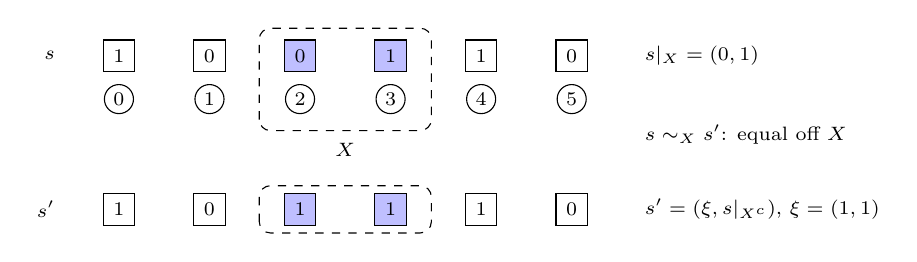
\begin{tikzpicture}[x=1.15cm,y=1cm,
  site/.style={circle,draw,fill=white,inner sep=1.6pt,font=\scriptsize},
  letter/.style={draw,rectangle,inner sep=2pt,minimum size=0.4cm,font=\scriptsize},
  onX/.style={draw,rectangle,inner sep=2pt,minimum size=0.4cm,font=\scriptsize,fill=Blue!25},
  region/.style={rounded corners=4pt,draw,dashed,fill=none},
  lab/.style={font=\scriptsize}]
  % configuration s
  \node[lab,anchor=east] at (-0.6,0.55) {$s$};
  \foreach \u/\l in {0/1,1/0,4/1,5/0} { \node[letter] at (\u,0.55) {\l}; }
  \node[onX] at (2,0.55) {0}; \node[onX] at (3,0.55) {1};
  \foreach \u in {0,...,5} { \node[site] at (\u,0) {\u}; }
  \draw[region] (1.55,-0.4) rectangle (3.45,0.9);
  \node[lab] at (2.5,-0.65) {$X$};
  % configuration s'
  \node[lab,anchor=east] at (-0.6,-1.4) {$s'$};
  \foreach \u/\l in {0/1,1/0,4/1,5/0} { \node[letter] at (\u,-1.4) {\l}; }
  \node[onX] at (2,-1.4) {1}; \node[onX] at (3,-1.4) {1};
  \draw[region] (1.55,-1.7) rectangle (3.45,-1.1);
  \node[lab,anchor=west] at (5.7,0.55) {$s|_X=(0,1)$};
  \node[lab,anchor=west] at (5.7,-1.4) {$s'=(\xi,s|_{X^c})$, $\xi=(1,1)$};
  \node[lab,anchor=west] at (5.7,-0.45) {$s\sim_Xs'$: equal off $X$};
\end{tikzpicture}

\caption{\vet{Two configurations of a chain of six sites with the alphabet $\{0,1\}$, split by
the region $X=\{2,3\}$. They agree off $X$ (the white boxes), so $s\sim_Xs'$, and $s'$ is
$(\xi,s|_{X^c})$ for the letters $\xi=(1,1)$ on $X$. A matrix local to $X$ has a nonzero entry at
$(s,s')$ only for such pairs, and the entry depends on the shaded parts $s|_X$, $s'|_X$ alone
(Definition~\ref{def:localmatrix}).}}
\label{fig:configsplit}
\end{figure}

\begin{definition}[local algebra]\label{def:localmatrix}
\vet{A matrix $M\in\Mat_\Lambda$ is \emph{local to $X$} if
\begin{enumerate}[label=(\arabic*),nosep]
\item $M_{ss'}=0$ whenever $s\not\sim_Xs'$, and
\item $M_{ss'}=M_{rr'}$ whenever $s\sim_Xs'$, $r\sim_Xr'$, $s|_X=r|_X$ and $s'|_X=r'|_X$.
\end{enumerate}
$\cA(X)$ is the set of matrices local to $X$. For a matrix $m$ on the letters of $X$, its
\emph{embedding} $\iota_Xm$ is the matrix $(\iota_Xm)_{ss'}:=\ind{s\sim_Xs'}\,m_{s|_X,s'|_X}$ (the
tensor factor $m\otimes1$ of the sources).}
\end{definition}

\vet{Condition (1) says that $M$ does not change the letters outside $X$; condition (2) that
what it does inside $X$ does not depend on the letters outside. Together they say that $M$ acts
on the part inside $X$ and as the identity outside, which is what $m\otimes1$ means in the
tensor-product picture; the definition avoids the tensor product and keeps every proof an entry
computation. The embedded matrices are exactly the local ones.}

\begin{lemma}[sum over a class]\label{lem:glue}
\vet{For a configuration $s$ and a function $f$ of configurations that vanishes off the class of
$s$ (that is, $f(s')=0$ unless $s'\sim_Xs$),
\begin{equation}\label{eq:glue}
  \sum_{s'}f(s')=\sum_{\xi}f(\xi,s|_{X^c}),
\end{equation}
the right side summing over the choices of letters on $X$.}
\end{lemma}

\begin{proof}
\vet{$\xi\mapsto(\xi,s|_{X^c})$ is a bijection from the letters on $X$ onto the class of $s$,
with inverse $s'\mapsto s'|_X$; re-index the sum, dropping the vanishing terms.}
\end{proof}

\needspace{10\baselineskip}
\begin{proposition}[local algebras]\label{prop:localalgebra}
\begin{enumerate}[label=(\alph*),nosep]
\item \vet{$\cA(X)$ is a star subalgebra of $\Mat_\Lambda$ containing $1$, and it is closed.}
\item \vet{$\iota_Xm\in\cA(X)$, and every $M\in\cA(X)$ is $\iota_Xm$ for \vetnew{some matrix
  $m$ on the letters of $X$}.}
\item \vet{If $X\subseteq Y$ then $\cA(X)\subseteq\cA(Y)$; and $\cA(\Lambda)=\Mat_\Lambda$.}
\end{enumerate}
\end{proposition}

\begin{proof}
\vet{\begin{enumerate}[label=(\alph*),nosep]
\item Both conditions are linear in $M$, hold for $1$ (equal configurations agree off $X$, and
for $s\sim_Xs'$ the equality $s=s'$ is decided by $s|_X=s'|_X$), and are symmetric under
$(s,s')\mapsto(s',s)$, which handles the adjoint. For the product let $M,N\in\cA(X)$. If
$s\not\sim_Xs''$, every term $M_{ss'}N_{s's''}$ vanishes, since $M_{ss'}\ne0$ forces $s'\sim_Xs$
and $N_{s's''}\ne0$ forces $s''\sim_Xs'$. If $s\sim_Xs''$, Lemma~\ref{lem:glue} gives
$(MN)_{ss''}=\sum_\xi M_{s,(\xi,s|_{X^c})}N_{(\xi,s|_{X^c}),s''}$, and each factor is unchanged
when $(s,s'')$ is replaced by $(r,r'')$ with $r\sim_Xr''$ and the same parts on $X$, by
condition (2). Closedness: a subspace of a finite-dimensional space.
\item The embedding satisfies (1) by its indicator and (2) because its entries depend on the
parts on $X$ only. Conversely, \vetnew{fix a configuration $s_0$, which exists as the alphabets
are nonempty, and put $m_{\xi\eta}:=M_{(\xi,s_0|_{X^c}),(\eta,s_0|_{X^c})}$. For} $s\sim_Xs'$
condition (2) with $r=(s|_X,s_0|_{X^c})$,
$r'=(s'|_X,s_0|_{X^c})$ gives $M_{ss'}=m_{s|_X,s'|_X}$, and both sides vanish otherwise.
\item If $s\not\sim_Ys'$ then $s\not\sim_Xs'$. For (2), if $s\sim_Xs'$ then $r\sim_Xr'$, because
off $Y$ the pair $(r,r')$ agrees and on $Y\setminus X$ it copies $(s,s')$, which agrees there;
the restrictions to $X$ agree, so condition (2) for $X$ applies. If $s\not\sim_Xs'$ then
likewise $r\not\sim_Xr'$ and both entries vanish. For $X=\Lambda$ both conditions are empty.\qedhere
\end{enumerate}}
\end{proof}

\begin{theorem}[the qudit net is causal]\label{thm:quditnet}
\vet{$X\mapsto\cA(X)$ is a net over the subsets of $\Lambda$, and local matrices of disjoint
regions commute: $M\in\cA(X)$, $N\in\cA(Y)$ and $X\cap Y=\emptyset$ give $MN=NM$.}
\end{theorem}

\begin{proof}
\vet{Fix $s,s''$. A term $M_{ss'}N_{s's''}$ is nonzero only if $s'$ agrees with $s$ off $X$ and
with $s''$ off $Y$; as $X\cap Y=\emptyset$ this determines $s'$: on $X$ it equals $s''$, elsewhere
$s$. Call it $\bar s$; then $(MN)_{ss''}=M_{s\bar s}N_{\bar ss''}$. Likewise
$(NM)_{ss''}=N_{s\hat s}M_{\hat ss''}$ with $\hat s$ equal to $s''$ on $Y$ and to $s$ elsewhere.
If $s$ and $s''$ differ somewhere off $X\cup Y$, then $\bar s\not\sim_Ys''$ and $\hat s\not\sim_Xs''$,
so both products vanish. Otherwise $M_{s\bar s}=M_{\hat ss''}$ by condition (2) for $X$
($s\sim_X\bar s$, $\hat s\sim_Xs''$, $s|_X=\hat s|_X$, $\bar s|_X=s''|_X$) and
$N_{\bar ss''}=N_{s\hat s}$ by (2) for $Y$, and the two products agree.}
\end{proof}

\vet{Two further constructions serve the examples; both are for a
uniform alphabet $\Omega$. For a matrix $m$ on $\Omega$ and a site $u$, the \emph{single-site
operator} $m_u$ acts by $m$ at the site $u$ and trivially elsewhere,
$(m_u)_{ss'}=\ind{s\sim_{\{u\}}s'}m_{s(u),s'(u)}$, the usual notation $\sigma^x_u$ for a Pauli
matrix at a site. It is local to $\{u\}$ (we read both conditions off the formula);
$m_um'_u=(mm')_u$, because the configurations agreeing with $s$ off $u$ are parametrized by
their letter at $u$, so the sum over them is the matrix product at $(s(u),s''(u))$; operators at
distinct sites commute by Theorem~\ref{thm:quditnet}; and for $u\ne v$ and $s\sim_{\{u,v\}}s''$
the one nonzero term of the product gives $(m_um'_v)_{ss''}=m_{s(u),s''(u)}m'_{s(v),s''(v)}$. A
bijection
$\varphi:\Lambda\to\Lambda'$ of site sets, both with the alphabet $\Omega$, induces the
star-isomorphism $M\mapsto M^\varphi$ of the qudit algebras,
$(M^\varphi)_{rr'}:=M_{r\circ\varphi,\,r'\circ\varphi}$ for configurations $r,r'$ of $\Lambda'$
(re-indexing along the bijection $r\mapsto r\circ\varphi$ of configurations, which commutes with
products and adjoints); it carries $\cA(X)$ onto $\cA(\varphi(X))$, since
$r\sim_{\varphi(X)}r'$ iff $r\circ\varphi\sim_Xr'\circ\varphi$ and $r|_{\varphi(X)}$ determines
$(r\circ\varphi)|_X$ and conversely, so that $M$ is local to $X$ iff $M^\varphi$ is local to
$\varphi(X)$, and $\varphi^{-1}$ gives the inverse. This is the covariance a
translation-invariant system on a finite torus needs. \vetnew{On two qubits, $\sigma^x_1$ is not local
to $\{0\}$: the configurations $00$ and $01$ (the letter at the site $0$ written first) differ
at the site $1$, outside $\{0\}$, yet the entry of $\sigma^x_1$ between them is $1$, against
condition~(1). And $\sigma^x_0$, $\sigma^z_0$ do not commute: the net is not trivial.}}

\subsection{The bounds for spin systems}

\begin{definition}[qudit interaction]\label{def:quditinteraction}
\vet{A \emph{qudit interaction} is a finite family $(S_i,m_i)_{i\in I}$ of finite supports and
Hermitian matrices $m_i$ on the letters of $S_i$; its terms $\Phi_i:=\iota_{S_i}m_i$
are self-adjoint and local to $S_i$, so the family is a Hamiltonian family on the qudit net.}
\end{definition}

\needspace{10\baselineskip}
\begin{theorem}[the published bounds for qudits]\label{thm:quditbounds}
\vet{For a qudit interaction, $a\in\cA(X)$, $b\in\cA(Y)$, with the site matrix $h$ of the
strengths $\kappa_i=\norm{\Phi_i}$:
\begin{enumerate}[label=(\roman*),nosep]
\item for all $t\in\R$, the walk bound \eqref{eq:exchangewalk}, and on the finite lattice
  \begin{equation}\label{eq:quditmatrix}
    \norm{\comm{A(t)}b}\le2\norm a\norm b\Bigl(\ind{X\cap Y\ne\emptyset}
    +\sum_{y\in\bd Y}\sum_{x\in X\cap T}\bigl(e^{2|t|h}-1\bigr)_{yx}\Bigr),
  \end{equation}
  and the same with the roles exchanged, the sum over $\bd X\times(Y\cap T)$;
\item for a \vetnew{decay function} $(F,C_F)$ and an $F$-bound $N_F$, for all $t\in\R$,
  \begin{equation}\label{eq:quditdecay}
    \norm{\comm{A(t)}b}\le2\norm a\norm b\Bigl(\ind{X\cap Y\ne\emptyset}
    +\frac{e^{2N_FC_F|t|}-1}{C_F}\min\{\Sigma_F(Y,X),\Sigma_F(X,Y)\}\Bigr);
  \end{equation}
\item with bounded geometry, for $t\ge0$ as stated there, the forms \eqref{eq:geometryform} and
  \eqref{eq:coneform} of Chapter~\ref{sec:closed}.
\end{enumerate}}
\end{theorem}

\begin{proof}
\vet{Theorem~\ref{thm:hamgenerators} puts the interaction, on the causal net of
Theorem~\ref{thm:quditnet}, under the hypotheses of Chapter~\ref{sec:closed} with a contractive
negation; (i) and (ii) are the time-reversed forms with Theorem~\ref{thm:exchange}, the matrix
form by Proposition~\ref{prop:finite} at $|t|$, (iii) the geometric forms.}
\end{proof}

\vet{\vetnew{Equation~\eqref{eq:quditmatrix} is the review's (3.36) \cite{chen-lucas-yin}, with its
constant doubled and the $-1$ that the series proof gives (the review's $\mathcal C$ is half the
supremum, and the identity has no entry between distinct sites), and with the sum restricted to
$\bd Y\times(X\cap T)$;}
\eqref{eq:quditdecay} is Theorem~3.1 of \cite{nsy2019} for time-independent interactions, whose
boundary $\bd_\Phi$ is $\bd$ when each support carries one nonzero term. Two further facts
connect the \vetnew{decay functions} of Chapter~\ref{sec:closed} to the sources' $F$-functions. In
them, \vetnew{$d$ is a distance on $\Lambda$ as in Definition~\ref{def:geometry} ($d(u,u)=0$ and
the triangle inequality, not assumed symmetric)}, and $T'$ ranges over the finite subsets of
$\Lambda$.}

\begin{proposition}[the $F$-norm; weighted decay functions]\label{prop:fnorm}
\begin{enumerate}[label=(\alph*),nosep]
\item \vet{For \vetnew{a decay function $F>0$ on the finite nonempty set $\Lambda$},
  $\norm\Phi_F:=\max_{x,y}h_{xy}/F(x,y)$ is an $F$-bound, and every $F$-bound $N$ satisfies
  $N\ge\norm\Phi_F$.}
\item \vet{If $(F,C_F)$ is a \vetnew{decay function} and $d$ satisfies the triangle inequality, then for
  $\mu\ge0$ the \vetnew{\emph{weighted decay function}} $F_\mu(x,y):=e^{-\mu d(x,y)}F(x,y)$ is a
  \vetnew{decay function} with
  the same constant $C_F$ (the weighted $F$-functions of \cite{nsy2019}, eq.~(3.11), for the
  weight $\mu r$).}
\end{enumerate}
\end{proposition}

\begin{proof}
\vet{\begin{enumerate}[label=(\alph*),nosep]
\item A maximum dominates each value, and $F>0$ clears the denominator; conversely
$h_{xy}/F(x,y)\le N$ for every pair bounds the maximum.
\item $e^{-\mu(d(x,z)+d(z,y))}\le e^{-\mu d(x,y)}$ for $\mu\ge0$, so
\[
\sum_{z\in T'}F_\mu(x,z)F_\mu(z,y)\le e^{-\mu d(x,y)}\sum_{z\in T'}F(x,z)F(z,y)\le C_FF_\mu(x,y).\qedhere
\]
\end{enumerate}}
\end{proof}

\vetnew{With $F(x,y)=F_0(d(x,y))$ and one term per support, the number $\norm\Phi_F$ of (a) is
the $F$-norm $\sup_{x,y}F_0(d(x,y))^{-1}\sum_{Z\ni x,y}\norm{\Phi(Z)}$ of \cite{nsy2019},
eq.~(3.14); with several terms on a support, $h$ adds their norms.}

\vet{\vetnew{The polynomial decay function $F=F_0\circ d$ with $F_0(r)=(1+r)^{-\alpha}$ on
$\Z^\nu$ with the $\ell^1$ distance has $C_F\le2^\alpha\norm F$ for $\alpha>\nu$, where
$\norm F=\sup_x\sum_yF(x,y)$}; this is
eq.~(3.13) of \cite{nsy2019}, quoted here and not derived (the elementary estimate
$(1+d(x,z))(1+d(z,y))\ge\tfrac12(1+d(x,y))(1+\min\{d(x,z),d(z,y)\})$ gives $2^{\alpha+1}\norm F$).
A finite piece of the lattice inherits the \vetnew{decay function} with a constant at most that of
the lattice. With (b) the \vetnew{weighted decay function} $F_\mu$ gives the exponential light cone of \eqref{eq:quditdecay} at the
velocity $2N_{F_\mu}C_F/\mu$, with $N_{F_\mu}$ an $F_\mu$-bound. On a chain of $20$ sites at
$\alpha=2$ the least reproducing constant is $4.20$ against $2^\alpha\norm F=8.43$; on a
$6\times6$ grid at $\alpha=3$ it is $4.46$ against $16.3$.}

\subsection{Two qubits}

\begin{example}[the exact commutator]\label{ex:twoqubit}
\vet{Two qubits, with the Pauli matrices $\sigma^x=\begin{psmallmatrix}0&1\\1&0\end{psmallmatrix}$,
$\sigma^y=\begin{psmallmatrix}0&-\ii\\\ii&0\end{psmallmatrix}$,
$\sigma^z=\begin{psmallmatrix}1&0\\0&-1\end{psmallmatrix}$ at the sites, $\sigma^x_u$ and so on.
Let $H=\sigma^x_0\sigma^x_1$ (the single term with support $\{0,1\}$ and norm $1$),
$a=\sigma^z_0$, $b=\sigma^z_1$. Since $H^2=1$ and $H$ anticommutes with $a$,
\[
  A(t)=e^{\ii tH}ae^{-\ii tH}=a\,e^{-2\ii tH}=a(\cos2t-\ii\sin2t\,H),\qquad
  \comm{A(t)}b=-2\ii\sin2t\;\sigma^y_0\sigma^y_1,
\]
so $\norm{\comm{A(t)}b}=2|\sin2t|$. The bound \eqref{eq:quditmatrix} has
$h=\begin{psmallmatrix}1&1\\1&1\end{psmallmatrix}$, $\bd Y=\{1\}$, $X\cap T=\{0\}$ and
$(e^{2th}-1)_{10}=(e^{4t}-1)/2$, hence $\norm{\comm{A(t)}b}\le e^{4t}-1$: the ratio of the bound
to the exact norm is $1.24$ at $t=0.1$, $2.05$ at $t=0.3$ and $11.1$ at $t=\pi/4$, where the
commutator is largest. The bound is a bound on growth, not on the oscillation that follows.
\vetnew{The system is that of Example~\ref{ex:twosites} with $\sigma^x$ and $\sigma^z$
exchanged; as there, the path-sum bound of Chapter~\ref{sec:master} gives $4t$ for it, while the
walk bound gives $e^{4t}-1$, the price of counting walks in place of paths.}}
\end{example}

\vet{A second route to the same conclusion, that the dynamics bounded in this chapter is not
trivial, avoids the exponential: at $t=0$ the commutator vanishes by causality, and its
derivative there is \vetnew{$\comm{\ii\comm Ha}b=\ii\,c_0c_1$, the product of the single-site
operators of the matrix $c=\sigma^x\sigma^z-\sigma^z\sigma^x=-2\ii\sigma^y$ at the sites $0$
and $1$. By the product formula for single-site operators, its entry at the row configuration
$00$ and the column configuration $11$ is $\ii\,c(0,1)\,c(0,1)=4\ii\ne0$, where $c(0,1)$ is
the entry of the $2\times2$ matrix $c$ in the row $0$ and the column $1$.} A function vanishing at $0$
with a nonzero derivative there is nonzero at some $t>0$; hence there is $t>0$ with
$\comm{A(t)}b\ne0$.}

\subsection*{Notes and references}
\vetnew{\emph{The review's bound for spin systems.} For edge Hamiltonians $H_e$ on a graph, the
review \cite{chen-lucas-yin} puts $h_{uv}=\sum_{e\ni u,v}\norm{H_e}$ (its eq.~(3.35)) and writes
$\mathcal C_{AB}(t)$ for half the supremum of the commutator norm of an evolved unit operator on
the region $A$ with a unit operator on the region $B$ (its eq.~(3.24)); its bound (3.36) reads
\[
  \mathcal C_{AB}(t)\le\sum_{u\in A,\,v\in B}\bigl(e^{2|t|h}\bigr)_{uv}.
\]

Theorem~\ref{thm:quditbounds}(i) gives it. Take the edges as the supports of a qudit
interaction with the terms $H_e$, so that $\kappa_e=\norm{H_e}$ and $h$ is the review's matrix,
and put $X=A$, $Y=B$. Halving \eqref{eq:quditmatrix} at unit $a$, $b$ gives
$\mathcal C_{AB}(t)\le\ind{A\cap B\ne\emptyset}+\sum_{y\in\bd B}\sum_{x\in A\cap T}
(e^{2|t|h}-1)_{yx}$. The entries of $e^{2|t|h}-1=\sum_{k\ge1}(2|t|h)^k/k!$ are nonnegative and
$h$ is symmetric, so the double sum is at most $\sum_{u\in A,v\in B}(e^{2|t|h}-1)_{uv}$, and the
indicator is at most the sum of the entries of the identity over $A\times B$; together these
give (3.36).

\emph{Theorem~3.1 of \cite{nsy2019}.} For an interaction $\Phi$ on a metric space of sites, an
$F$-function $F$ with constant $C_F$ and the $F$-norm $\norm\Phi_F$, the theorem states, for a
time-independent interaction, $A\in\cA_X$, $B\in\cA_Y$ and $X\cap Y=\emptyset$,
\[
  \norm{\comm{\tau_t(A)}B}\le\frac{2\norm A\norm B}{C_F}\bigl(e^{2\norm\Phi_FC_F|t|}-1\bigr)D(X,Y),
\]
with $D(X,Y)$ the smaller of $\sum_{x\in X}\sum_{y\in\bd_\Phi Y}F(d(x,y))$ and
$\sum_{x\in\bd_\Phi X}\sum_{y\in Y}F(d(x,y))$ (their eq.~(3.24)).
Theorem~\ref{thm:quditbounds}(ii) gives it on a finite set of sites: take one term $\Phi(Z)$ per
support, the decay function $(x,y)\mapsto F(d(x,y))$, for which their $C_F$ is a reproducing
constant since finite sums are at most the full ones, and the $F$-bound $\norm\Phi_F$
(Proposition~\ref{prop:fnorm}(a) and the paragraph after it). The boundary $\bd$ is their $\bd_\Phi$, and
$\Sigma_F(Y,X)$, $\Sigma_F(X,Y)$ are at most the two sums of $D(X,Y)$, since they run over the
touched sites only and their $d$ is symmetric.}

\paragraph{Checks.} {\small The algebra of the local matrices and the embedding, the
conjugation form of the dynamics, the two-qubit example (its exact norm, the entries of the
double commutator and the ratios above), the role exchange on a random three-site Hamiltonian,
the $F$-norm and the \vetnew{weighted decay functions} on chains, and the reproducing constants of
the \vetnew{polynomial decay function} on the chain of $20$ sites and the $6\times6$ grid are computed by
\texttt{checks/m2\_check.py}.}


\FloatBarrier
\section{Local approximation and open systems}\label{sec:approx}

\motiv{\vet{The bounds of the previous chapters control the commutator of an evolved observable
$A(t)$ with every observable of a distant region. Physically one wants a stronger-looking
statement: that $A(t)$ \emph{is}, up to a small error, an observable of a bounded region, one
that grows at the velocity of the bound. The two statements are equivalent up to constants, and
the device that converts one into the other is a conditional expectation $P_X$ onto the local algebra of a
region: a linear map that projects every observable onto its part living in $X$. This chapter
builds $P_X$ on the qudit lattice as a finite average over unitaries of the complement,
\vetnew{identifies it, in the tensor-product picture, with the normalized partial trace}, and proves that the distance from $M$ to $\cA(X)$ is
controlled by the commutators of $M$ with the complement, with constants $1$ and $2$. The
evolved observable is then within a light-cone tail of a local one, and the dynamics is an
\emph{approximate cellular automaton}: it maps the observables of $O$ into those of a
neighbourhood of $O$, up to an error.

The second theme is dissipation. A quantum system coupled to an environment evolves, in the
Heisenberg picture, under a Lindblad generator: a Hamiltonian part and jump terms. Such a
generator built from local pieces satisfies the hypotheses of the path-sum bound, with the
contraction of its sub-families, a consequence of complete positivity, carried as the one
hypothesis not reproved here: locality in the argument comes from a one-line commutator
identity, and the conditional expectation gives a second route to it with the norm of the term
as strength. The bound and its closed forms for $t\ge0$ therefore hold for open systems with no
new analysis.}}

\subsection{Nets with local approximation}

\vet{Throughout, $\cA$ is a unital C*-algebra, nontrivial where a unitary has to have norm one,
with a net $Z\mapsto\cA(Z)$ over the subsets of a set of sites $\Lambda$, causal where stated
(Definition~\ref{def:net}), and $N_S(c)$ is the commutator seminorm of Chapter~\ref{sec:objects}.}

\begin{definition}[local approximation]\label{def:localapprox}
\vet{The net has \emph{local approximation} if every region $X$ carries a map
$P_X:\cA\to\cA$ with
\begin{equation}\label{eq:localapprox}
  P_Xc\in\cA(X)\qquad\text{and}\qquad\norm{c-P_Xc}\le N_{X^c}(c)\qquad(c\in\cA).
\end{equation}
A map $\mathcal T:\cA\to\cA$ is \emph{$\varepsilon$-local with the neighbourhood map
$\mathcal N$} (a map from regions to regions) if for every region $O$ and every \vetnew{$c\in\cA(O)$
there is $c'\in\cA(\mathcal N(O))$ with $\norm{\mathcal Tc-c'}\le\varepsilon\norm c$}.}
\end{definition}

\vet{The inequality in \eqref{eq:localapprox} says that an element commuting with
everything outside $X$ up to $\varepsilon$ is within $\varepsilon$ of an element of $\cA(X)$: a
statement about commutators becomes a statement about distance to a subalgebra. At $X=\Lambda$
it forces $P_\Lambda c=c$ whenever $\cA(\emptyset)$ consists of scalars, so a net with local
approximation has $\cA(\Lambda)=\cA$, \vetnew{as the qudit net does}. The converse holds on every
causal net, with the factor $2$ of the commutator.}

\needspace{12\baselineskip}
\begin{proposition}[the converse estimate; the exact case]\label{prop:converse}
\vet{\begin{enumerate}[label=(\alph*),nosep]
\item On a causal net, if \vetnew{$c'\in\cA(X)$} and $Y$ is disjoint from $X$, then
  \vetnew{$N_Y(c)\le2\norm{c-c'}$} for every $c$. On a causal net with local approximation,
  $N_{X^c}(c)\le2\norm{c-P_Xc}$.
\item $\mathcal T$ is $0$-local with $\mathcal N$ if and only if
  $\mathcal T(\cA(O))\subseteq\cA(\mathcal N(O))$ for every $O$; this is the locality condition
  of a quantum cellular automaton with the neighbourhood $\mathcal N(O)$.
\end{enumerate}}
\end{proposition}

\begin{proof}
\vet{\begin{enumerate}[label=(\alph*),nosep]
\item For $b\in\cA(Y)$ with $\norm b\le1$, \vetnew{$c'$} and $b$ commute by causality, so
  \vetnew{$\comm cb=\comm{c-c'}b$ and $\norm{\comm cb}\le2\norm{c-c'}$}; take the supremum over $b$.
\item At $\varepsilon=0$ the condition reads \vetnew{$\mathcal Tc=c'$ for some
  $c'\in\cA(\mathcal N(O))$}.\qedhere
\end{enumerate}}
\end{proof}

\subsection{The conditional expectation on the qudit lattice}

\vet{Let $\Lambda$ be finite with finite nonempty alphabets $\Omega_u$, and $\Mat_\Lambda$ the qudit
algebra of Chapter~\ref{sec:qudit}. For a region $X$ write $\Omega_{X^c}$ for the letters on the
complement and, for $\eta\in\Omega_{X^c}$ and a configuration $s$, $(s|_X,\eta)$ for the
configuration with the letters of $s$ on $X$ and $\eta$ off $X$.}

\begin{definition}[conditional expectation]\label{def:condexp}
\vet{The \emph{conditional expectation} onto $X$ is the linear map $P_X$ of $\Mat_\Lambda$ with
\begin{equation}\label{eq:condexp}
  (P_XM)_{ss'}:=\ind{s\sim_Xs'}\;\frac1{|\Omega_{X^c}|}\sum_{\eta\in\Omega_{X^c}}
  M_{(s|_X,\eta),\,(s'|_X,\eta)} .
\end{equation}}
\end{definition}

\vet{In the tensor-product picture this is the normalized partial trace over the complement,
re-embedded as $|\Omega_{X^c}|^{-1}\tr_{X^c}M\otimes1$: the entry at $(s,s')$ averages the entries of
$M$ between the pairs that agree with $s$, $s'$ on $X$ and carry the same letters off $X$. The formula makes sense for any finite alphabets.}

\begin{proposition}[properties of the conditional expectation]\label{prop:condexp}
\vet{\begin{enumerate}[label=(\alph*),nosep]
\item $P_XM$ is local to $X$, and $P_XM=M$ when $M$ is local to $X$; so $P_X\circ P_X=P_X$.
\item $P_X$ is linear, $P_X1=1$ and $(P_XM)^*=P_X(M^*)$.
\item $P_\Lambda=\mathrm{id}$ and $P_\emptyset M=\tfrac{\tr M}{|\Omega_\Lambda|}\,1$.
\end{enumerate}}
\end{proposition}

\begin{proof}
\vet{\begin{enumerate}[label=(\alph*),nosep]
\item The entry \eqref{eq:condexp} vanishes unless $s\sim_Xs'$ and depends on $s$, $s'$ through
  $s|_X$, $s'|_X$: the two conditions of Definition~\ref{def:localmatrix}. If $M$ is local to
  $X$ and $s\sim_Xs'$, every term of the sum equals $M_{ss'}$, because
  $(s|_X,\eta)\sim_X(s'|_X,\eta)$ with the same restrictions to $X$ as $s$, $s'$; the average
  of $|\Omega_{X^c}|$ copies of $M_{ss'}$ is $M_{ss'}$. If $s\not\sim_Xs'$ both sides vanish.
\item Linearity is termwise; $1$ is local to every region; the conjugate of the average is the
  average of the conjugates, and $s\sim_Xs'$ is symmetric.
\item For $X=\Lambda$ there is one letter $\eta$ off $X$, the empty one, and
  $(s|_\Lambda,\eta)=s$. For $X=\emptyset$ the condition $s\sim_\emptyset s'$ is $s=s'$ and
  $\eta$ runs over all configurations.\qedhere
\end{enumerate}}
\end{proof}

\vet{Two properties remain: that $P_X$ is a contraction, and the estimate \eqref{eq:localapprox}.
Both come from a second expression of $P_X$, as an average of unitary conjugations, which needs
a group structure on the alphabets. From here on each alphabet is cyclic, $\Omega_u=\Z_{q_u}$
with $q_u\ge1$ (every finite alphabet is one up to a renaming of its letters), and letters are
added modulo $q_u$ at each site. Write $e_n(k):=e^{2\pi\ii k/n}$ for $k\in\Z_n$; it is a
character, $e_n(k+k')=e_n(k)e_n(k')$, with $e_n(k)^n=1$ and
$\overline{e_n(k)}=e_n(-k)$.}

\needspace{12\baselineskip}
\begin{proposition}[characters, clock and shift]\label{prop:clockshift}
\vet{For $n\ge1$ and $k\in\Z_n$,
\begin{equation}\label{eq:charsum}
  \sum_{l\in\Z_n}e_n(lk)=n\,\ind{k=0}.
\end{equation}
The \emph{clock} $\clock$ and the \emph{shift} $\shift$ are the $n\times n$ matrices
$\clock_{ll'}=e_n(l)\ind{l=l'}$, $\shift_{ll'}=\ind{l=l'+1}$; \vetnew{they satisfy
$\shift\shift^*=1$} and $\clock\shift=e_n(1)\,\shift\clock$.}
\end{proposition}

\begin{proof}
\vet{If $k=0$ every term of \eqref{eq:charsum} is $1$. Otherwise $e_n(k)\ne1$ is an $n$-th root
of unity, so the geometric sum $\sum_{l<n}e_n(k)^l=(e_n(k)^n-1)/(e_n(k)-1)$ vanishes.
\vetnew{The shift is a permutation matrix, so $\shift\shift^*=1$}, and
$(\clock\shift)_{ll'}=e_n(l)\ind{l=l'+1}=e_n(1)e_n(l')\ind{l=l'+1}=e_n(1)(\shift\clock)_{ll'}$.}
\end{proof}

\vetnew{Both matrices are unitary: the clock is diagonal with unimodular entries, and the
shift, a permutation matrix, satisfies $\shift^*\shift=1$ as well.}

\vet{On a region $Y$ the products of clock and shift powers over the sites of $Y$ form the
\emph{Weyl unitaries}; we define them directly by their entries, which is what every proof
uses (Figure~\ref{fig:twirl}). \vetnew{The average of the conjugations by the Weyl unitaries of
the complement of $X$ is a \emph{twirl}, the standard name in quantum information for an average
of conjugations over a group of unitaries; it will be $P_X$.} For letters $\xi\in\Omega_Y$ and a configuration $s$, $s+\xi$
is the configuration with $s(u)+\xi(u)$ on $Y$ and $s(u)$ off $Y$, and $s-\xi$ likewise; $s-s'$
is the sitewise difference of two configurations, of which the phase $\psi_\eta$ sees the
letters on $Y$ only.}

\begin{figure}[t]
\centering
% Figure: the twirl onto a region X = {2, 3} of a chain of six sites. Transcription (for cheap
% agents): six sites 0..5 on a line; the region X = {2, 3} is a dashed box; each site u outside
% X carries a small box labelled "X^{xi_u} Z^{eta_u}" (a shift power and a clock power, the
% letters xi_u, eta_u of that site), the sites inside X carry nothing. An arrow from the row of
% boxes to the formula below reads "average over all letters (xi, eta) on X^c". The formula:
% P_X M = |L|^{-2} sum_{xi,eta} V_{xi,eta} M V_{xi,eta}^*, and underneath "= the partial trace over
% X^c, re-embedded: the phases kill the entries that differ off X, the shifts average the rest".
% All labels are set in \small type.
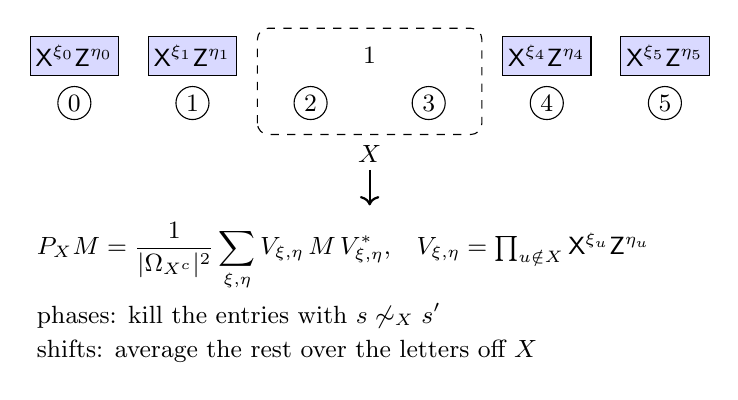
\begin{tikzpicture}[x=1.5cm,y=1cm,
  site/.style={circle,draw,fill=white,inner sep=1.6pt,font=\small},
  wbox/.style={draw,rectangle,inner sep=2pt,minimum height=0.5cm,font=\small,fill=Blue!15},
  region/.style={rounded corners=4pt,draw,dashed,fill=none},
  lab/.style={font=\small}]
  \foreach \u in {0,1,4,5} { \node[wbox] at (\u,0.6) {$\shift^{\xi_\u}\clock^{\eta_\u}$}; }
  \foreach \u in {0,...,5} { \node[site] at (\u,0) {\u}; }
  \draw[region] (1.55,-0.4) rectangle (3.45,0.95);
  \node[lab] at (2.5,-0.65) {$X$};
  \node[lab] at (2.5,0.6) {$1$};
  \draw[->,thick] (2.5,-0.85) -- (2.5,-1.3);
  \node[lab,anchor=west] at (-0.4,-1.95) {$P_XM=\dfrac1{|\Omega_{X^c}|^2}\displaystyle\sum_{\xi,\eta}
    V_{\xi,\eta}\,M\,V_{\xi,\eta}^*$,\quad $V_{\xi,\eta}=\prod_{u\notin X}\shift^{\xi_u}\clock^{\eta_u}$};
  \node[lab,anchor=west] at (-0.4,-2.7) {phases: kill the entries with $s\not\sim_Xs'$};
  \node[lab,anchor=west] at (-0.4,-3.15) {shifts: average the rest over the letters off $X$};
\end{tikzpicture}

\caption{\vet{The twirl onto $X=\{2,3\}$ on a chain of six sites. Each site off $X$ carries a
shift power and a clock power, with the letters $\xi_u$, $\eta_u$ of that site; the sites of $X$
carry the identity. Averaging $V_{\xi,\eta}MV_{\xi,\eta}^*$ over all letters off $X$ gives the
conditional expectation \eqref{eq:condexp}: the clock phases cancel every entry between
configurations that differ off $X$, and the shifts average the remaining entries over the
letters off $X$ (Theorem~\ref{thm:twirl}).}}
\label{fig:twirl}
\end{figure}

\begin{definition}[Weyl unitaries, twirl]\label{def:weyl}
\vet{For a region $Y$ and letters $\xi,\eta\in\Omega_Y$, the \emph{Weyl unitary} $V_{\xi,\eta}$ is
the matrix
\begin{equation}\label{eq:weyl}
  (V_{\xi,\eta})_{ss'}:=\ind{s=s'+\xi}\;\psi_\eta(s'),\qquad
  \psi_\eta(s):=\prod_{u\in Y}e_{q_u}\bigl(\eta(u)\,s(u)\bigr),
\end{equation}
the shift by $\xi$ applied after the clock phases $\psi_\eta$. The \emph{twirl} onto $X$ is the
average over the Weyl unitaries of the complement $Y=X^c$,
\begin{equation}\label{eq:twirl}
  \frac1{|\Omega_{Y}|^2}\sum_{\xi\in\Omega_Y}\sum_{\eta\in\Omega_Y}V_{\xi,\eta}\,M\,V_{\xi,\eta}^* .
\end{equation}}
\end{definition}

\begin{proposition}[Weyl unitaries]\label{prop:weyl}
\vet{$V_{\xi,\eta}$ is local to $Y$ and unitary, and for every $M$ and configurations $s,s'$
\begin{equation}\label{eq:weylconj}
  (V_{\xi,\eta}MV_{\xi,\eta}^*)_{ss'}=\psi_\eta(s-s')\;M_{s-\xi,\,s'-\xi} .
\end{equation}}
\end{proposition}

\begin{proof}
\vet{The phase $\psi_\eta(s)$ depends on $s|_Y$ only and is multiplicative in $s$, with
$\overline{\psi_\eta(s)}=\psi_\eta(-s)$ and $|\psi_\eta|=1$. The entry \eqref{eq:weyl} vanishes
unless $s\sim_Ys'$, since $s'+\xi\sim_Ys'$, and depends on the restrictions to $Y$ alone; so
$V_{\xi,\eta}$ is local to $Y$. In $V^*V$ and $VV^*$ the sums over the middle configuration
have one term, at $s+\xi$ and at $s-\xi$ respectively, where the phase meets its conjugate; both
products are the identity. In $(VMV^*)_{ss'}=\sum_{r,r'}V_{sr}M_{rr'}\overline{V_{s'r'}}$ the
only term is $r=s-\xi$, $r'=s'-\xi$, with the phase
$\psi_\eta(s-\xi)\overline{\psi_\eta(s'-\xi)}=\psi_\eta(s-s')$, the $\xi$ cancelling.}
\end{proof}

\needspace{10\baselineskip}
\begin{theorem}[the twirl is the conditional expectation]\label{thm:twirl}
\vet{For cyclic alphabets the twirl \eqref{eq:twirl} onto $X$ equals $P_XM$ for every $M$.}
\end{theorem}

\begin{proof}
\vet{By \eqref{eq:weylconj} the entry of the twirl at $(s,s')$ is
\[
  \frac1{|\Omega_Y|^2}\sum_{\xi}M_{s-\xi,s'-\xi}\sum_{\eta}\psi_\eta(s-s'),\qquad\text{and}\qquad
  \sum_\eta\psi_\eta(s-s')=\prod_{u\in Y}\;\sum_{l\in\Z_{q_u}}e_{q_u}\bigl(l\,(s(u)-s'(u))\bigr)
\]
equals $|\Omega_Y|\,\ind{s\sim_Xs'}$ by \eqref{eq:charsum} at each site. For $s\sim_Xs'$ the letters of $s$ and $s'$ off $X$ agree,
so $s-\xi=(s|_X,\zeta)$ and $s'-\xi=(s'|_X,\zeta)$ with $\zeta:=s|_Y-\xi$, and as $\xi$ runs over
$\Omega_Y$ so does $\zeta$. The remaining sum is that of \eqref{eq:condexp}, with the
normalization $|\Omega_Y|/|\Omega_Y|^2=1/|\Omega_Y|$.}
\end{proof}

\needspace{10\baselineskip}
\begin{proposition}[contraction and bimodule property]\label{prop:bimodule}
\vet{For cyclic alphabets, $\norm{P_XM}\le\norm M$, and $P_X(aMb)=a\,(P_XM)\,b$ for
$a,b\in\cA(X)$.}
\end{proposition}

\begin{proof}
\vet{Each term $V_{\xi,\eta}MV_{\xi,\eta}^*$ of the twirl has the norm of $M$, and the norm of an
average is at most the average of the norms. For $a,b\in\cA(X)$ and $V$ local to $X^c$,
$V(aMb)V^*=a(VMV^*)b$ by causality (Theorem~\ref{thm:quditnet}), termwise in the average.}
\end{proof}

\begin{theorem}[local approximation]\label{thm:localapprox}
\vet{For cyclic alphabets, every $M\in\Mat_\Lambda$ and every region $X$,
\begin{equation}\label{eq:localapproxqudit}
  \norm{M-P_XM}\le N_{X^c}(M)\le2\,\norm{M-P_XM}.
\end{equation}
The qudit net with cyclic alphabets has local approximation with $P_X$.}
\end{theorem}

\begin{proof}
\vet{Since $VV^*=1$, $M-VMV^*=\comm MV\,V^*$ for each Weyl unitary $V$ of the complement, so
$M-P_XM$ is the average of the $\comm MV\,V^*$. Each has norm at most
$\norm{\comm MV}\le N_{X^c}(M)$, because $V\in\cA(X^c)$ has norm one; so does the average. The
second inequality is Proposition~\ref{prop:converse}(a) with \vetnew{$c=M$ and
$c'=P_XM\in\cA(X)$}.}
\end{proof}

\vet{The constant $2$ is attained: for a single qubit outside $X$ and $M=\sigma^x$ at that site,
$P_XM=0$, $\norm{M-P_XM}=1$, and $N_{X^c}(M)=2$ (at least $\norm{\comm{\sigma^x}{\sigma^z}}=2$,
at most $2\norm M$). The constant $1$ is approached along the following family:
for $X=\emptyset$, \vetnew{one site with an alphabet of $n\ge2$ letters} and $M$ a rank-one
projection $|e\rangle\langle e|$, \vetnew{$\norm{M-P_\emptyset M}=1-1/n$} while $N_\Lambda(M)=1$ (the commutator of a projection with an
element of norm at most one has two off-diagonal blocks of norm at most one, and
$|e\rangle\langle f|+|f\rangle\langle e|$ with $f\perp e$ gives one).}

\subsection{Truncated dynamics and the approximate automaton}

\vet{Let $(S_i,L_i,\kappa_i)_{i\in I}$ be a family of local generators on a causal net with local
approximation, $A(t)=e^{tL}a$ for $a\in\cA(X)$, and let $X'\supseteq X$ be a larger region. The
walk bound of Chapter~\ref{sec:closed} controls the commutator of $A(t)$ with every observable
of $Y:=X'^c$; local approximation turns this into a distance.}

\needspace{14\baselineskip}
\begin{theorem}[truncated dynamics]\label{thm:truncated}
\vet{For $a\in\cA(X)$, $X\subseteq X'$, $Y=X'^c$ and $t\ge0$, with \vetnew{the walk terms $\omega_k(t)$ of Chapter~\ref{sec:closed} for the pair $(Y,X)$,
eq.~\eqref{eq:walkterms}},
\begin{equation}\label{eq:truncated}
  \norm{A(t)-P_{X'}A(t)}\le N_Y(A(t))\le2\norm a\sum_{k\ge0}\omega_k(t).
\end{equation}
Under bounded geometry $(g,\ell,p,\rho)$ with distance $d$ and $v=2g\ell p$, if
$(r-1)\rho<d(y,x)$ for all $y\in\bd Y$ and $x\in X\cap T$ (an integer $r\ge1$), the right side is
at most
$2\norm a\,|\bd Y|\,(vt)^re^{vt}/r!$ and, for every real $\mu$, at most
$2\norm a\,|\bd Y|\,e^{vt}e^{-\mu r}(e^{e^\mu vt}-1)$.}
\end{theorem}

\begin{proof}
\vet{The first inequality is local approximation. For the second, $N_Y(A(t))$ is the supremum
of $\norm{\comm{A(t)}b}$ over $b\in\cA(Y)$ with $\norm b\le1$, and the walk bound
(Theorem~\ref{thm:walkseries}) gives $2\norm a\norm b\,(\ind{X\cap Y\ne\emptyset}+\sum_k\omega_k(t))$
with $X\cap Y=\emptyset$. The geometric forms are those of Chapter~\ref{sec:closed} for the
walk series.}
\end{proof}

\vet{So $P_{X'}A(t)$ is an observable of $X'$ within a light-cone tail of $A(t)$. Read as a
property of the map $e^{tL}$, this is approximate locality with a neighbourhood map. The
natural map is the $r$-neighbourhood $O^{+r}:=\{w:\,d(w,x)<r\rho\text{ for some }x\in O\}$,
measured from the site into the region (the distance need not be symmetric).}

\needspace{10\baselineskip}
\begin{corollary}[approximate automaton]\label{cor:automaton}
\vet{\begin{enumerate}[label=(\alph*),nosep]
\item For $\Lambda$ finite and a neighbourhood map $\mathcal N$ with $O\subseteq\mathcal N(O)$
  for all $O$, $e^{tL}$ is $\varepsilon(t)$-local with $\mathcal N$, where $\varepsilon(t)$ is
  the largest, over the finitely many regions $O$, of the errors $2\sum_k\omega_k(t)$ of the
  pairs $(\mathcal N(O)^c,O)$.
\item Under bounded geometry with $\rho>0$ and an integer $r\ge1$, $e^{tL}$ is
  \vetnew{$\varepsilon_r(t)$-local with $O\mapsto O^{+r}$, where $\varepsilon_r(t)$ is either of}
  \begin{align}
    \varepsilon_r(t)&=2|T|\,\frac{(vt)^r}{r!}e^{vt},\label{eq:epsr}\\
    \varepsilon_r(t)&=2|T|\,e^{vt}e^{-\mu r}\bigl(e^{e^\mu vt}-1\bigr)\qquad(\mu\in\R).\label{eq:epsrcone}
  \end{align}
\end{enumerate}}
\end{corollary}

\begin{proof}
\vet{\begin{enumerate}[label=(\alph*),nosep]
\item For $c\in\cA(O)$ take $P_{\mathcal N(O)}e^{tL}c$ as the nearby element of
  Definition~\ref{def:localapprox} and apply \eqref{eq:truncated} with $X=O$,
  $X'=\mathcal N(O)$; the maximum over $O$ makes the error uniform.
\item $O\subseteq O^{+r}$ since $d(u,u)=0<r\rho$. A site $w\notin O^{+r}$ has $d(w,u)\ge r\rho
  >(r-1)\rho$ for every $u\in O$, so the geometric form applies, and $|\bd Y|\le|T|$ because the
  boundary consists of touched sites.\qedhere
\end{enumerate}}
\end{proof}

\vetnew{At fixed $t$ the first error of (b) vanishes as $r\to\infty$, since $(vt)^r/r!\to0$, and
the second, for $\mu>0$, is at most $2|T|\,e^{(1+e^\mu)vt-\mu r}$, so exponentially small in $r$
once $r>(1+e^\mu)vt/\mu$: up to time $t$ the dynamics is a cellular automaton with the
neighbourhood $O^{+r}$, $r$ of order $vt$, up to an exponentially small error.}

\begin{example}[truncation on a chain]\label{ex:truncation}
\vet{On a chain of five qubits with $H=\sum_{u=0}^{3}\bigl(\sigma^z_u\sigma^z_{u+1}
+\tfrac12\sigma^x_u\sigma^x_{u+1}\bigr)$ and $a=\sigma^x_0$, the error
$\norm{A(t)-P_{X_r}A(t)}$ for $X_r=\{0,\dots,r\}$ against the walk bound \eqref{eq:truncated}:
at $t=0.3$ the error is $0.56$, $0.086$, $0.017$ for $r=0,1,2$, against the bounds $9.6$, $4.6$,
$1.4$; at $t=0.1$ and $r=2$ the error is $6.6\cdot10^{-4}$ against $1.6\cdot10^{-2}$. The error
decays with $r$ as the bound predicts; the bound overshoots by factors between $17$ and $82$ at
these times, and the first two bounds quoted exceed the trivial bound $2\norm a$. For
$X_r=\Lambda$ the error is zero, as $A(t)$ is then local to $X_r$.}

\vetnew{On twelve qubits with the same Hamiltonian and observable the light cone is visible
(Figure~\ref{fig:longchain}). At $t=0.25$, $0.5$, $1$, $2$ the error falls below $0.1$ from
$r=1$, $2$, $4$, $7$ on: a front moving at about $3.5$ sites per unit time. Beyond the front the
error decays by a constant factor per site, as $e^{-3.07r}$, $e^{-2.38r}$, $e^{-1.66r}$,
$e^{-0.86r}$ at the four times (least squares over $r=3,\dots,10$), the rate falling as the
front approaches.

The walk bound \eqref{eq:truncated} decays in $r$ in the same way, at the
smaller rates $e^{-2.34r}$, $e^{-1.67r}$, $e^{-1.05r}$, $e^{-0.57r}$; it is below the trivial
bound $2\norm a$ from $r=2$ on at $t=0.25$ and from $r=5$ on at $t=0.5$, and trivial for every
$r\le10$ at $t=1$ and $t=2$, where its velocity has outrun the chain. It exceeds the error by
factors from $12$ to above $10^{10}$. The bounded-geometry bound with $v=16$ is trivial
throughout. Corollary~\ref{cor:automaton} and the paragraph after it predict the exponential
decay in the radius and a front moving linearly in $t$; the velocity they give exceeds the
observed one.}
\end{example}

\begin{figure}[htb]
\centering
% Figure: the twelve-qubit truncation errors of Example ex:truncation, generated by
% checks/long_chain_figure.py from the data of checks/long_chain.py. Transcription (for
% cheap agents): axes, the radius r = 0..10 of the region X_r to the right and the error
% eps_r(t) upward on a logarithmic scale from 1e-12 to 10; one solid curve with dots per
% time t = 0.25, 0.5, 1, 2 (labelled at its right end), each falling exponentially in r
% beyond a front that moves to the right with t; the walk bound dashed, for t = 0.25 and
% 0.5 only, where it is below the trivial bound 2 (a thin horizontal line at 2).
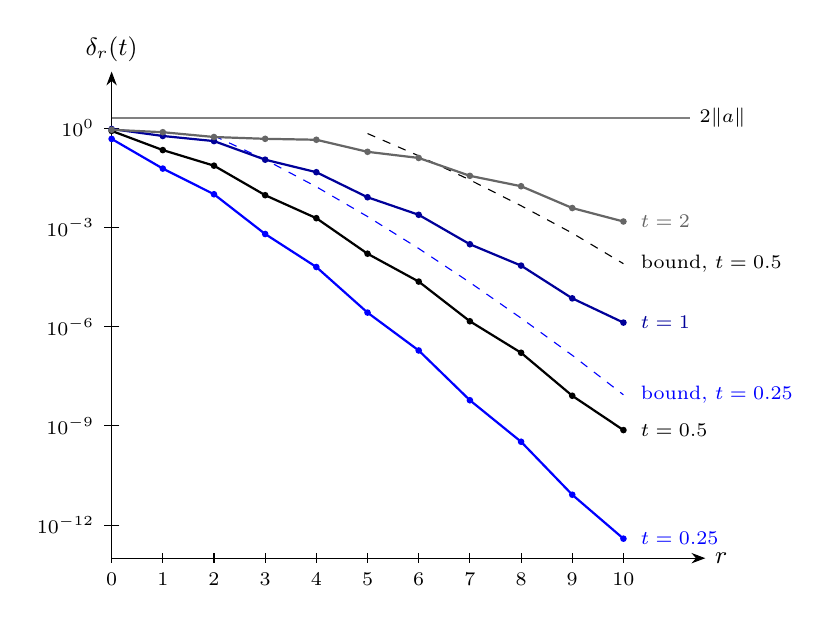
\begin{tikzpicture}[x=0.65cm,y=1cm,>={Stealth[length=5pt]}]
  \draw[->] (0,0) -- (11.6,0) node[right,font=\small] {$r$};
  \draw[->] (0,0) -- (0,6.18) node[above,font=\small] {$\delta_r(t)$};
  \draw (0.15,0.42) -- (-0.15,0.42) node[left,font=\scriptsize] {$10^{-12}$};
  \draw (0.15,1.68) -- (-0.15,1.68) node[left,font=\scriptsize] {$10^{-9}$};
  \draw (0.15,2.94) -- (-0.15,2.94) node[left,font=\scriptsize] {$10^{-6}$};
  \draw (0.15,4.20) -- (-0.15,4.20) node[left,font=\scriptsize] {$10^{-3}$};
  \draw (0.15,5.46) -- (-0.15,5.46) node[left,font=\scriptsize] {$10^{0}$};
  \draw (0,0.06) -- (0,-0.06) node[below,font=\scriptsize] {0};
  \draw (1,0.06) -- (1,-0.06) node[below,font=\scriptsize] {1};
  \draw (2,0.06) -- (2,-0.06) node[below,font=\scriptsize] {2};
  \draw (3,0.06) -- (3,-0.06) node[below,font=\scriptsize] {3};
  \draw (4,0.06) -- (4,-0.06) node[below,font=\scriptsize] {4};
  \draw (5,0.06) -- (5,-0.06) node[below,font=\scriptsize] {5};
  \draw (6,0.06) -- (6,-0.06) node[below,font=\scriptsize] {6};
  \draw (7,0.06) -- (7,-0.06) node[below,font=\scriptsize] {7};
  \draw (8,0.06) -- (8,-0.06) node[below,font=\scriptsize] {8};
  \draw (9,0.06) -- (9,-0.06) node[below,font=\scriptsize] {9};
  \draw (10,0.06) -- (10,-0.06) node[below,font=\scriptsize] {10};
  \draw[thin,black!50] (0,5.59) -- (11.3,5.59) node[right,font=\scriptsize,black] {$2\norm a$};
  \draw[Blue,thick] (0,5.325) -- (1,4.948) -- (2,4.622) -- (3,4.117) -- (4,3.698) -- (5,3.119) -- (6,2.638) -- (7,2.006) -- (8,1.479) -- (9,0.806) -- (10,0.248);
  \fill[Blue] (0,5.325) circle (1.2pt);
  \fill[Blue] (1,4.948) circle (1.2pt);
  \fill[Blue] (2,4.622) circle (1.2pt);
  \fill[Blue] (3,4.117) circle (1.2pt);
  \fill[Blue] (4,3.698) circle (1.2pt);
  \fill[Blue] (5,3.119) circle (1.2pt);
  \fill[Blue] (6,2.638) circle (1.2pt);
  \fill[Blue] (7,2.006) circle (1.2pt);
  \fill[Blue] (8,1.479) circle (1.2pt);
  \fill[Blue] (9,0.806) circle (1.2pt);
  \fill[Blue] (10,0.248) circle (1.2pt);
  \node[Blue,anchor=west,font=\scriptsize] at (10.15,0.248) {$t=0.25$};
  \draw[Blue,dashed] (2,5.364) -- (3,5.062) -- (4,4.717) -- (5,4.339) -- (6,3.933) -- (7,3.502) -- (8,3.049) -- (9,2.577) -- (10,2.075);
  \node[Blue,anchor=west,font=\scriptsize] at (10.15,2.075) {bound, $t=0.25$};
  \draw[black,thick] (0,5.427) -- (1,5.183) -- (2,4.985) -- (3,4.610) -- (4,4.318) -- (5,3.867) -- (6,3.513) -- (7,3.009) -- (8,2.609) -- (9,2.063) -- (10,1.627);
  \fill[black] (0,5.427) circle (1.2pt);
  \fill[black] (1,5.183) circle (1.2pt);
  \fill[black] (2,4.985) circle (1.2pt);
  \fill[black] (3,4.610) circle (1.2pt);
  \fill[black] (4,4.318) circle (1.2pt);
  \fill[black] (5,3.867) circle (1.2pt);
  \fill[black] (6,3.513) circle (1.2pt);
  \fill[black] (7,3.009) circle (1.2pt);
  \fill[black] (8,2.609) circle (1.2pt);
  \fill[black] (9,2.063) circle (1.2pt);
  \fill[black] (10,1.627) circle (1.2pt);
  \node[black,anchor=west,font=\scriptsize] at (10.15,1.627) {$t=0.5$};
  \draw[black,dashed] (5,5.393) -- (6,5.110) -- (7,4.804) -- (8,4.476) -- (9,4.129) -- (10,3.740);
  \node[black,anchor=west,font=\scriptsize] at (10.15,3.740) {bound, $t=0.5$};
  \draw[Blue!60!black,thick] (0,5.451) -- (1,5.362) -- (2,5.297) -- (3,5.061) -- (4,4.902) -- (5,4.584) -- (6,4.361) -- (7,3.987) -- (8,3.716) -- (9,3.300) -- (10,2.992);
  \fill[Blue!60!black] (0,5.451) circle (1.2pt);
  \fill[Blue!60!black] (1,5.362) circle (1.2pt);
  \fill[Blue!60!black] (2,5.297) circle (1.2pt);
  \fill[Blue!60!black] (3,5.061) circle (1.2pt);
  \fill[Blue!60!black] (4,4.902) circle (1.2pt);
  \fill[Blue!60!black] (5,4.584) circle (1.2pt);
  \fill[Blue!60!black] (6,4.361) circle (1.2pt);
  \fill[Blue!60!black] (7,3.987) circle (1.2pt);
  \fill[Blue!60!black] (8,3.716) circle (1.2pt);
  \fill[Blue!60!black] (9,3.300) circle (1.2pt);
  \fill[Blue!60!black] (10,2.992) circle (1.2pt);
  \node[Blue!60!black,anchor=west,font=\scriptsize] at (10.15,2.992) {$t=1$};
  \draw[black!60,thick] (0,5.441) -- (1,5.410) -- (2,5.349) -- (3,5.326) -- (4,5.314) -- (5,5.161) -- (6,5.083) -- (7,4.856) -- (8,4.724) -- (9,4.447) -- (10,4.276);
  \fill[black!60] (0,5.441) circle (1.2pt);
  \fill[black!60] (1,5.410) circle (1.2pt);
  \fill[black!60] (2,5.349) circle (1.2pt);
  \fill[black!60] (3,5.326) circle (1.2pt);
  \fill[black!60] (4,5.314) circle (1.2pt);
  \fill[black!60] (5,5.161) circle (1.2pt);
  \fill[black!60] (6,5.083) circle (1.2pt);
  \fill[black!60] (7,4.856) circle (1.2pt);
  \fill[black!60] (8,4.724) circle (1.2pt);
  \fill[black!60] (9,4.447) circle (1.2pt);
  \fill[black!60] (10,4.276) circle (1.2pt);
  \node[black!60,anchor=west,font=\scriptsize] at (10.15,4.276) {$t=2$};
\end{tikzpicture}

\caption{\vetnew{The truncation error $\delta_r(t)=\norm{A(t)-P_{X_r}A(t)}$ on a chain of
twelve qubits, $H=\sum_u(\sigma^z_u\sigma^z_{u+1}+\tfrac12\sigma^x_u\sigma^x_{u+1})$,
$a=\sigma^x_0$, $X_r=\{0,\dots,r\}$, against $r$ on a logarithmic scale, one curve per time
$t$. Dashed: the walk bound \eqref{eq:truncated} where it is below the trivial bound $2\norm a$
(at $t=1$ and $2$ it is trivial for every $r$ shown). Beyond a front that moves with $t$ the
error decays exponentially in $r$; the bound shares the decay, with a smaller rate and a far
larger prefactor.}}
\label{fig:longchain}
\end{figure}

\subsection{Open systems}

\vet{A quantum system in contact with an environment evolves, after the environment has been
traced out and under the Markov approximation, by a semigroup $e^{tL}$ of unital completely
positive maps, whose generator has the Lindblad form. In the Heisenberg picture, for a
Hamiltonian $H$ and \vetnew{finitely many} \emph{jump operators} \vetnew{$\Gamma_j$},
\begin{equation}\label{eq:lindblad}
  La=\ii\comm Ha+\vetnew{\sum_j}\Bigl(\Gamma_j^*a\Gamma_j-\tfrac12\bigl(\Gamma_j^*\Gamma_ja
  +a\Gamma_j^*\Gamma_j\bigr)\Bigr).
\end{equation}
The jump terms describe the environment's action: a measurement-like kick $a\mapsto\Gamma^*a\Gamma$
balanced by the anticommutator that keeps $L1=0$. On a lattice the Hamiltonian and the jumps
are local, and the generator is a sum of local terms.}

\needspace{8\baselineskip}
\begin{definition}[Lindblad terms and families]\label{def:lindbladterm}
\vet{A \emph{Lindblad term} on a finite region $S$ is a self-adjoint $H\in\cA(S)$ with \vetnew{finitely many jump
operators $\Gamma_j\in\cA(S)$}; its generator $L_S$ is \eqref{eq:lindblad}, and
the \emph{dissipator} of one jump is
$\Delta_\Gamma a:=\Gamma^*a\Gamma-\tfrac12(\Gamma^*\Gamma a+a\Gamma^*\Gamma)$, so that
$L_S=\ad_H+\sum_j\Delta_{\Gamma_j}$ \vetnew{(with no jumps the term is a Hamiltonian one)}. A
\emph{Lindblad family} is a finite family $(S_i,L_i)_{i\in I}$ of Lindblad terms, with
Hamiltonian parts $H_i$ and \vetnew{jumps $\Gamma_{ij}$, finitely many $j$ for each $i$}, together with the hypothesis
that every sub-family is \emph{contractive}: $\norm{e^{tL_J}}\le1$ for all $J\subseteq I$ and
$t\ge0$.}
\end{definition}

\vet{The contraction hypothesis is physics: $e^{tL_J}$ is unital and completely positive, and
a unital positive map between C*-algebras has norm one. Neither that norm theorem nor the
product formula that passes from the terms to their sum is reproved here; the hypothesis is
carried explicitly, and one case, a single dephasing jump, is proved below
(Proposition~\ref{prop:dephasing}).}

\needspace{10\baselineskip}
\begin{proposition}[Lindblad terms]\label{prop:lindbladterm}
\vet{For a Lindblad term on $S$ and a causal net:
\begin{enumerate}[label=(\alph*),nosep]
\item $L_S$ is bounded, $\norm{L_S}\le2\norm H+2\sum_j\norm{\Gamma_j}^2$;
\item $L_Sc=0$ for $c\in\cA(S^c)$;
\item $L_Sc\in\cA(Z\cup S)$ for $c\in\cA(Z)$ (support closure, G2);
\item $(L_Sa)^*=L_S(a^*)$.
\end{enumerate}}
\end{proposition}

\begin{proof}
\vet{\begin{enumerate}[label=(\alph*),nosep]
\item $\norm{\ad_Ha}\le2\norm H\norm a$ by \eqref{eq:ad}; the three maps
  $a\mapsto\Gamma^*a\Gamma$, $\tfrac12\Gamma^*\Gamma a$, $\tfrac12a\Gamma^*\Gamma$ have norms at most
  $\norm\Gamma^2$, $\tfrac12\norm\Gamma^2$, $\tfrac12\norm\Gamma^2$.
\item $c$ commutes with $H$, $\Gamma_j$ and $\Gamma_j^*$ by causality ($\cA(S)$ is closed under
  adjoints), so $\comm Hc=0$ and
  $\Gamma_j^*c\Gamma_j=\Gamma_j^*\Gamma_jc=\tfrac12(\Gamma_j^*\Gamma_jc+c\Gamma_j^*\Gamma_j)$.
\item Every factor lies in $\cA(Z\cup S)$ by isotony, which is closed under products and sums.
\item $(\ii\comm Ha)^*=\ii\comm H{a^*}$ for self-adjoint $H$, $(\Gamma^*a\Gamma)^*=\Gamma^*a^*\Gamma$,
  and the two halves of the anticommutator exchange.\qedhere
\end{enumerate}}
\end{proof}

\begin{theorem}[locality in the argument for Lindblad terms]\label{thm:lindbladG1}
\vet{For a Lindblad term on $S$ and every $c$:
\begin{enumerate}[label=(\alph*),nosep]
\item on any net, $\norm{\Delta_\Gamma c}\le\norm\Gamma^2N_S(c)$ for $\Gamma\in\cA(S)$, hence
  \begin{equation}\label{eq:lindbladG1direct}
    \norm{L_Sc}\le\bigl(\norm H+\textstyle\sum_j\norm{\Gamma_j}^2\bigr)N_S(c);
  \end{equation}
\item on a causal net with local approximation, $L_Sc=L_S(c-P_{S^c}c)$ and
  \begin{equation}\label{eq:lindbladG1}
    \norm{L_Sc}\le\norm{L_S}\,N_S(c)\le\bigl(2\norm H+2\textstyle\sum_j\norm{\Gamma_j}^2\bigr)N_S(c).
  \end{equation}
\end{enumerate}}
\end{theorem}

\begin{proof}
\vet{\begin{enumerate}[label=(\alph*),nosep]
\item The dissipator is a sum of two commutators,
  $\Delta_\Gamma c=\tfrac12\Gamma^*\comm c\Gamma+\tfrac12\comm{\Gamma^*}c\,\Gamma$ (expand both
  sides), and $\norm{\comm cx}\le\norm x\,N_S(c)$ for $x\in\cA(S)$
  (Proposition~\ref{prop:derivation}), applied to $x=\Gamma$ and $x=\Gamma^*$; the Hamiltonian
  part is Proposition~\ref{prop:derivation} again.
\item $P_{S^c}c\in\cA(S^c)$, so $L_S(P_{S^c}c)=0$ by Proposition~\ref{prop:lindbladterm}(b) and
  $L_Sc=L_S(c-P_{S^c}c)$ by linearity. Then
  $\norm{L_Sc}\le\norm{L_S}\norm{c-P_{S^c}c}\le\norm{L_S}N_S(c)$ by \eqref{eq:localapprox} for
  the region $S^c$, whose complement is $S$.\qedhere
\end{enumerate}}
\end{proof}

\vet{Route (a) is the sharper one: it needs neither causality nor the conditional expectation,
and with no jumps it returns the Hamiltonian strength $\norm H$ of Chapter~\ref{sec:qudit}.
Route (b) is the mechanism in one line: a term acts only on what an observable does inside its
support, the conditional expectation isolates that part, and the strength is the norm of the
term, the form in which the literature states the open-system bound.}

\needspace{14\baselineskip}
\begin{theorem}[open systems as local generators]\label{thm:opensystems}
\vet{On a causal net, a Lindblad family $(S_i,L_i)_{i\in I}$ is a family of local generators
with the strengths $\kappa_i=\norm{H_i}+\sum_j\norm{\Gamma_{ij}}^2$; with local approximation
also with $\kappa_i=\norm{L_i}$, and with $\kappa_i=2\norm{H_i}+2\sum_j\norm{\Gamma_{ij}}^2$.
Consequently the path-sum bound and its closed forms for $t\ge0$
(Chapters~\ref{sec:master}--\ref{sec:closed}\vetnew{)} hold for $A(t)=e^{tL}a$: for $a\in\cA(X)$, $b\in\cA(Y)$,
\[
  \norm{\comm{A(t)}b}\le2\norm a\norm b\Bigl(\ind{X\cap Y\ne\emptyset}+\sum_{k\ge0}\omega_k(t)\Bigr),
\]
\vetnew{where the walk terms $\omega_k(t)$ of \eqref{eq:walkterms} carry the strengths used: the
direct strengths $\norm{H_i}+\sum_j\norm{\Gamma_{ij}}^2$, or, under local approximation,
$\norm{L_i}$ or its bound $2\norm{H_i}+2\sum_j\norm{\Gamma_{ij}}^2$;} the light cone under
bounded geometry, and the truncated dynamics of
Theorem~\ref{thm:truncated}.}
\end{theorem}

\begin{proof}
\vet{G1 is Theorem~\ref{thm:lindbladG1}, (a) or (b), G2 is Proposition~\ref{prop:lindbladterm}(c),
G3 is the contraction hypothesis; the largest strengths dominate $\norm{L_i}$, and G1 is
monotone in $\kappa$.}
\end{proof}

\vetnew{The bounds are for $t\ge0$. In general a Lindblad family has no contractive negation, and
the time-reversed forms of Theorem~\ref{thm:reverse} are not available: for the dephasing term of
Proposition~\ref{prop:dephasing} below and an $a$ with $\Gamma a\Gamma=-a$ (such as $\sigma^x$ for
$\Gamma=\sigma^z$), \eqref{eq:dephasing} at the time $-t<0$ gives $e^{-t\Delta_\Gamma}a=e^{2t}a$,
of norm larger than $\norm a$. A family without jumps is a Hamiltonian family, whose negation is
contractive (Theorem~\ref{thm:hamgenerators}).}

\needspace{10\baselineskip}
\begin{proposition}[a dephasing term is contractive]\label{prop:dephasing}
\vet{For a self-adjoint jump $\Gamma$ with $\Gamma^2=1$ and no Hamiltonian part,
$\Delta_\Gamma a=\Gamma a\Gamma-a$, $\Delta_\Gamma^2=-2\Delta_\Gamma$, and for every real $t$
\begin{equation}\label{eq:dephasing}
  e^{t\Delta_\Gamma}a=\tfrac{1+e^{-2t}}2\,a+\tfrac{1-e^{-2t}}2\,\Gamma a\Gamma ;
\end{equation}
for $t\ge0$ this is a convex combination of $a$ and a unitary conjugate, so
$\norm{e^{t\Delta_\Gamma}}\le1$.}
\end{proposition}

\begin{proof}
\vet{Such a $\Gamma$ is a two-valued observable, and the term is pure dephasing in its eigenbasis.
With $\Gamma^*\Gamma=1$ the dissipator is $\Theta-\mathrm{id}$ for $\Theta:a\mapsto\Gamma a\Gamma$,
and $\Theta^2=\mathrm{id}$, so $\Delta_\Gamma^{n+1}=(-2)^n\Delta_\Gamma$. Summing the exponential
series, $e^{t\Delta_\Gamma}=\mathrm{id}+\sum_{n\ge0}\frac{t^{n+1}(-2)^n}{(n+1)!}\Delta_\Gamma
=\mathrm{id}+\frac{1-e^{-2t}}2\Delta_\Gamma$, which is \eqref{eq:dephasing}. Both $\mathrm{id}$
and $\Theta$ have norm at most one ($\Gamma$ is unitary), and the coefficients are nonnegative
for $t\ge0$.}
\end{proof}

\begin{example}[two qubits with dephasing]\label{ex:dephasing}
\vet{Two qubits, $H=\sigma^x_0\sigma^x_1$, one jump $\Gamma=\sigma^z_0$, and the observables
$a=\sigma^z_0$, $b=\sigma^z_1$ of Example~\ref{ex:twoqubit}. The dissipator vanishes on $a$,
since $a$ commutes with $\Gamma$, so $La=\ii\comm Ha$ and the derivative of $\comm{A(t)}b$ at
$t=0$ is the nonzero double commutator of Chapter~\ref{sec:qudit}; hence $\comm{A(t)}b\ne0$ for
some $t>0$ (the contraction of this term, whose Hamiltonian part does not commute with the jump,
is the carried hypothesis, not Proposition~\ref{prop:dephasing}).}
\end{example}

\vetnew{For a three-qubit family with
random Hamiltonian and jump terms on $\{0,1\}$ and $\{1,2\}$ and $a=\sigma^x_0$,
$\norm{\comm{A(t)}{\sigma^x_2}}$ is $0$ at $t=0$ and $0.11$ at $t=0.5$; for the same $a$ and
$b=\sigma^z_2$ at $t=0.3$ the commutator norm is $0.026$ against the walk bound $4.5$ with the
strengths $\norm{L_i}$ and $272$ with the strengths $2\norm{H_i}+2\sum_j\norm{\Gamma_{ij}}^2$.
Both bounds exceed the trivial bound $2$; the first overshoots by a factor of $170$, more than
the Hamiltonian bounds above, and the larger strengths cost a further factor of $60$ (the
direct strengths of Theorem~\ref{thm:lindbladG1}(a) are half of them, and the series they enter
is correspondingly smaller).}

\subsection*{Notes and references}
\vetnew{\emph{Local approximation.} The review \cite{chen-lucas-yin}, its Proposition~4.1, states
for the expectation $\mathbb E_S$ onto a region $S$, the Haar average over the unitaries of the
complement of $S$,
\[
  \norm{\mathbb E_SA-A}\le\sup_B\norm{\comm AB}\le2\norm{\mathbb E_SA-A},
\]
the supremum over the unit operators $B$ on the complement. Theorem~\ref{thm:localapprox} is
this statement with $S=X$, $A=M$ and $\mathbb E_S=P_X$: the Haar average and the finite twirl
over the Weyl unitaries are both the normalized partial trace over the complement, re-embedded
(Theorem~\ref{thm:twirl}), and the supremum is $N_{X^c}(M)$.

\emph{Truncated dynamics.} The review's Proposition~4.3
bounds the distance from $\tau_t(A)$ to the evolution under the Hamiltonian restricted to a
larger region; Theorem~\ref{thm:truncated} matches it in shape, an observable of the larger
region within the tail of the walk series, with the conditional expectation $P_{X'}A(t)$ as the
local approximant and the constants of these notes.

\emph{Open systems.} The review's Theorem~3.14 is its Lieb-Robinson bound for a local Lindblad
generator, for $t\ge0$, with the norms of the Lindblad terms as strengths. On the qudit net with
cyclic alphabets, which has local approximation (Theorem~\ref{thm:localapprox}),
Theorem~\ref{thm:opensystems} with $\kappa_i=\norm{L_i}$ and Proposition~\ref{prop:finite} give
it in the notation of the review's (3.36) recalled at the end of Chapter~\ref{sec:qudit}:
\[
  \mathcal C_{AB}(t)\le\sum_{u\in A,\,v\in B}\bigl(e^{2th}\bigr)_{uv}\quad(t\ge0),\qquad
  h_{uv}=\sum_{i:\,u,v\in S_i}\norm{L_i},
\]
by the argument given there. The review obtains the contraction of the sub-families from
complete positivity; here it is the hypothesis carried in Definition~\ref{def:lindbladterm}.}

\paragraph{Checks.} {\small The twirl against the partial trace (exactly for qubits, numerically
for qutrits), the properties of the conditional expectation, the estimate
\eqref{eq:localapproxqudit} with the attained factor $2$, the truncation errors on chains of
three and five qubits \vetnew{(section~3 of the script; the chapter quotes the five-site
numbers)}, the contractivity, the vanishing off the support, the mechanism
$L_Sc=L_S(c-P_{S^c}c)$, the strengths and the walk bound for the random Lindblad family\vetnew{ (section~4 of the script)}, and the
degenerate cases ($X=\Lambda$, $X=\emptyset$, no jumps, $t=0$) are computed by
\texttt{checks/m3\_check.py}. \vetnew{The twelve-qubit errors and bounds of
Example~\ref{ex:truncation} are computed by \texttt{checks/long\_chain.py}; the fronts, decay rates, ratios and Figure~\ref{fig:longchain} by
\texttt{checks/long\_chain\_figure.py}.}}


\section{Fermions}\label{sec:fermions}
\vetnew{This chapter is to come.}

\FloatBarrier
\section{Harmonic oscillators}\label{sec:harmonic}

\motiv{\vetnew{The bounds so far are for bounded local generators: spins and open systems. Harmonic
lattice bosons have an unbounded Hamiltonian and an infinite-dimensional algebra, so the generator
of their dynamics has no finite strength and the path-sum bound of
Chapter~\ref{sec:master} does not apply to them. What replaces it is a
different mechanism, special to quadratic Hamiltonians: their dynamics moves the Weyl operators
along a linear flow of the classical phase space, $\alpha_t(W(f))=W(T_tf)$, and the Weyl relation
turns the commutator of two Weyl operators into a phase, so that the whole question reduces to
the entries of the classical propagator $T_t=e^{tK}$.

We bound these entries by the
exponential of the entrywise absolute value $\abs K$, a nonnegative matrix in the role
of the site matrix of Chapter~\ref{sec:closed}: the range form $(vt)^r/r!\,e^{vt}$ and the light
cone come over unchanged, with the classical generator in place of the interaction.}}

\subsection{The lattice phase space and the Weyl operators}

\vetnew{Throughout, $\Lambda$ is a finite set of sites. The phase space is
$V=\Lambda\to\R^2$, a position coordinate $f^q_x$ and a momentum coordinate $f^p_x$ at every
site, equivalently a function on the coordinates $\Lambda'=\Lambda\times\{q,p\}$. For a
coordinate $a=(x,q)$ write $\bar a=(x,p)$ and conversely, and $\site(a)=x$. The symplectic form
is
\begin{equation}\label{eq:sigma}
\sigma(f,g)=\sum_{x\in\Lambda}\bigl(f^q_xg^p_x-f^p_xg^q_x\bigr)=f\cdot\Omega g,
\qquad \Omega_{(x,q),(x,p)}=1,\ \Omega_{(x,p),(x,q)}=-1,
\end{equation}
all other entries of $\Omega$ being zero; it is bilinear and alternating,
$\sigma(f,f)=0$. The support of $f$ is the set of sites where a coordinate of $f$ is nonzero, and
for $X\subseteq\Lambda$ we write $X'=X\times\{q,p\}$ and $\norm f_1=\sum_a\abs{f_a}$.}

\begin{definition}[Weyl system, CCR algebra]\label{def:weylsystem}
\vetnew{A \emph{Weyl system} for $\sigma$ on a unital C*-algebra $\cA$ is a map $W:V\to\cA$ with
every $W(f)$ unitary, the \emph{Weyl relation}
\begin{equation}\label{eq:weylrel}
W(f)W(g)=e^{-\ii\sigma(f,g)/2}\,W(f+g),
\end{equation}
and the $W(f)$ generating $\cA$ as a C*-algebra. The \emph{CCR algebra} of $\sigma$ is the
C*-algebra generated by the concrete Weyl operators on $\ell^2(V)$, $V$ taken with the discrete
topology (so $\ell^2(V)$ is not separable); it is the $\cA$ of this chapter, with its Weyl
system.}
\end{definition}

\vetnew{From \eqref{eq:weylrel}, $W(0)=1$ (as $W(0)=W(0)^2$ with $W(0)$ invertible) and
$W(f)^*=W(-f)$ (as $W(f)W(-f)=W(0)$). In the oscillator picture $W(f)=\exp(\ii\sum_x(f^q_xq_x+f^p_xp_x))$
with $[q_x,p_y]=\ii\delta_{xy}$, and the phase in \eqref{eq:weylrel} is that of the product
formula for the exponentials of two operators with a central commutator; the C*-algebraic definition uses the relation and not the
picture.}

\begin{definition}[the bosonic net]\label{def:bosonicnet}
\vetnew{For $X\subseteq\Lambda$, $\cA(X)$ is the C*-subalgebra of $\cA$ generated by the $W(f)$
with $\supp f\subseteq X$.}
\end{definition}

\begin{proposition}[the form and the net]\label{prop:bosonicnet}
\vetnew{\begin{enumerate}[label=(\alph*),nosep]
\item If $\supp f\cap\supp g=\emptyset$ then $\sigma(f,g)=0$.
\item $X\mapsto\cA(X)$ is a net, causal for the lattice index: for $X\cap Y=\emptyset$, every
element of $\cA(X)$ commutes with every element of $\cA(Y)$.
\end{enumerate}}
\end{proposition}
\begin{proof}
\vetnew{\begin{enumerate}[label=(\alph*),nosep]
\item Every summand of \eqref{eq:sigma} has a factor from a site outside one of the supports.
\item Isotony is clear. For $\supp f\subseteq X$, $\supp g\subseteq Y$,
Theorem~\ref{thm:weylcommutator} below with (a) gives $W(f)W(g)=W(g)W(f)$. The commutant of a set
closed under adjoints is a C*-subalgebra, and $\{W(g):\supp g\subseteq Y\}$ is closed under
adjoints ($W(g)^*=W(-g)$); so this commutant contains the generators of $\cA(X)$, hence
$\cA(X)$, and then the commutant of $\cA(X)$ contains the generators of $\cA(Y)$, hence
$\cA(Y)$.\qedhere
\end{enumerate}}
\end{proof}

\begin{theorem}[the Weyl commutator]\label{thm:weylcommutator}
\vetnew{For all $f,g\in V$,
\begin{equation}\label{eq:weylcomm}
\comm{W(f)}{W(g)}=\bigl(e^{-\ii\sigma(f,g)}-1\bigr)\,W(g)W(f),\qquad
\norm{\comm{W(f)}{W(g)}}=2\,\bigl|\sin\tfrac{\sigma(f,g)}2\bigr|\le\abs{\sigma(f,g)}.
\end{equation}}
\end{theorem}
\begin{proof}
\vetnew{By \eqref{eq:weylrel} twice, $W(f)W(g)=e^{-\ii\sigma(f,g)/2}W(f+g)$ and
$W(g)W(f)=e^{\ii\sigma(f,g)/2}W(f+g)$, so $W(f)W(g)=e^{-\ii\sigma(f,g)}W(g)W(f)$, which is the
identity. $W(g)W(f)$ is unitary, so the norm is $\abs{e^{-\ii s}-1}=2\abs{\sin(s/2)}$ with
$s=\sigma(f,g)$, and $\abs{\sin(s/2)}\le\abs s/2$.}
\end{proof}

\vetnew{The commutator of two Weyl operators is thus a number times a unitary, and its size is
a function of $\sigma(f,g)$ alone: this is what makes the quadratic case elementary.}

\subsection{Quadratic generators and the flow}

\begin{definition}[quadratic generator, flow, dynamics]\label{def:quadgen}
\vetnew{A \emph{quadratic generator} is a real matrix $K$ on $\Lambda'$ with
\begin{equation}\label{eq:quadgen}
K^{\mathsf T}\Omega+\Omega K=0,\qquad\text{equivalently}\quad \sigma(Ku,v)+\sigma(u,Kv)=0.
\end{equation}
Its \emph{flow} is $T_t=e^{tK}$, $t\in\R$. The \emph{dynamics} $\alpha_t$ is the
$*$-automorphism of $\cA$ induced by the symplectic linear bijection $T_t$ of
Proposition~\ref{prop:flow}, the one with
\begin{equation}\label{eq:alphaweyl}
\alpha_t(W(f))=W(T_tf).
\end{equation}}
\end{definition}

\vetnew{The condition \eqref{eq:quadgen} says that $K$ is a Hamiltonian matrix. For the quadratic
Hamiltonian $H=\tfrac12\xi^{\mathsf T}M\xi$ in the coordinates $\xi=(q,p)$, $M$ symmetric,
Hamilton's equations are $\dot\xi=JM\xi$ with $J=\Omega$, and in the Heisenberg picture
$\xi(t)=e^{tJM}\xi$. The Weyl operator $W(f)=e^{\ii f\cdot\xi}$ therefore evolves into
$e^{\ii f\cdot\xi(t)}=e^{\ii(e^{tK}f)\cdot\xi}$ with $K=(JM)^{\mathsf T}=-MJ$: the \emph{label} $f$
moves by the transpose of Hamilton's matrix, which is again Hamiltonian. The generator of this
chapter is that transpose, and \eqref{eq:alphaweyl} is its defining property; the identification
with $e^{\ii tH}\,\cdot\,e^{-\ii tH}$ on Fock space is not part of what is proved.}

\begin{proposition}[the flow]\label{prop:flow}
\vetnew{For a quadratic generator $K$: $T_0=1$, $T_sT_t=T_{s+t}$, $T_t^{-1}=T_{-t}$, and $T_t$ is
symplectic, $T_t^{\mathsf T}\Omega T_t=\Omega$, that is $\sigma(T_tu,T_tv)=\sigma(u,v)$.
Consequently $\alpha_t$ exists and is a $*$-automorphism with \eqref{eq:alphaweyl}.}
\end{proposition}
\begin{proof}
\vetnew{The group law is the exponential of commuting matrices. For symplecticity,
\eqref{eq:quadgen} with $\Omega^{-1}=-\Omega$ (from $\Omega^2=-1$) reads
$K^{\mathsf T}=\Omega(-K)\Omega^{-1}$, so $(e^{tK})^{\mathsf T}=e^{tK^{\mathsf T}}=\Omega e^{-tK}\Omega^{-1}$
and $T_t^{\mathsf T}\Omega T_t=\Omega e^{-tK}e^{tK}=\Omega$. A symplectic linear bijection
$T$ of the phase space induces the automorphism $W(f)\mapsto W(Tf)$ of the CCR algebra: the
relabelling $\psi\mapsto\psi\circ T^{-1}$ of $\ell^2(V)$ is unitary, and conjugation by it sends
$W(f)$ to $W(Tf)$, hence maps the C*-algebra generated by the Weyl operators onto itself; the
automorphisms compose as the maps do. The group $t\mapsto\alpha_t$ is not continuous in norm
(Weyl operators with distinct labels are at distance $2$); \emph{dynamics} here means the
automorphism group.}
\end{proof}

\vetnew{One checks that $\alpha_s\circ\alpha_t=\alpha_{s+t}$: both sides are $*$-automorphisms,
they agree on the Weyl operators, $W(f)\mapsto W(T_sT_tf)=W(T_{s+t}f)$, and a $*$-automorphism is
determined by its values on the Weyl operators, which generate $\cA$.}

\subsection{The entrywise bound}

\vetnew{For a real matrix $K$ over any finite index set write $\abs K$ for the matrix of absolute
values, $\abs K_{ba}=\abs{K_{ba}}$.}

\begin{lemma}[powers]\label{lem:powers}
\vetnew{$\abs{(K^n)_{ba}}\le(\abs K^n)_{ba}$ for all $n$, and $(\abs K^n)_{ba}\ge0$.}
\end{lemma}
\begin{proof}
\vetnew{Induction: $\abs{(K^{n+1})_{ba}}=\abs{\sum_c(K^n)_{bc}K_{ca}}\le\sum_c(\abs K^n)_{bc}\abs K_{ca}$.}
\end{proof}

\begin{theorem}[entrywise exponential bound]\label{thm:entrywise}
\vetnew{For a real matrix $K$ over a finite index set and $t\in\R$,
\begin{equation}\label{eq:entrywise}
\abs{(e^{tK})_{ba}}\le\bigl(e^{\abs t\,\abs K}\bigr)_{ba}=\sum_{n\ge0}\frac{\abs t^n}{n!}(\abs K^n)_{ba}\ \ge0 .
\end{equation}}
\end{theorem}
\begin{proof}
\vetnew{The exponential series converges in norm, hence entrywise, on both sides; termwise
$\abs{t^n(K^n)_{ba}/n!}\le\abs t^n(\abs K^n)_{ba}/n!$ by Lemma~\ref{lem:powers}, and the
triangle inequality for absolutely convergent series gives the bound.}
\end{proof}

\begin{definition}[range, row sum]\label{def:rangerowsum}
\vetnew{Let $d$ be a distance on $\Lambda$ ($d(x,x)=0$, the triangle inequality) and
$\site$ a map from the index set to $\Lambda$. $K$ has \emph{range} $R\ge0$ if $K_{ba}=0$ whenever
$d(\site b,\site a)>R$, and \emph{row sum} $v\ge0$ if $\sum_a\abs{K_{ba}}\le v$ for every $b$.}
\end{definition}

\begin{lemma}[range and row sum]\label{lem:rangerowsum}
\vetnew{With range $R$ and row sum $v$: $(\abs K^n)_{ba}=0$ whenever $nR<d(\site b,\site a)$, and
$\sum_a(\abs K^n)_{ba}\le v^n$.}
\end{lemma}
\begin{proof}
\vetnew{Both by induction on $n$. A nonzero term $\abs K_{bc}(\abs K^n)_{ca}$ needs
$d(\site b,\site c)\le R$ and $d(\site c,\site a)\le nR$, hence $d(\site b,\site a)\le(n+1)R$.
Row sums: $\sum_a(\abs K^{n+1})_{ba}=\sum_c\abs K_{bc}\sum_a(\abs K^n)_{ca}\le v^{n+1}$.}
\end{proof}

\begin{corollary}[range form, light cone]\label{cor:rangeform}
\vetnew{With range $R$, row sum $v$, $t\ge0$, and an integer $r\ge0$ with $nR<d(\site b,\site a)$ for
every $n<r$,
\begin{equation}\label{eq:rangeform}
\bigl(e^{t\abs K}\bigr)_{ba}\le\frac{(vt)^r}{r!}\,e^{vt},
\qquad\text{and}\qquad
\bigl(e^{t\abs K}\bigr)_{ba}\le e^{-\mu r}\bigl(e^{e^\mu vt}-1\bigr)\quad(\mu\ge0,\ r\ge1).
\end{equation}}
\end{corollary}
\begin{proof}
\vetnew{Terms with $n<r$ vanish by Lemma~\ref{lem:rangerowsum}, and the others are at most
$t^nv^n/n!$ by the row-sum bound, so $(e^{t\abs K})_{ba}\le\sum_{n\ge r}(vt)^n/n!$; this tail is
at most $(vt)^re^{vt}/r!$ by Lemma~\ref{lem:tail}. For the cone, $1\le e^{\mu(n-r)}$ for $n\ge r$
and $\mu\ge0$, so the tail is at most $e^{-\mu r}\sum_{n\ge1}(e^\mu vt)^n/n!$ when $r\ge1$.}
\end{proof}

\vetnew{Both bounds in \eqref{eq:rangeform} estimate the tail $\sum_{n\ge r}(vt)^n/n!$, which is itself
an upper bound on the entry. For $R>0$ and $d=d(\site b,\site a)>0$ the
integer $r=\lceil d/R\rceil$ is admissible; for $R=0$ and $d>0$ every $r$ is.}

\subsection{The harmonic bound}

\begin{theorem}[harmonic Lieb--Robinson bound]\label{thm:harmonicbound}
\vetnew{Let $K$ be a quadratic generator, $\supp f\subseteq X$, $\supp g\subseteq Y$ and
$t\in\R$. Then
\begin{equation}\label{eq:harmonicbound}
\norm{\comm{\alpha_t(W(f))}{W(g)}}\le\abs{\sigma(T_tf,g)}\le
\sum_{b\in Y'}\sum_{a\in X'}\bigl(e^{\abs t\,\abs K}\bigr)_{ba}\,\abs{f_a}\,\abs{g_{\bar b}}.
\end{equation}}
\end{theorem}
\begin{proof}
\vetnew{By \eqref{eq:alphaweyl} and Theorem~\ref{thm:weylcommutator}, the left side is at most
$\abs{\sigma(T_tf,g)}$. By \eqref{eq:sigma}, $\sigma(u,g)=\sum_b\epsilon_bu_bg_{\bar b}$ with
$\epsilon_b=\pm1$, so $\abs{\sigma(u,g)}\le\sum_{b\in Y'}\abs{u_b}\abs{g_{\bar b}}$ when
$\supp g\subseteq Y$; and $\abs{(T_tf)_b}\le\sum_{a\in X'}\abs{(e^{tK})_{ba}}\abs{f_a}$, bounded by
\eqref{eq:entrywise}.}
\end{proof}

\vetnew{We state the bound for Weyl operators, as the source does; it extends to finite
linear combinations $\sum_ic_iW(f_i)$ by the triangle inequality, with $\sum_i\abs{c_i}$ in
place of a norm. A bound for arbitrary elements of $\cA(X)$ and $\cA(Y)$ in terms of their norms
is not claimed.}

\begin{corollary}[closed forms]\label{cor:harmonicclosed}
\vetnew{Let $K$ be a quadratic generator of range $R$ and row sum $v$, with $\site(a)$ the site of
the coordinate $a$ and $d$ a distance on $\Lambda$ as in Definition~\ref{def:rangerowsum}, not
assumed symmetric ($d(y,x)$ is read from the site $y$ of the probe); let $\supp f\subseteq X$,
$\supp g\subseteq Y$, $t\ge0$, and let $r\ge0$ be an integer with $nR<d(y,x)$ for all $y\in Y$,
$x\in X$, $n<r$. Then
\begin{equation}\label{eq:harmonicclosed}
\norm{\comm{\alpha_t(W(f))}{W(g)}}\le\norm f_1\norm g_1\,\frac{(vt)^r}{r!}\,e^{vt},
\qquad
\norm{\comm{\alpha_t(W(f))}{W(g)}}\le\norm f_1\norm g_1\,e^{-\mu r}\bigl(e^{e^\mu vt}-1\bigr)
\end{equation}
for $\mu\ge0$, $r\ge1$.}
\end{corollary}
\begin{proof}
\vetnew{Corollary~\ref{cor:rangeform} in \eqref{eq:harmonicbound}, and
$\sum_{b\in Y'}\sum_{a\in X'}\abs{f_a}\abs{g_{\bar b}}\le\norm f_1\norm g_1$.}
\end{proof}

\vetnew{For $R>0$ and $d(Y,X):=\min_{y\in Y,x\in X}d(y,x)>0$, the integer
$r=\lceil d(Y,X)/R\rceil\ge1$ is admissible in Corollary~\ref{cor:harmonicclosed}, and for $\mu>0$
the second bound, at most $\norm f_1\norm g_1e^{-\mu d(Y,X)/R+e^\mu vt}$, is a light cone of
velocity $e^\mu vR/\mu$ (at $\mu=1$: $e\,vR$) and decay rate $\mu/R$ in the distance between the
supports.}

\begin{proposition}[rescaling]\label{prop:rescaling}
\vetnew{Let $K$ be a quadratic generator, $S$ diagonal with positive entries $s_a$ and
$s_{\bar a}=1/s_a$ (a change of scale $q\to s\,q$, $p\to p/s$ at each site, symplectic), and
$K_S=S^{-1}KS$. Then $K_S$ is a
quadratic generator with flow $T^S_t=S^{-1}T_tS$; $\sigma(T^S_tS^{-1}f,S^{-1}g)=\sigma(T_tf,g)$, so
the commutator of $(K_S,S^{-1}f,S^{-1}g)$ is that of $(K,f,g)$; $\abs{K_S}=S^{-1}\abs KS$ and the
bound \eqref{eq:harmonicbound} is unchanged; the row sum of $\abs{K_S}$ is
$\max_bs_b^{-1}\sum_a\abs{K_{ba}}s_a$, which depends on $S$, and the prefactor of
\eqref{eq:harmonicclosed} becomes $\norm{S^{-1}f}_1\norm{S^{-1}g}_1$.}
\end{proposition}
\begin{proof}
\vetnew{$\sigma(Su,Sv)=\sum_a\epsilon_as_au_as_{\bar a}v_{\bar a}=\sigma(u,v)$ as $s_as_{\bar a}=1$, that is
$S^{\mathsf T}\Omega S=\Omega$, so $S$ and $S^{-1}$ are symplectic and
$\sigma(K_Su,v)=\sigma(KSu,Sv)=-\sigma(Su,KSv)=-\sigma(u,K_Sv)$; conjugation commutes with the
exponential series and with the entrywise absolute value, since $s_b^{-1}s_a>0$; in
\eqref{eq:harmonicbound} the weights $s_b^{-1}s_as_a^{-1}s_{\bar b}^{-1}=1$ cancel.}
\end{proof}

\vetnew{The entrywise bound is thus invariant under the choice of units at each site, but the
range form is not: its velocity is the row sum, which the rescaling can lower.}

\subsection{The harmonic chain}

\begin{definition}[the harmonic chain]\label{def:harmonicchain}
\vetnew{On $\Lambda=\{0,\dots,n-1\}$ with $d(x,y)=\abs{x-y}$, $\omega\ge0$ and $\lambda\ge0$,
\begin{equation}\label{eq:chainH}
H=\tfrac12\sum_x\bigl(p_x^2+\omega^2q_x^2\bigr)+\tfrac12\lambda\sum_{x=0}^{n-2}(q_x-q_{x+1})^2
=\tfrac12\sum_xp_x^2+\tfrac12\,q^{\mathsf T}Aq,
\end{equation}
with $A_{xx}=\omega^2+\lambda\deg x$ ($\deg x$ the number of neighbours of $x$),
$A_{x,x\pm1}=-\lambda$, and $A_{xy}=0$ otherwise. Hamilton's equations are $\dot q=p$,
$\dot p=-Aq$, and the generator of the labels is their transpose,
$(Kf)^q=-Af^p$, $(Kf)^p=f^q$.}
\end{definition}

\begin{proposition}[the chain]\label{prop:harmonicchain}
\vetnew{$K$ is a quadratic generator of range $1$ and, for $\lambda\ge0$, of row sum
$v=\max(1,\omega^2+4\lambda)$.}
\end{proposition}
\begin{proof}
\vetnew{$\sigma(Ku,v)=-\sum_{x,y}A_{xy}u^p_yv^p_x-\sum_xu^q_xv^q_x$ is symmetric in $(u,v)$ because
$A$ is, so $\sigma(Ku,v)=\sigma(Kv,u)=-\sigma(u,Kv)$. The range and the row sums are read off
$A$, with $\deg x\le2$.}
\end{proof}

\vetnew{One checks from $A$ that the row sums are exactly $\omega^2+2\lambda\deg x$ on the position
rows and $1$ on the momentum rows. The rescaling $s_{(x,q)}=c$, $s_{(x,p)}=1/c$ of
Proposition~\ref{prop:rescaling} multiplies the position rows by $c^{-2}$ and the momentum rows by
$c^2$, so the row sums become at most $(\omega^2+4\lambda)/c^2$ and $c^2$, balanced at
$c^4=\omega^2+4\lambda$ with $v=(\omega^2+4\lambda)^{1/2}$ when $\omega^2+4\lambda>0$ (for
$\omega=\lambda=0$ the position rows vanish, the row sum becomes $c^2$, and $v$ can be taken
as small as wanted).}

\begin{example}[the bound against the exact commutator]\label{ex:harmonicchain}
\vetnew{Twelve sites, $\omega=\lambda=1$, so $v=5$; $f$ at the site $0$ and $g$ at the site $y$,
both with coordinates of modulus at most $1$. Over this class the maximum of $\abs{\sigma(T_tf,g)}$
is attained at sign vectors (a bilinear form on a box), and the bound \eqref{eq:harmonicbound} is
the sum of the four entries of $e^{t\abs K}$ between the two sites. Figure~\ref{fig:harmonic}
shows both against $y$. At $t=0.5$, $1$, $2$ the exact quantity falls below $0.1$ from $y=2$,
$3$, $4$ on; a least-squares fit of its logarithm over $y=3,\dots,10$ gives the decay per site
$e^{-6.4y}$, $e^{-5.0y}$, $e^{-3.5y}$, and the same fit of the bound $e^{-6.4y}$, $e^{-5.0y}$,
$e^{-3.7y}$ (locally the decay is faster than exponential, as the figure shows).

The bound
exceeds the exact value by factors between $1.04$ and $1.4$ at $t=0.5$, between $1.1$ and $3.4$
at $t=1$, and between $1.7$ and $29$ at $t=2$, the largest factors at small $y$, where the bound
also exceeds the trivial bound $2$.

The range form \eqref{eq:harmonicclosed}
with $r=y$ and the prefactor $\norm f_1\norm g_1=4$ is trivial for every $y$ shown at $t=1$ and
$t=2$, and up to $y=7$ at $t=0.5$: at $t=1$ it reads
$3\cdot10^3$, $7\cdot10^3$, $1\cdot10^4$ for $y=1,2,3$ against $1.1$, $0.18$, $0.0088$, because
$v=5$ counts every entry of $\abs K$ with its full weight, while the entries of $e^{t\abs K}$
between distant sites are small. With the balanced rescaling, $v=\sqrt5$, the cone of
Corollary~\ref{cor:harmonicclosed} (the paragraph after it, at $R=\mu=1$) has velocity $e\,v=6.1$; the chain's group velocity, the
largest slope of its dispersion $\gamma(k)=(\omega^2+4\lambda\sin^2(k/2))^{1/2}$, is
$(\sqrt5-1)/2=0.62$: the cone of the bound is ten times wider than the propagation it bounds.}
\end{example}

\begin{figure}[htb]
\centering
% Figure: the harmonic bound on the chain of chapter 7, generated by checks/m5_figure.py.
% Transcription (for cheap agents): axes, the site y of the second observable to the right
% (the first sits at site 0) and the commutator quantity upward on a logarithmic scale; per
% time t a solid curve with dots (the exact |sigma(T_t f, g)|, maximized over unit f, g) and
% a dashed curve (the entrywise bound), both falling exponentially in y beyond a front that
% moves with t; the bound lies above the exact curve with the same kind of decay. Curves stop
% where they fall below the bottom of the scale; a legend at the top right names the times
% (solid = exact, dashed = bound).
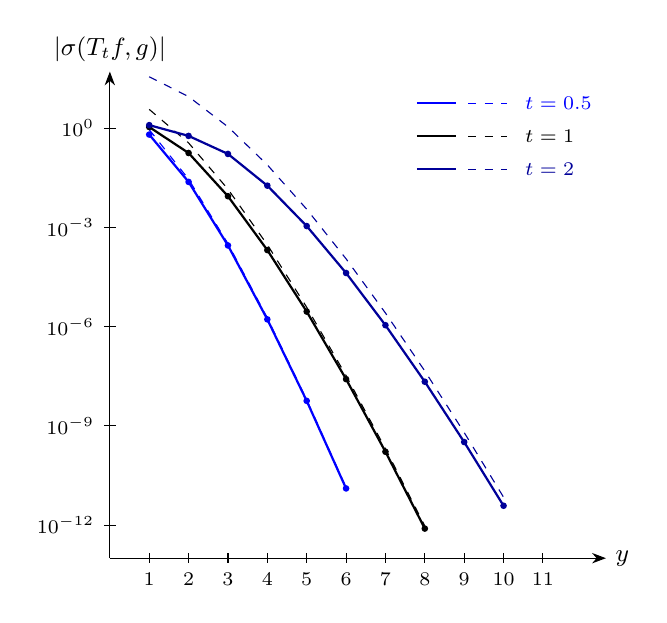
\begin{tikzpicture}[x=0.5cm,y=1cm,>={Stealth[length=5pt]}]
  \draw[->] (0,0) -- (12.6,0) node[right,font=\small] {$y$};
  \draw[->] (0,0) -- (0,6.18) node[above,font=\small] {$|\sigma(T_tf,g)|$};
  \draw (0.15,0.42) -- (-0.15,0.42) node[left,font=\scriptsize] {$10^{-12}$};
  \draw (0.15,1.68) -- (-0.15,1.68) node[left,font=\scriptsize] {$10^{-9}$};
  \draw (0.15,2.94) -- (-0.15,2.94) node[left,font=\scriptsize] {$10^{-6}$};
  \draw (0.15,4.20) -- (-0.15,4.20) node[left,font=\scriptsize] {$10^{-3}$};
  \draw (0.15,5.46) -- (-0.15,5.46) node[left,font=\scriptsize] {$10^{0}$};
  \draw (1,0.06) -- (1,-0.06) node[below,font=\scriptsize] {1};
  \draw (2,0.06) -- (2,-0.06) node[below,font=\scriptsize] {2};
  \draw (3,0.06) -- (3,-0.06) node[below,font=\scriptsize] {3};
  \draw (4,0.06) -- (4,-0.06) node[below,font=\scriptsize] {4};
  \draw (5,0.06) -- (5,-0.06) node[below,font=\scriptsize] {5};
  \draw (6,0.06) -- (6,-0.06) node[below,font=\scriptsize] {6};
  \draw (7,0.06) -- (7,-0.06) node[below,font=\scriptsize] {7};
  \draw (8,0.06) -- (8,-0.06) node[below,font=\scriptsize] {8};
  \draw (9,0.06) -- (9,-0.06) node[below,font=\scriptsize] {9};
  \draw (10,0.06) -- (10,-0.06) node[below,font=\scriptsize] {10};
  \draw (11,0.06) -- (11,-0.06) node[below,font=\scriptsize] {11};
  \draw[Blue,thick] (1,5.380) -- (2,4.779) -- (3,3.972) -- (4,3.033) -- (5,1.998) -- (6,0.886);
  \fill[Blue] (1,5.380) circle (1.2pt);
  \fill[Blue] (2,4.779) circle (1.2pt);
  \fill[Blue] (3,3.972) circle (1.2pt);
  \fill[Blue] (4,3.033) circle (1.2pt);
  \fill[Blue] (5,1.998) circle (1.2pt);
  \fill[Blue] (6,0.886) circle (1.2pt);
  \draw[Blue,dashed] (1,5.443) -- (2,4.813) -- (3,3.995) -- (4,3.051) -- (5,2.012) -- (6,0.897);
  \draw[Blue,thick] (7.8,5.78) -- (8.8,5.78);
  \draw[Blue,dashed] (9.1,5.78) -- (10.1,5.78);
  \node[Blue,anchor=west,font=\scriptsize] at (10.3,5.78) {$t=0.5$};
  \draw[black,thick] (1,5.476) -- (2,5.146) -- (3,4.597) -- (4,3.913) -- (5,3.132) -- (6,2.274) -- (7,1.352) -- (8,0.376);
  \fill[black] (1,5.476) circle (1.2pt);
  \fill[black] (2,5.146) circle (1.2pt);
  \fill[black] (3,4.597) circle (1.2pt);
  \fill[black] (4,3.913) circle (1.2pt);
  \fill[black] (5,3.132) circle (1.2pt);
  \fill[black] (6,2.274) circle (1.2pt);
  \fill[black] (7,1.352) circle (1.2pt);
  \fill[black] (8,0.376) circle (1.2pt);
  \draw[black,dashed] (1,5.700) -- (2,5.274) -- (3,4.686) -- (4,3.981) -- (5,3.187) -- (6,2.319) -- (7,1.391) -- (8,0.410);
  \draw[black,thick] (7.8,5.36) -- (8.8,5.36);
  \draw[black,dashed] (9.1,5.36) -- (10.1,5.36);
  \node[black,anchor=west,font=\scriptsize] at (10.3,5.36) {$t=1$};
  \draw[Blue!60!black,thick] (1,5.500) -- (2,5.363) -- (3,5.134) -- (4,4.731) -- (5,4.218) -- (6,3.622) -- (7,2.959) -- (8,2.241) -- (9,1.475) -- (10,0.666);
  \fill[Blue!60!black] (1,5.500) circle (1.2pt);
  \fill[Blue!60!black] (2,5.363) circle (1.2pt);
  \fill[Blue!60!black] (3,5.134) circle (1.2pt);
  \fill[Blue!60!black] (4,4.731) circle (1.2pt);
  \fill[Blue!60!black] (5,4.218) circle (1.2pt);
  \fill[Blue!60!black] (6,3.622) circle (1.2pt);
  \fill[Blue!60!black] (7,2.959) circle (1.2pt);
  \fill[Blue!60!black] (8,2.241) circle (1.2pt);
  \fill[Blue!60!black] (9,1.475) circle (1.2pt);
  \fill[Blue!60!black] (10,0.666) circle (1.2pt);
  \draw[Blue!60!black,dashed] (1,6.114) -- (2,5.862) -- (3,5.478) -- (4,4.995) -- (5,4.432) -- (6,3.802) -- (7,3.114) -- (8,2.377) -- (9,1.596) -- (10,0.775);
  \draw[Blue!60!black,thick] (7.8,4.94) -- (8.8,4.94);
  \draw[Blue!60!black,dashed] (9.1,4.94) -- (10.1,4.94);
  \node[Blue!60!black,anchor=west,font=\scriptsize] at (10.3,4.94) {$t=2$};
\end{tikzpicture}

\caption{\vetnew{The harmonic chain of twelve sites, $\omega=\lambda=1$: the exact
$\abs{\sigma(T_tf,g)}$ (solid, maximized over $f$ at the site $0$ and $g$ at the site $y$ with
coordinates of modulus at most $1$) and the entrywise bound \eqref{eq:harmonicbound} (dashed),
against $y$ on a logarithmic scale, for three times. The bound shares the decay of the exact
quantity and lies above it by a factor that grows with $t$.}}
\label{fig:harmonic}
\end{figure}

\begin{proposition}[witness]\label{prop:harmonicwitness}
\vetnew{For $\lambda>0$ and $n\ge2$, with $f=\delta_{(0,p)}$ and $g=\delta_{(1,p)}$, there is
$t>0$ with $\comm{\alpha_t(W(f))}{W(g)}\ne0$: the momenta at neighbouring sites do not commute
after evolution.}
\end{proposition}
\begin{proof}
\vetnew{$\phi(t)=\sigma(T_tf,g)$ has $\phi(0)=0$ and
$\phi'(0)=\sigma(Kf,g)=(Kf)^q_1=-A_{10}=\lambda>0$, so $0<\phi(t)<2\pi$ for small $t>0$, and the
norm $2\abs{\sin(\phi(t)/2)}$ of Theorem~\ref{thm:weylcommutator} is nonzero. For the position
pair $\delta_{(0,q)},\delta_{(1,q)}$ the first two orders vanish ($Kf$ and $K^2f$ pair with $g$
through momentum coordinates only, and $\sigma(Kf,g)=\sigma(K^2f,g)=0$) and
$\phi(t)=-\lambda t^3/6+O(t^4)$: the commutator appears at order $t^3$.}
\end{proof}

\subsection*{Notes and references}

\vetnew{\emph{The source.} The harmonic bound is Theorem~3.1 of \cite{nrss2009}: for the chain
\eqref{eq:chainH} on a periodic cube (their Hamiltonian without the factor $\tfrac12$, so their
time is half of ours; their chain is periodic where ours has open ends, and in $\nu$ dimensions
their constant carries $4\sum_j\lambda_j$), with $\supp f\subseteq X$, $\supp g\subseteq Y$ and any $\mu>0$,
\begin{gather*}
\norm{\comm{\tau_t(W(f))}{W(g)}}\le C\norm f_\infty\norm g_\infty\sum_{x\in X,\,y\in Y}
\exp\bigl(-\mu\,(d(x,y)-c_{\omega,\lambda}\max(2/\mu,e^{\mu/2+1})\abs t)\bigr),\\
c_{\omega,\lambda}=(\omega^2+4\lambda)^{1/2},
\end{gather*}
their eq.~(3.10), with $C=2+c_{\omega,\lambda}e^{\mu/2}+c_{\omega,\lambda}^{-1}$.

Their proof has the
same first two steps as ours, their Lemma~3.4 ($\tau_t(W(f))=W(f_t)$, obtained there by a
normal-mode computation) and the commutator identity \eqref{eq:weylcomm} (their p.~12 and
eq.~(3.21)); the third step differs: they bound the propagator kernel by a Fourier sum and a
power-series tail with an estimate of the factorials (their Lemmas~3.5 and 3.7), while
Theorem~\ref{thm:entrywise} bounds it entrywise by $e^{\abs t\abs K}$ and Chapter~\ref{sec:closed}'s
tail. Theorem~\ref{thm:harmonicbound} with Corollary~\ref{cor:harmonicclosed} and the paragraph
after it gives their
statement in shape: exponential decay in the distance with a linear light cone, the constants
depending on $\omega$ and $\lambda$ only.

The velocities are not the same number: in their time
unit and at the same $\mu$, our cone (the paragraph after Corollary~\ref{cor:harmonicclosed}) moves at
$2e^\mu c_{\omega,\lambda}/\mu$ after the balanced rescaling, theirs at
$c_{\omega,\lambda}\max(2/\mu,e^{\mu/2+1})$; the two agree at $\mu=2$ and ours is the larger
elsewhere, so their cone is the narrower (at the best $\mu$, $3.6\,c_{\omega,\lambda}$ against
our $5.4\,c_{\omega,\lambda}$); our prefactor has the simpler form.

\emph{The mechanism.} That the dynamics of a quadratic Hamiltonian is a symplectic flow on the
Weyl labels is classical. The bounded-density bounds
for interacting bosons are a different, state-dependent subject and are not treated in these
notes.}

\paragraph{Checks.} {\small \vetnew{The generator condition, symplecticity, the group law, the
Weyl commutator norm, the entrywise bound and the power bound, the chain of inequalities \eqref{eq:harmonicbound} on a chain of
eight sites, the light cone, the row sums before and after the rescaling with the balancing
exponent, the momentum-pair witness and the position pair's $t^3$ onset, the sharper cone tail
and the time normalisation against the source are computed by \texttt{checks/m5\_check.py}; the
numbers of Example~\ref{ex:harmonicchain} (twelve sites) and Figure~\ref{fig:harmonic} by
\texttt{checks/m5\_figure.py}.}}


\section{The thermodynamic limit}\label{sec:limit}
\vetnew{This chapter is to come.}

\section*{Notes and references}
\addcontentsline{toc}{section}{Notes and references}
\vetnew{The comparisons with the sources are in the chapters' end notes.}

\begin{thebibliography}{99}
\bibitem{chen-lucas-yin} C.-F. Chen, A. Lucas, C. Yin, Speed limits and locality in many-body
quantum dynamics, Rep. Prog. Phys. 86 (2023) 116001, arXiv:2303.07386,
\href{https://doi.org/10.1088/1361-6633/acfaae}{doi:10.1088/1361-6633/acfaae}.
\bibitem{lieb-robinson} E. H. Lieb, D. W. Robinson, The finite group velocity of quantum spin
systems, Commun. Math. Phys. 28 (1972) 251--257,
\href{https://doi.org/10.1007/BF01645779}{doi:10.1007/BF01645779}.
\bibitem{hastings-koma} M. B. Hastings, T. Koma, Spectral gap and exponential decay of
correlations, Commun. Math. Phys. 265 (2006) 781--804, arXiv:math-ph/0507008,
\href{https://doi.org/10.1007/s00220-006-0030-4}{doi:10.1007/s00220-006-0030-4}.
\bibitem{nachtergaele-sims} B. Nachtergaele, R. Sims, Lieb-Robinson bounds and the exponential
clustering theorem, Commun. Math. Phys. 265 (2006) 119--130, arXiv:math-ph/0506030,
\href{https://doi.org/10.1007/s00220-006-1556-1}{doi:10.1007/s00220-006-1556-1}.
\bibitem{nsy2018} B. Nachtergaele, R. Sims, A. Young, Lieb-Robinson bounds, the spectral flow,
and stability of the spectral gap for lattice fermion systems, in Mathematical Problems in Quantum
Physics, Contemp. Math. 717 (2018) 93--115, arXiv:1705.08553,
\href{https://doi.org/10.1090/conm/717/14443}{doi:10.1090/conm/717/14443}.
\bibitem{nsy2019} B. Nachtergaele, R. Sims, A. Young, Quasi-locality bounds for quantum lattice
systems. I. Lieb-Robinson bounds, quasi-local maps, and spectral flow automorphisms, J. Math.
Phys. 60 (2019) 061101, arXiv:1810.02428,
\href{https://doi.org/10.1063/1.5095769}{doi:10.1063/1.5095769}.
\bibitem{nrss2009} B. Nachtergaele, H. Raz, B. Schlein, R. Sims, Lieb-Robinson bounds for
harmonic and anharmonic lattice systems, Commun. Math. Phys. 286 (2009) 1073--1098,
arXiv:0712.3820,
\href{https://doi.org/10.1007/s00220-008-0630-2}{doi:10.1007/s00220-008-0630-2}.
\bibitem{chen-lucas2021} C.-F. Chen, A. Lucas, Operator growth bounds from graph theory, Commun.
Math. Phys. 385 (2021) 1273--1323, arXiv:1905.03682,
\href{https://doi.org/10.1007/s00220-021-04151-6}{doi:10.1007/s00220-021-04151-6}.
\end{thebibliography}

\clearpage
\section*{Lean declarations}\addcontentsline{toc}{section}{Lean declarations}
\noindent\vetnew{The linked \LLLeanTag{} tag marks a result whose Lean proof has been checked and whose
correspondence with the statement here has been reviewed. Definitions are listed for navigation;
only marked statements were reviewed. Files marked (in \mbox{LinearAQFT}), (in \mbox{LocalAlgebrasLean}) or (in
\mbox{BosonicLean}) belong to those libraries, on which this one depends, and the declarations listed under them are
defined there.}
\medskip

{\small
\begin{longtable}{@{}>{\raggedright\arraybackslash}p{0.19\textwidth}>{\raggedright\arraybackslash}p{0.78\textwidth}@{}}
\toprule
Statement & Declarations\\
\midrule
\endhead
\multicolumn{2}{@{}p{0.97\textwidth}@{}}{\textbf{Chapter~\ref{sec:objects}, \nameref{sec:objects}}}\\[2pt]
\multicolumn{2}{@{}>{\raggedright\arraybackslash}p{0.97\textwidth}@{}}{\textit{Files} \path{LinearAQFT/Net/Basic.lean} (in \mbox{LinearAQFT}), \path{LocalAlgebrasLean/Net/Basic.lean} (in \mbox{LocalAlgebrasLean}), \path{LocalityLean/Core/Support.lean}}\\[2pt]
\quad Definition~\ref{def:net} & \texttt{\detokenize{LinearAQFT.Net}}\newline \texttt{\detokenize{LocalAlgebrasLean.Net}}\newline \texttt{\detokenize{LinearAQFT.Net.IsCausal}}\newline \texttt{\detokenize{LocalityLean.latticeIndex}}\newline \texttt{\detokenize{LocalityLean.commute_of_isCausal_of_disjoint}}\\[3pt]
\multicolumn{2}{@{}>{\raggedright\arraybackslash}p{0.97\textwidth}@{}}{\textit{File} \path{LocalityLean/Core/Generator.lean}}\\[2pt]
\quad Definition~\ref{def:commnorm} & \texttt{\detokenize{LocalityLean.comm}}\newline \texttt{\detokenize{LocalityLean.commSet}}\newline \texttt{\detokenize{LocalityLean.commNorm}}\\[3pt]
\quad Proposition~\ref{prop:commnorm}\hypertarget{lean:prop:commnorm}{} & \texttt{\detokenize{LocalityLean.commNorm_nonneg}}\newline \texttt{\detokenize{LocalityLean.commNorm_le_two_mul_norm}}\newline \texttt{\detokenize{LocalityLean.norm_comm_le_commNorm}}\newline \texttt{\detokenize{LocalityLean.commNorm_eq_zero_of_commute}}\newline \texttt{\detokenize{LocalityLean.commNorm_mono}}\newline \texttt{\detokenize{LocalityLean.commNorm_add_le}}\newline \texttt{\detokenize{LocalityLean.commNorm_smul}}\newline \texttt{\detokenize{LocalityLean.abs_commNorm_sub_le}}\\[3pt]
\quad Definition~\ref{def:local-generators} & \texttt{\detokenize{LocalityLean.LocalGenerators}}\newline \texttt{\detokenize{LocalityLean.LocalGenerators.subfamily}}\newline \texttt{\detokenize{LocalityLean.LocalGenerators.total}}\newline \texttt{\detokenize{LocalityLean.LocalGenerators.evolve}}\newline \texttt{\detokenize{LocalityLean.LocalGenerators.totalStrength}}\newline \texttt{\detokenize{LocalityLean.Crosses}}\newline \texttt{\detokenize{LocalityLean.LocalGenerators.crosses}}\\[3pt]
\quad Proposition~\ref{prop:subfamilies}\hypertarget{lean:prop:subfamilies}{} & \texttt{\detokenize{LocalityLean.LocalGenerators.subfamily_union}}\newline \texttt{\detokenize{LocalityLean.LocalGenerators.total_eq_crosses_add_compl}}\newline \texttt{\detokenize{LocalityLean.LocalGenerators.norm_evolve_le}}\newline \texttt{\detokenize{LocalityLean.LocalGenerators.norm_subfamily_apply_le}}\\[3pt]
\multicolumn{2}{@{}>{\raggedright\arraybackslash}p{0.97\textwidth}@{}}{\textit{File} \path{LocalityLean/Core/Derivation.lean}}\\[2pt]
\quad Example~\ref{ex:hamiltonian}\hypertarget{lean:ex:hamiltonian}{} & \texttt{\detokenize{LocalityLean.Interaction.toGenerators}}\newline \texttt{\detokenize{LocalityLean.norm_derivation_apply_le}}\newline \texttt{\detokenize{LocalityLean.derivation_apply_mem}}\newline \texttt{\detokenize{LocalityLean.Interaction.norm_exp_subfamily_le_one}}\newline \texttt{\detokenize{LocalityLean.Interaction.evolve_eq_conj}}\\[3pt]
\multicolumn{2}{@{}>{\raggedright\arraybackslash}p{0.97\textwidth}@{}}{\textit{File} \path{LocalityLean/Core/Path.lean}}\\[2pt]
\quad Definition~\ref{def:path} & \texttt{\detokenize{LocalityLean.LocalGenerators.IsPath}}\newline \texttt{\detokenize{LocalityLean.LocalGenerators.pathSum}}\\[3pt]
\quad Proposition~\ref{prop:pathcount}\hypertarget{lean:prop:pathcount}{} & \texttt{\detokenize{LocalityLean.LocalGenerators.bridge}}\newline \texttt{\detokenize{LocalityLean.LocalGenerators.through}}\newline \texttt{\detokenize{LocalityLean.LocalGenerators.pathSumRec}}\newline \texttt{\detokenize{LocalityLean.LocalGenerators.pathSum_one}}\newline \texttt{\detokenize{LocalityLean.LocalGenerators.pathSum_succ_succ}}\newline \texttt{\detokenize{LocalityLean.LocalGenerators.pathSum_eq_pathSumRec}}\newline \texttt{\detokenize{LocalityLean.LocalGenerators.pathSumRec_nonneg}}\newline \texttt{\detokenize{LocalityLean.LocalGenerators.pathSumRec_le}}\\[3pt]
\multicolumn{2}{@{}p{0.97\textwidth}@{}}{\textbf{Chapter~\ref{sec:master}, \nameref{sec:master}}}\\[2pt]
\multicolumn{2}{@{}>{\raggedright\arraybackslash}p{0.97\textwidth}@{}}{\textit{Files} \path{LocalityLean/Core/Duhamel.lean}, \path{LocalityLean/Core/Bound.lean}}\\[2pt]
\quad Lemma~\ref{lem:duhamel}\hypertarget{lean:lem:duhamel}{} & \texttt{\detokenize{LocalityLean.duhamel}}\newline \texttt{\detokenize{LocalityLean.continuous_exp_smul}}\newline \texttt{\detokenize{LocalityLean.continuous_exp_sub_smul}}\newline \texttt{\detokenize{LocalityLean.LocalGenerators.continuous_duhamel_integrand}}\\[3pt]
\multicolumn{2}{@{}>{\raggedright\arraybackslash}p{0.97\textwidth}@{}}{\textit{File} \path{LocalityLean/Core/Duhamel.lean}}\\[2pt]
\quad Lemma~\ref{lem:invariance}\hypertarget{lean:lem:invariance}{} & \texttt{\detokenize{LocalityLean.exp_apply_mem_of_maps_into}}\newline \texttt{\detokenize{LocalityLean.pow_apply_mem_of_maps_into}}\\[3pt]
\multicolumn{2}{@{}>{\raggedright\arraybackslash}p{0.97\textwidth}@{}}{\textit{File} \path{LocalityLean/Core/Bound.lean}}\\[2pt]
\quad Proposition~\ref{prop:annihilate}\hypertarget{lean:prop:annihilate}{} & \texttt{\detokenize{LocalityLean.LocalGenerators.apply_eq_zero_of_subset}}\\[3pt]
\quad Proposition~\ref{prop:support}\hypertarget{lean:prop:support}{} & \texttt{\detokenize{LocalityLean.LocalGenerators.subfamily_apply_mem}}\newline \texttt{\detokenize{LocalityLean.LocalGenerators.exp_subfamily_apply_mem}}\newline \texttt{\detokenize{LocalityLean.LocalGenerators.subfamily_compl_crosses_apply_mem}}\newline \texttt{\detokenize{LocalityLean.LocalGenerators.exp_compl_crosses_apply_mem}}\\[3pt]
\quad Proposition~\ref{prop:first}\hypertarget{lean:prop:first}{} & \texttt{\detokenize{LocalityLean.LocalGenerators.comm_exp_compl_eq_zero}}\\[3pt]
\quad Proposition~\ref{prop:reset}\hypertarget{lean:prop:reset}{} & \texttt{\detokenize{LocalityLean.LocalGenerators.norm_comm_reset_le}}\\[3pt]
\quad Theorem~\ref{thm:onestep}\hypertarget{lean:thm:onestep}{} & \texttt{\detokenize{LocalityLean.LocalGenerators.norm_comm_evolve_le_of_majorant}}\\[3pt]
\multicolumn{2}{@{}>{\raggedright\arraybackslash}p{0.97\textwidth}@{}}{\textit{Files} \path{LocalityLean/Core/Bound.lean}, \path{LocalityLean/Core/Path.lean}}\\[2pt]
\quad Theorem~\ref{thm:iteration}\hypertarget{lean:thm:iteration}{} & \texttt{\detokenize{LocalityLean.LocalGenerators.coef}}\newline \texttt{\detokenize{LocalityLean.LocalGenerators.truncBound}}\newline \texttt{\detokenize{LocalityLean.LocalGenerators.integral_coef}}\newline \texttt{\detokenize{LocalityLean.LocalGenerators.norm_comm_evolve_le_truncBound}}\newline \texttt{\detokenize{LocalityLean.LocalGenerators.pathSum_eq_pathSumRec}}\\[3pt]
\multicolumn{2}{@{}>{\raggedright\arraybackslash}p{0.97\textwidth}@{}}{\textit{Files} \path{LocalityLean/Core/Bound.lean}, \path{LocalityLean/Core/Path.lean}, \path{LocalityLean/Core/Decay.lean}}\\[2pt]
\quad Theorem~\ref{thm:master}\hypertarget{lean:thm:master}{} & \texttt{\detokenize{LocalityLean.LocalGenerators.seriesTerm}}\newline \texttt{\detokenize{LocalityLean.LocalGenerators.summable_seriesTerm}}\newline \texttt{\detokenize{LocalityLean.LocalGenerators.seriesTerm_le}}\newline \texttt{\detokenize{LocalityLean.LocalGenerators.liebRobinson_path}}\newline \texttt{\detokenize{LocalityLean.LocalGenerators.liebRobinson}}\newline \texttt{\detokenize{LocalityLean.LocalGenerators.commBound}}\newline \texttt{\detokenize{LocalityLean.LocalGenerators.commBound_le}}\newline \texttt{\detokenize{LocalityLean.LocalGenerators.pathSum_eq_pathSumRec}}\newline \texttt{\detokenize{LocalityLean.tsum_pow_succ_div_factorial}}\\[3pt]
\multicolumn{2}{@{}p{0.97\textwidth}@{}}{\textbf{Chapter~\ref{sec:closed}, \nameref{sec:closed}}}\\[2pt]
\multicolumn{2}{@{}>{\raggedright\arraybackslash}p{0.97\textwidth}@{}}{\textit{File} \path{LocalityLean/Core/SiteMatrix.lean}}\\[2pt]
\quad Definition~\ref{def:sitematrix} & \texttt{\detokenize{LocalityLean.LocalGenerators.touched}}\newline \texttt{\detokenize{LocalityLean.LocalGenerators.ind}}\newline \texttt{\detokenize{LocalityLean.LocalGenerators.siteMatrix}}\newline \texttt{\detokenize{LocalityLean.LocalGenerators.walk}}\newline \texttt{\detokenize{LocalityLean.LocalGenerators.boundary}}\newline \texttt{\detokenize{LocalityLean.LocalGenerators.regionSites}}\newline \texttt{\detokenize{LocalityLean.LocalGenerators.walkSum}}\\[3pt]
\quad Proposition~\ref{prop:walkprops}\hypertarget{lean:prop:walkprops}{} & \texttt{\detokenize{LocalityLean.LocalGenerators.weightedSize}}\newline \texttt{\detokenize{LocalityLean.LocalGenerators.siteMatrix_nonneg}}\newline \texttt{\detokenize{LocalityLean.LocalGenerators.siteMatrix_comm}}\newline \texttt{\detokenize{LocalityLean.LocalGenerators.siteMatrix_eq_zero_of_not_mem_left}}\newline \texttt{\detokenize{LocalityLean.LocalGenerators.siteMatrix_eq_zero_of_not_mem_right}}\newline \texttt{\detokenize{LocalityLean.LocalGenerators.sum_siteMatrix_le}}\newline \texttt{\detokenize{LocalityLean.LocalGenerators.walk_nonneg}}\newline \texttt{\detokenize{LocalityLean.LocalGenerators.walk_eq_zero_of_not_mem_left}}\newline \texttt{\detokenize{LocalityLean.LocalGenerators.walk_eq_zero_of_not_mem_right}}\newline \texttt{\detokenize{LocalityLean.LocalGenerators.walk_one_of_mem}}\newline \texttt{\detokenize{LocalityLean.LocalGenerators.sum_walk_le_of_rowSum}}\newline \texttt{\detokenize{LocalityLean.LocalGenerators.sum_walk_le}}\newline \texttt{\detokenize{LocalityLean.LocalGenerators.walkSum_le_of_rowSum}}\newline \texttt{\detokenize{LocalityLean.LocalGenerators.walkSum_le}}\\[3pt]
\multicolumn{2}{@{}>{\raggedright\arraybackslash}p{0.97\textwidth}@{}}{\textit{Files} \path{LocalityLean/Core/SiteMatrix.lean}, \path{LocalityLean/Core/Path.lean}}\\[2pt]
\quad Theorem~\ref{thm:domination}\hypertarget{lean:thm:domination}{} & \texttt{\detokenize{LocalityLean.LocalGenerators.pathSumRec_one_le_walkSum}}\newline \texttt{\detokenize{LocalityLean.LocalGenerators.walkSum_succ_eq}}\newline \texttt{\detokenize{LocalityLean.LocalGenerators.pathSumRec_le_walkSum}}\newline \texttt{\detokenize{LocalityLean.LocalGenerators.pathSum_eq_pathSumRec}}\\[3pt]
\multicolumn{2}{@{}>{\raggedright\arraybackslash}p{0.97\textwidth}@{}}{\textit{Files} \path{LocalityLean/Core/SiteMatrix.lean}, \path{LocalityLean/Core/Decay.lean}}\\[2pt]
\quad Theorem~\ref{thm:walkseries}\hypertarget{lean:thm:walkseries}{} & \texttt{\detokenize{LocalityLean.LocalGenerators.walkTerm}}\newline \texttt{\detokenize{LocalityLean.LocalGenerators.summable_walkTerm}}\newline \texttt{\detokenize{LocalityLean.LocalGenerators.walkTerm_le}}\newline \texttt{\detokenize{LocalityLean.LocalGenerators.tsum_seriesTerm_le_tsum_walkTerm}}\newline \texttt{\detokenize{LocalityLean.LocalGenerators.liebRobinson_walk}}\newline \texttt{\detokenize{LocalityLean.LocalGenerators.commBound_le_walk}}\newline \texttt{\detokenize{LocalityLean.tsum_pow_succ_div_factorial}}\\[3pt]
\multicolumn{2}{@{}>{\raggedright\arraybackslash}p{0.97\textwidth}@{}}{\textit{File} \path{LocalityLean/Core/SiteMatrix.lean}}\\[2pt]
\quad Proposition~\ref{prop:finite}\hypertarget{lean:prop:finite}{} & \texttt{\detokenize{LocalityLean.LocalGenerators.toMatrix}}\newline \texttt{\detokenize{LocalityLean.LocalGenerators.walk_eq_pow_apply}}\newline \texttt{\detokenize{LocalityLean.LocalGenerators.hasSum_exp_apply}}\newline \texttt{\detokenize{LocalityLean.LocalGenerators.tsum_exp_apply_succ}}\newline \texttt{\detokenize{LocalityLean.LocalGenerators.tsum_walkTerm_eq}}\newline \texttt{\detokenize{LocalityLean.LocalGenerators.liebRobinson_matrixExp}}\\[3pt]
\multicolumn{2}{@{}>{\raggedright\arraybackslash}p{0.97\textwidth}@{}}{\textit{File} \path{LocalityLean/Core/Decay.lean}}\\[2pt]
\quad Definition~\ref{def:kernel} & \texttt{\detokenize{LocalityLean.DecayKernel}}\newline \texttt{\detokenize{LocalityLean.LocalGenerators.IsFBound}}\newline \texttt{\detokenize{LocalityLean.LocalGenerators.kernelSum}}\\[3pt]
\quad Theorem~\ref{thm:decay}\hypertarget{lean:thm:decay}{} & \texttt{\detokenize{LocalityLean.LocalGenerators.walk_le_decay}}\newline \texttt{\detokenize{LocalityLean.LocalGenerators.walkSum_le_decay}}\newline \texttt{\detokenize{LocalityLean.LocalGenerators.tsum_walkTerm_le_decay}}\newline \texttt{\detokenize{LocalityLean.LocalGenerators.liebRobinson_decay}}\\[3pt]
\quad Definition~\ref{def:geometry} & \texttt{\detokenize{LocalityLean.LocalGenerators.degreeAt}}\newline \texttt{\detokenize{LocalityLean.LocalGenerators.BoundedGeometry}}\newline \texttt{\detokenize{LocalityLean.LocalGenerators.BoundedGeometry.M}}\newline \texttt{\detokenize{LocalityLean.LocalGenerators.BoundedGeometry.v}}\\[3pt]
\multicolumn{2}{@{}>{\raggedright\arraybackslash}p{0.97\textwidth}@{}}{\textit{Files} \path{LocalityLean/Core/Decay.lean}, \path{LocalityLean/Core/SiteMatrix.lean}}\\[2pt]
\quad Proposition~\ref{prop:distance}\hypertarget{lean:prop:distance}{} & \texttt{\detokenize{LocalityLean.LocalGenerators.BoundedGeometry.walk_eq_zero_of_dist}}\newline \texttt{\detokenize{LocalityLean.LocalGenerators.BoundedGeometry.sum_siteMatrix_le}}\newline \texttt{\detokenize{LocalityLean.LocalGenerators.walkSum_le_of_rowSum}}\\[3pt]
\multicolumn{2}{@{}>{\raggedright\arraybackslash}p{0.97\textwidth}@{}}{\textit{File} \path{LocalityLean/Core/Decay.lean}}\\[2pt]
\quad Lemma~\ref{lem:tail}\hypertarget{lean:lem:tail}{} & \texttt{\detokenize{LocalityLean.factorial_mul_factorial_le}}\newline \texttt{\detokenize{LocalityLean.tsum_pow_div_factorial_tail_le}}\\[3pt]
\quad Theorem~\ref{thm:geometry}\hypertarget{lean:thm:geometry}{} & \texttt{\detokenize{LocalityLean.LocalGenerators.BoundedGeometry.walkSum_eq_zero_of_dist}}\newline \texttt{\detokenize{LocalityLean.LocalGenerators.BoundedGeometry.tsum_walkTerm_le_geom}}\newline \texttt{\detokenize{LocalityLean.LocalGenerators.liebRobinson_boundedGeometry}}\\[3pt]
\quad Theorem~\ref{thm:cone}\hypertarget{lean:thm:cone}{} & \texttt{\detokenize{LocalityLean.pow_div_factorial_le_exp_sub}}\newline \texttt{\detokenize{LocalityLean.LocalGenerators.liebRobinson_cone}}\\[3pt]
\multicolumn{2}{@{}>{\raggedright\arraybackslash}p{0.97\textwidth}@{}}{\textit{File} \path{LocalityLean/Core/Reverse.lean}}\\[2pt]
\quad Theorem~\ref{thm:reverse}\hypertarget{lean:thm:reverse}{} & \texttt{\detokenize{LocalityLean.LocalGenerators.NegContractive}}\newline \texttt{\detokenize{LocalityLean.LocalGenerators.neg}}\newline \texttt{\detokenize{LocalityLean.LocalGenerators.neg_evolve}}\newline \texttt{\detokenize{LocalityLean.LocalGenerators.liebRobinson_abs}}\newline \texttt{\detokenize{LocalityLean.LocalGenerators.liebRobinson_walk_abs}}\newline \texttt{\detokenize{LocalityLean.LocalGenerators.liebRobinson_decay_abs}}\\[3pt]
\multicolumn{2}{@{}p{0.97\textwidth}@{}}{\textbf{Chapter~\ref{sec:qudit}, \nameref{sec:qudit}}}\\[2pt]
\multicolumn{2}{@{}>{\raggedright\arraybackslash}p{0.97\textwidth}@{}}{\textit{File} \path{LocalityLean/Core/Derivation.lean}}\\[2pt]
\quad Definition~\ref{def:hamfamily} & \texttt{\detokenize{LocalityLean.derivation}}\newline \texttt{\detokenize{LocalityLean.derivation_apply}}\newline \texttt{\detokenize{LocalityLean.Interaction}}\newline \texttt{\detokenize{LocalityLean.Interaction.hamiltonian}}\newline \texttt{\detokenize{LocalityLean.Interaction.derivation_hamiltonian}}\\[3pt]
\quad Proposition~\ref{prop:derivation}\hypertarget{lean:prop:derivation}{} & \texttt{\detokenize{LocalityLean.norm_derivation_apply_le}}\newline \texttt{\detokenize{LocalityLean.derivation_apply_mem}}\\[3pt]
\quad Proposition~\ref{prop:expmul}\hypertarget{lean:prop:expmul}{} & \texttt{\detokenize{LocalityLean.exp_mul_clm}}\newline \texttt{\detokenize{LocalityLean.exp_mul_clm_flip}}\newline \texttt{\detokenize{LocalityLean.commute_mul_clm_flip}}\newline \texttt{\detokenize{LocalityLean.exp_mul_clm_add_flip_apply}}\\[3pt]
\quad Proposition~\ref{prop:conjugation}\hypertarget{lean:prop:conjugation}{} & \texttt{\detokenize{LocalityLean.exp_I_smul_mem_unitary}}\newline \texttt{\detokenize{LocalityLean.star_exp_I_smul}}\newline \texttt{\detokenize{LocalityLean.exp_smul_derivation_apply_eq_conj}}\newline \texttt{\detokenize{LocalityLean.norm_exp_smul_derivation_apply}}\\[3pt]
\multicolumn{2}{@{}>{\raggedright\arraybackslash}p{0.97\textwidth}@{}}{\textit{Files} \path{LocalityLean/Core/Derivation.lean}, \path{LocalityLean/Core/Reverse.lean}}\\[2pt]
\quad Theorem~\ref{thm:hamgenerators}\hypertarget{lean:thm:hamgenerators}{} & \texttt{\detokenize{LocalityLean.Interaction.toGenerators}}\newline \texttt{\detokenize{LocalityLean.Interaction.toGenerators_kappa}}\newline \texttt{\detokenize{LocalityLean.Interaction.toGenerators_negContractive}}\newline \texttt{\detokenize{LocalityLean.Interaction.unitaryAt}}\newline \texttt{\detokenize{LocalityLean.Interaction.star_unitaryAt}}\newline \texttt{\detokenize{LocalityLean.Interaction.evolve_eq_conj}}\newline \texttt{\detokenize{LocalityLean.LocalGenerators.liebRobinson_abs}}\newline \texttt{\detokenize{LocalityLean.LocalGenerators.liebRobinson_walk_abs}}\newline \texttt{\detokenize{LocalityLean.LocalGenerators.liebRobinson_decay_abs}}\\[3pt]
\multicolumn{2}{@{}>{\raggedright\arraybackslash}p{0.97\textwidth}@{}}{\textit{File} \path{LocalityLean/Core/Derivation.lean}}\\[2pt]
\quad Theorem~\ref{thm:exchange}\hypertarget{lean:thm:exchange}{} & \texttt{\detokenize{LocalityLean.Interaction.comm_conj_eq}}\newline \texttt{\detokenize{LocalityLean.Interaction.norm_comm_conj_eq}}\newline \texttt{\detokenize{LocalityLean.Interaction.norm_comm_evolve_eq}}\newline \texttt{\detokenize{LocalityLean.Interaction.liebRobinson_walk_exchange}}\newline \texttt{\detokenize{LocalityLean.Interaction.liebRobinson_walk_min}}\newline \texttt{\detokenize{LocalityLean.Interaction.liebRobinson_decay_exchange}}\newline \texttt{\detokenize{LocalityLean.Interaction.liebRobinson_decay_min}}\\[3pt]
\multicolumn{2}{@{}>{\raggedright\arraybackslash}p{0.97\textwidth}@{}}{\textit{File} \path{LocalAlgebrasLean/Qudit/Config.lean} (in \mbox{LocalAlgebrasLean})}\\[2pt]
\quad Definition~\ref{def:localmatrix} & \texttt{\detokenize{LocalAlgebrasLean.Qudit.Config}}\newline \texttt{\detokenize{LocalAlgebrasLean.Qudit.AgreesOff}}\newline \texttt{\detokenize{LocalAlgebrasLean.Qudit.restrict}}\newline \texttt{\detokenize{LocalAlgebrasLean.Qudit.glue}}\newline \texttt{\detokenize{LocalAlgebrasLean.Qudit.QuditAlgebra}}\newline \texttt{\detokenize{LocalAlgebrasLean.Qudit.IsLocal}}\newline \texttt{\detokenize{LocalAlgebrasLean.Qudit.localAlgebra}}\newline \texttt{\detokenize{LocalAlgebrasLean.Qudit.embed}}\newline \texttt{\detokenize{LocalAlgebrasLean.Qudit.embed_apply}}\\[3pt]
\quad Lemma~\ref{lem:glue}\hypertarget{lean:lem:glue}{} & \texttt{\detokenize{LocalAlgebrasLean.Qudit.sum_glue}}\\[3pt]
\quad Proposition~\ref{prop:localalgebra}\hypertarget{lean:prop:localalgebra}{} & \texttt{\detokenize{LocalAlgebrasLean.Qudit.isLocal_one}}\newline \texttt{\detokenize{LocalAlgebrasLean.Qudit.IsLocal.add}}\newline \texttt{\detokenize{LocalAlgebrasLean.Qudit.IsLocal.smul}}\newline \texttt{\detokenize{LocalAlgebrasLean.Qudit.IsLocal.mul}}\newline \texttt{\detokenize{LocalAlgebrasLean.Qudit.IsLocal.star}}\newline \texttt{\detokenize{LocalAlgebrasLean.Qudit.localAlgebra_isClosed}}\newline \texttt{\detokenize{LocalAlgebrasLean.Qudit.isLocal_embed}}\newline \texttt{\detokenize{LocalAlgebrasLean.Qudit.embed_mem}}\newline \texttt{\detokenize{LocalAlgebrasLean.Qudit.isLocal_iff_exists_embed}}\newline \texttt{\detokenize{LocalAlgebrasLean.Qudit.localAlgebra_mono}}\newline \texttt{\detokenize{LocalAlgebrasLean.Qudit.localAlgebra_univ}}\\[3pt]
\multicolumn{2}{@{}>{\raggedright\arraybackslash}p{0.97\textwidth}@{}}{\textit{Files} \path{LocalAlgebrasLean/Qudit/Config.lean} (in \mbox{LocalAlgebrasLean}), \path{LocalityLean/Qudit/Config.lean}}\\[2pt]
\quad Theorem~\ref{thm:quditnet}\hypertarget{lean:thm:quditnet}{} & \texttt{\detokenize{LocalAlgebrasLean.Qudit.quditNet}}\newline \texttt{\detokenize{LocalAlgebrasLean.Qudit.commute_of_disjoint}}\newline \texttt{\detokenize{LocalAlgebrasLean.Qudit.quditNet_isLocallyCommutative}}\newline \texttt{\detokenize{LocalityLean.Qudit.quditNet_isCausal}}\\[3pt]
\multicolumn{2}{@{}>{\raggedright\arraybackslash}p{0.97\textwidth}@{}}{\textit{File} \path{LocalityLean/Qudit/Bounds.lean}}\\[2pt]
\quad Definition~\ref{def:quditinteraction} & \texttt{\detokenize{LocalityLean.Qudit.QuditInteraction}}\newline \texttt{\detokenize{LocalityLean.Qudit.QuditInteraction.term}}\newline \texttt{\detokenize{LocalityLean.Qudit.isSelfAdjoint_embed}}\newline \texttt{\detokenize{LocalityLean.Qudit.QuditInteraction.toInteraction}}\newline \texttt{\detokenize{LocalityLean.Qudit.QuditInteraction.toGenerators}}\\[3pt]
\multicolumn{2}{@{}>{\raggedright\arraybackslash}p{0.97\textwidth}@{}}{\textit{Files} \path{LocalityLean/Qudit/Bounds.lean}, \path{LocalityLean/Core/Derivation.lean}}\\[2pt]
\quad Theorem~\ref{thm:quditbounds}\hypertarget{lean:thm:quditbounds}{} & \texttt{\detokenize{LocalityLean.Qudit.QuditInteraction.toGenerators_negContractive}}\newline \texttt{\detokenize{LocalityLean.Qudit.QuditInteraction.evolve_eq_conj}}\newline \texttt{\detokenize{LocalityLean.Qudit.QuditInteraction.liebRobinson_walk}}\newline \texttt{\detokenize{LocalityLean.LocalGenerators.liebRobinson_matrixExp_abs}}\newline \texttt{\detokenize{LocalityLean.Qudit.QuditInteraction.liebRobinson_matrixExp}}\newline \texttt{\detokenize{LocalityLean.Qudit.QuditInteraction.liebRobinson_decay}}\newline \texttt{\detokenize{LocalityLean.Qudit.QuditInteraction.liebRobinson_boundedGeometry}}\newline \texttt{\detokenize{LocalityLean.Qudit.QuditInteraction.liebRobinson_cone}}\newline \texttt{\detokenize{LocalityLean.Interaction.norm_comm_evolve_eq}}\\[3pt]
\multicolumn{2}{@{}>{\raggedright\arraybackslash}p{0.97\textwidth}@{}}{\textit{File} \path{LocalityLean/Qudit/Bounds.lean}}\\[2pt]
\quad Proposition~\ref{prop:fnorm}\hypertarget{lean:prop:fnorm}{} & \texttt{\detokenize{LocalityLean.LocalGenerators.fNorm}}\newline \texttt{\detokenize{LocalityLean.LocalGenerators.div_le_fNorm}}\newline \texttt{\detokenize{LocalityLean.LocalGenerators.isFBound_fNorm}}\newline \texttt{\detokenize{LocalityLean.LocalGenerators.fNorm_le_of_isFBound}}\newline \texttt{\detokenize{LocalityLean.DecayKernel.expWeight}}\newline \texttt{\detokenize{LocalityLean.DecayKernel.expWeight_F}}\newline \texttt{\detokenize{LocalityLean.DecayKernel.expWeight_CF}}\\[3pt]
\multicolumn{2}{@{}p{0.97\textwidth}@{}}{\textbf{Chapter~\ref{sec:approx}, \nameref{sec:approx}}}\\[2pt]
\multicolumn{2}{@{}>{\raggedright\arraybackslash}p{0.97\textwidth}@{}}{\textit{File} \path{LocalityLean/Approx/LocalApprox.lean}}\\[2pt]
\quad Definition~\ref{def:localapprox} & \texttt{\detokenize{LocalityLean.LocalApprox}}\newline \texttt{\detokenize{LocalityLean.IsApproxLocalWith}}\\[3pt]
\quad Proposition~\ref{prop:converse}\hypertarget{lean:prop:converse}{} & \texttt{\detokenize{LocalityLean.commNorm_le_two_mul_norm_sub}}\newline \texttt{\detokenize{LocalityLean.LocalApprox.commNorm_compl_le}}\newline \texttt{\detokenize{LocalityLean.isApproxLocalWith_zero_iff}}\\[3pt]
\multicolumn{2}{@{}>{\raggedright\arraybackslash}p{0.97\textwidth}@{}}{\textit{File} \path{LocalityLean/Approx/Twirl.lean}}\\[2pt]
\quad Definition~\ref{def:condexp} & \texttt{\detokenize{LocalityLean.Qudit.condExp}}\newline \texttt{\detokenize{LocalityLean.Qudit.condExp_apply}}\\[3pt]
\quad Proposition~\ref{prop:condexp}\hypertarget{lean:prop:condexp}{} & \texttt{\detokenize{LocalityLean.Qudit.isLocal_condExp}}\newline \texttt{\detokenize{LocalityLean.Qudit.condExp_mem}}\newline \texttt{\detokenize{LocalityLean.Qudit.condExp_of_isLocal}}\newline \texttt{\detokenize{LocalityLean.Qudit.condExp_condExp}}\newline \texttt{\detokenize{LocalityLean.Qudit.condExp_add}}\newline \texttt{\detokenize{LocalityLean.Qudit.condExp_smul}}\newline \texttt{\detokenize{LocalityLean.Qudit.condExp_one}}\newline \texttt{\detokenize{LocalityLean.Qudit.star_condExp}}\newline \texttt{\detokenize{LocalityLean.Qudit.condExp_univ}}\newline \texttt{\detokenize{LocalityLean.Qudit.condExp_empty}}\\[3pt]
\quad Proposition~\ref{prop:clockshift}\hypertarget{lean:prop:clockshift}{} & \texttt{\detokenize{LocalityLean.Qudit.chi}}\newline \texttt{\detokenize{LocalityLean.Qudit.charSum}}\newline \texttt{\detokenize{LocalityLean.Qudit.clock}}\newline \texttt{\detokenize{LocalityLean.Qudit.shift}}\newline \texttt{\detokenize{LocalityLean.Qudit.clock_mul_shift}}\newline \texttt{\detokenize{LocalityLean.Qudit.shift_mul_star}}\\[3pt]
\quad Definition~\ref{def:weyl} & \texttt{\detokenize{LocalityLean.Qudit.shiftBy}}\newline \texttt{\detokenize{LocalityLean.Qudit.phase}}\newline \texttt{\detokenize{LocalityLean.Qudit.weyl}}\newline \texttt{\detokenize{LocalityLean.Qudit.weyl_apply}}\newline \texttt{\detokenize{LocalityLean.Qudit.twirl}}\\[3pt]
\quad Proposition~\ref{prop:weyl}\hypertarget{lean:prop:weyl}{} & \texttt{\detokenize{LocalityLean.Qudit.isLocal_weyl}}\newline \texttt{\detokenize{LocalityLean.Qudit.weyl_mem}}\newline \texttt{\detokenize{LocalityLean.Qudit.star_weyl_mul_weyl}}\newline \texttt{\detokenize{LocalityLean.Qudit.weyl_mul_star_weyl}}\newline \texttt{\detokenize{LocalityLean.Qudit.weyl_mem_unitary}}\newline \texttt{\detokenize{LocalityLean.Qudit.weyl_conj_apply}}\newline \texttt{\detokenize{LocalityLean.Qudit.phase_shiftBy_mul_star}}\\[3pt]
\quad Theorem~\ref{thm:twirl}\hypertarget{lean:thm:twirl}{} & \texttt{\detokenize{LocalityLean.Qudit.sum_phase}}\newline \texttt{\detokenize{LocalityLean.Qudit.twirl_eq_condExp}}\\[3pt]
\quad Proposition~\ref{prop:bimodule}\hypertarget{lean:prop:bimodule}{} & \texttt{\detokenize{LocalityLean.Qudit.norm_twirl_le}}\newline \texttt{\detokenize{LocalityLean.Qudit.norm_condExp_le}}\newline \texttt{\detokenize{LocalityLean.Qudit.condExp_mul_left}}\newline \texttt{\detokenize{LocalityLean.Qudit.condExp_mul_right}}\\[3pt]
\quad Theorem~\ref{thm:localapprox}\hypertarget{lean:thm:localapprox}{} & \texttt{\detokenize{LocalityLean.Qudit.norm_sub_twirl_le_commNorm}}\newline \texttt{\detokenize{LocalityLean.Qudit.norm_sub_condExp_le_commNorm}}\newline \texttt{\detokenize{LocalityLean.Qudit.commNorm_compl_le_two_mul_norm_sub_condExp}}\newline \texttt{\detokenize{LocalityLean.Qudit.localApprox}}\\[3pt]
\multicolumn{2}{@{}>{\raggedright\arraybackslash}p{0.97\textwidth}@{}}{\textit{Files} \path{LocalityLean/Approx/Truncated.lean}, \path{LocalityLean/Approx/LocalApprox.lean}, \path{LocalityLean/Core/Decay.lean}}\\[2pt]
\quad Theorem~\ref{thm:truncated}\hypertarget{lean:thm:truncated}{} & \texttt{\detokenize{LocalityLean.LocalGenerators.commNorm_evolve_le}}\newline \texttt{\detokenize{LocalityLean.LocalGenerators.norm_sub_P_evolve_le}}\newline \texttt{\detokenize{LocalityLean.LocalGenerators.norm_sub_P_evolve_le_geom}}\newline \texttt{\detokenize{LocalityLean.LocalGenerators.norm_sub_P_evolve_le_cone}}\newline \texttt{\detokenize{LocalityLean.Qudit.QuditInteraction.norm_sub_condExp_evolve_le}}\newline \texttt{\detokenize{LocalityLean.Qudit.QuditInteraction.norm_sub_condExp_evolve_le_geom}}\newline \texttt{\detokenize{LocalityLean.Qudit.QuditInteraction.norm_sub_condExp_evolve_le_cone}}\newline \texttt{\detokenize{LocalityLean.LocalApprox.norm_sub_P_le}}\newline \texttt{\detokenize{LocalityLean.LocalGenerators.BoundedGeometry.tsum_walkTerm_le_geom}}\newline \texttt{\detokenize{LocalityLean.pow_div_factorial_le_exp_sub}}\\[3pt]
\multicolumn{2}{@{}>{\raggedright\arraybackslash}p{0.97\textwidth}@{}}{\textit{File} \path{LocalityLean/Approx/Truncated.lean}}\\[2pt]
\quad Corollary~\ref{cor:automaton}\hypertarget{lean:cor:automaton}{} & \texttt{\detokenize{LocalityLean.LocalGenerators.truncError}}\newline \texttt{\detokenize{LocalityLean.LocalGenerators.evolve_isApproxLocalWith}}\newline \texttt{\detokenize{LocalityLean.LocalGenerators.neighbourhood}}\newline \texttt{\detokenize{LocalityLean.LocalGenerators.subset_neighbourhood}}\newline \texttt{\detokenize{LocalityLean.LocalGenerators.evolve_isApproxLocalWith_geom}}\newline \texttt{\detokenize{LocalityLean.LocalGenerators.evolve_isApproxLocalWith_cone}}\newline \texttt{\detokenize{LocalityLean.Qudit.QuditInteraction.evolve_isApproxLocalWith_geom}}\newline \texttt{\detokenize{LocalityLean.Qudit.QuditInteraction.evolve_isApproxLocalWith_cone}}\\[3pt]
\multicolumn{2}{@{}>{\raggedright\arraybackslash}p{0.97\textwidth}@{}}{\textit{File} \path{LocalityLean/Approx/Lindblad.lean}}\\[2pt]
\quad Definition~\ref{def:lindbladterm} & \texttt{\detokenize{LocalityLean.LindbladTerm}}\newline \texttt{\detokenize{LocalityLean.LindbladTerm.jump}}\newline \texttt{\detokenize{LocalityLean.LindbladTerm.gen}}\newline \texttt{\detokenize{LocalityLean.LindbladFamily}}\\[3pt]
\quad Proposition~\ref{prop:lindbladterm}\hypertarget{lean:prop:lindbladterm}{} & \texttt{\detokenize{LocalityLean.LindbladTerm.norm_gen_le}}\newline \texttt{\detokenize{LocalityLean.LindbladTerm.gen_apply_eq_zero_of_mem_compl}}\newline \texttt{\detokenize{LocalityLean.LindbladTerm.gen_apply_mem}}\newline \texttt{\detokenize{LocalityLean.LindbladTerm.star_gen_apply}}\\[3pt]
\quad Theorem~\ref{thm:lindbladG1}\hypertarget{lean:thm:lindbladG1}{} & \texttt{\detokenize{LocalityLean.LindbladTerm.jump_apply_eq_comm}}\newline \texttt{\detokenize{LocalityLean.LindbladTerm.norm_comm_le_norm_mul_commNorm}}\newline \texttt{\detokenize{LocalityLean.LindbladTerm.norm_jump_apply_le_commNorm}}\newline \texttt{\detokenize{LocalityLean.LindbladTerm.strengthDirect}}\newline \texttt{\detokenize{LocalityLean.LindbladTerm.norm_gen_apply_le_direct}}\newline \texttt{\detokenize{LocalityLean.LindbladTerm.gen_apply_eq_gen_sub}}\newline \texttt{\detokenize{LocalityLean.LindbladTerm.norm_gen_apply_le}}\newline \texttt{\detokenize{LocalityLean.LindbladTerm.strength}}\newline \texttt{\detokenize{LocalityLean.LindbladTerm.norm_gen_apply_le_strength}}\\[3pt]
\multicolumn{2}{@{}>{\raggedright\arraybackslash}p{0.97\textwidth}@{}}{\textit{Files} \path{LocalityLean/Approx/Lindblad.lean}, \path{LocalityLean/Core/Bound.lean}, \path{LocalityLean/Core/SiteMatrix.lean}, \path{LocalityLean/Core/Decay.lean}, \path{LocalityLean/Approx/Truncated.lean}, \path{LocalityLean/Approx/LocalApprox.lean}}\\[2pt]
\quad Theorem~\ref{thm:opensystems}\hypertarget{lean:thm:opensystems}{} & \texttt{\detokenize{LocalityLean.LindbladFamily.toGeneratorsDirect}}\newline \texttt{\detokenize{LocalityLean.LindbladFamily.toGenerators}}\newline \texttt{\detokenize{LocalityLean.LindbladFamily.toGeneratorsExplicit}}\newline \texttt{\detokenize{LocalityLean.LindbladFamily.liebRobinson_walk_direct}}\newline \texttt{\detokenize{LocalityLean.LindbladFamily.liebRobinson_walk}}\newline \texttt{\detokenize{LocalityLean.LindbladFamily.liebRobinson_cone}}\newline \texttt{\detokenize{LocalityLean.LindbladFamily.norm_sub_P_evolve_le}}\newline \texttt{\detokenize{LocalityLean.LocalGenerators.liebRobinson}}\newline \texttt{\detokenize{LocalityLean.LocalGenerators.liebRobinson_walk}}\newline \texttt{\detokenize{LocalityLean.LocalGenerators.liebRobinson_decay}}\newline \texttt{\detokenize{LocalityLean.LocalGenerators.liebRobinson_boundedGeometry}}\newline \texttt{\detokenize{LocalityLean.LocalGenerators.liebRobinson_cone}}\newline \texttt{\detokenize{LocalityLean.LocalGenerators.norm_sub_P_evolve_le}}\newline \texttt{\detokenize{LocalityLean.LocalGenerators.commNorm_evolve_le}}\newline \texttt{\detokenize{LocalityLean.LocalApprox.norm_sub_P_le}}\newline \texttt{\detokenize{LocalityLean.LocalGenerators.norm_sub_P_evolve_le_geom}}\newline \texttt{\detokenize{LocalityLean.LocalGenerators.norm_sub_P_evolve_le_cone}}\\[3pt]
\multicolumn{2}{@{}>{\raggedright\arraybackslash}p{0.97\textwidth}@{}}{\textit{File} \path{LocalityLean/Approx/Lindblad.lean}}\\[2pt]
\quad Proposition~\ref{prop:dephasing}\hypertarget{lean:prop:dephasing}{} & \texttt{\detokenize{LocalityLean.LindbladTerm.jump_eq_of_sq_eq_one}}\newline \texttt{\detokenize{LocalityLean.LindbladTerm.jump_sq}}\newline \texttt{\detokenize{LocalityLean.LindbladTerm.jump_pow_succ}}\newline \texttt{\detokenize{LocalityLean.LindbladTerm.exp_smul_jump_eq}}\newline \texttt{\detokenize{LocalityLean.LindbladTerm.exp_smul_jump_apply}}\newline \texttt{\detokenize{LocalityLean.LindbladTerm.norm_exp_smul_jump_le_one}}\\[3pt]
\multicolumn{2}{@{}>{\raggedright\arraybackslash}p{0.97\textwidth}@{}}{\textit{Files} \path{LocalityLean/Approx/Witness.lean}, \path{LocalityLean/Qudit/Witness.lean}}\\[2pt]
\quad Example~\ref{ex:dephasing}\hypertarget{lean:ex:dephasing}{} & \texttt{\detokenize{LocalityLean.Qudit.TwoQubit.dephasingTerm}}\newline \texttt{\detokenize{LocalityLean.Qudit.TwoQubit.dephasingTerm_gen_obsA}}\newline \texttt{\detokenize{LocalityLean.hasDerivAt_comm_exp}}\newline \texttt{\detokenize{LocalityLean.Qudit.TwoQubit.exists_comm_exp_ne_zero}}\newline \texttt{\detokenize{LocalityLean.Qudit.TwoQubit.comm_comm_ne_zero}}\\[3pt]
\multicolumn{2}{@{}p{0.97\textwidth}@{}}{\textbf{Chapter~\ref{sec:harmonic}, \nameref{sec:harmonic}}}\\[2pt]
\multicolumn{2}{@{}>{\raggedright\arraybackslash}p{0.97\textwidth}@{}}{\textit{Files} \path{LocalityLean/Bosonic/Phase.lean}, \path{BosonicLean/Weyl/System.lean} (in \mbox{BosonicLean}), \path{BosonicLean/Weyl/Basic.lean} (in \mbox{BosonicLean}), \path{BosonicLean/Weyl/State.lean} (in \mbox{BosonicLean})}\\[2pt]
\quad Definition~\ref{def:weylsystem} & \texttt{\detokenize{LocalityLean.Bosonic.Phase}}\newline \texttt{\detokenize{LocalityLean.Bosonic.Omega}}\newline \texttt{\detokenize{LocalityLean.Bosonic.sigma}}\newline \texttt{\detokenize{LocalityLean.Bosonic.sigma_apply}}\newline \texttt{\detokenize{BosonicLean.Weyl.WeylSystem}}\newline \texttt{\detokenize{BosonicLean.Weyl.CCR}}\newline \texttt{\detokenize{BosonicLean.Weyl.wCCR}}\newline \texttt{\detokenize{BosonicLean.Weyl.CCR.weylSystem}}\\[3pt]
\multicolumn{2}{@{}>{\raggedright\arraybackslash}p{0.97\textwidth}@{}}{\textit{Files} \path{LocalityLean/Bosonic/Phase.lean}, \path{LinearAQFT/Symplectic/Net.lean} (in \mbox{LinearAQFT})}\\[2pt]
\quad Definition~\ref{def:bosonicnet} & \texttt{\detokenize{LocalityLean.Bosonic.SuppIn}}\newline \texttt{\detokenize{LocalityLean.Bosonic.loc}}\newline \texttt{\detokenize{LocalityLean.Bosonic.phaseSpace}}\newline \texttt{\detokenize{LocalityLean.Bosonic.weylNet}}\newline \texttt{\detokenize{LinearAQFT.Symplectic.ccrNet}}\newline \texttt{\detokenize{LocalityLean.Bosonic.wCCR_mem_weylNet}}\\[3pt]
\multicolumn{2}{@{}>{\raggedright\arraybackslash}p{0.97\textwidth}@{}}{\textit{File} \path{LocalityLean/Bosonic/Phase.lean}}\\[2pt]
\quad Proposition~\ref{prop:bosonicnet}\hypertarget{lean:prop:bosonicnet}{} & \texttt{\detokenize{LocalityLean.Bosonic.sigma_eq_zero_of_disjoint}}\newline \texttt{\detokenize{LocalityLean.Bosonic.weylNet_isCausal}}\\[3pt]
\multicolumn{2}{@{}>{\raggedright\arraybackslash}p{0.97\textwidth}@{}}{\textit{File} \path{LocalityLean/Bosonic/Harmonic.lean}}\\[2pt]
\quad Theorem~\ref{thm:weylcommutator}\hypertarget{lean:thm:weylcommutator}{} & \texttt{\detokenize{LocalityLean.Bosonic.comm_wCCR_eq}}\newline \texttt{\detokenize{LocalityLean.Bosonic.norm_comm_wCCR_eq}}\newline \texttt{\detokenize{LocalityLean.Bosonic.norm_comm_wCCR_eq_sin}}\newline \texttt{\detokenize{LocalityLean.Bosonic.norm_comm_wCCR_le}}\\[3pt]
\quad Definition~\ref{def:quadgen} & \texttt{\detokenize{LocalityLean.Bosonic.IsQuadraticGenerator}}\newline \texttt{\detokenize{LocalityLean.Bosonic.IsQuadraticGenerator.sigma_mulVec_add}}\newline \texttt{\detokenize{LocalityLean.Bosonic.flow}}\newline \texttt{\detokenize{LocalityLean.Bosonic.flowEquiv}}\newline \texttt{\detokenize{LocalityLean.Bosonic.alpha}}\newline \texttt{\detokenize{LocalityLean.Bosonic.alpha_wCCR}}\\[3pt]
\quad Proposition~\ref{prop:flow}\hypertarget{lean:prop:flow}{} & \texttt{\detokenize{LocalityLean.Bosonic.flow_zero}}\newline \texttt{\detokenize{LocalityLean.Bosonic.flow_add}}\newline \texttt{\detokenize{LocalityLean.Bosonic.flow_mul_flow_neg}}\newline \texttt{\detokenize{LocalityLean.Bosonic.flow_neg_mul_flow}}\newline \texttt{\detokenize{LocalityLean.Bosonic.IsQuadraticGenerator.flow_symplectic}}\newline \texttt{\detokenize{LocalityLean.Bosonic.IsQuadraticGenerator.sigma_flow}}\newline \texttt{\detokenize{LocalityLean.Bosonic.alpha}}\newline \texttt{\detokenize{LocalityLean.Bosonic.alpha_wCCR}}\\[3pt]
\multicolumn{2}{@{}>{\raggedright\arraybackslash}p{0.97\textwidth}@{}}{\textit{File} \path{LocalityLean/Bosonic/Banded.lean}}\\[2pt]
\quad Lemma~\ref{lem:powers}\hypertarget{lean:lem:powers}{} & \texttt{\detokenize{LocalityLean.Bosonic.abs_pow_apply_le}}\newline \texttt{\detokenize{LocalityLean.Bosonic.pow_absEntry_apply_nonneg}}\\[3pt]
\quad Theorem~\ref{thm:entrywise}\hypertarget{lean:thm:entrywise}{} & \texttt{\detokenize{LocalityLean.Bosonic.hasSum_exp_apply}}\newline \texttt{\detokenize{LocalityLean.Bosonic.exp_absEntry_apply_nonneg}}\newline \texttt{\detokenize{LocalityLean.Bosonic.abs_exp_apply_le}}\\[3pt]
\quad Definition~\ref{def:rangerowsum} & \texttt{\detokenize{LocalityLean.Bosonic.absEntry}}\newline \texttt{\detokenize{LocalityLean.Bosonic.HasRange}}\newline \texttt{\detokenize{LocalityLean.Bosonic.RowSumLE}}\\[3pt]
\quad Lemma~\ref{lem:rangerowsum}\hypertarget{lean:lem:rangerowsum}{} & \texttt{\detokenize{LocalityLean.Bosonic.pow_absEntry_apply_eq_zero_of_lt}}\newline \texttt{\detokenize{LocalityLean.Bosonic.sum_pow_absEntry_apply_le}}\\[3pt]
\quad Corollary~\ref{cor:rangeform}\hypertarget{lean:cor:rangeform}{} & \texttt{\detokenize{LocalityLean.Bosonic.exp_absEntry_apply_le_geom}}\newline \texttt{\detokenize{LocalityLean.Bosonic.exp_absEntry_apply_le_cone}}\\[3pt]
\multicolumn{2}{@{}>{\raggedright\arraybackslash}p{0.97\textwidth}@{}}{\textit{Files} \path{LocalityLean/Bosonic/Phase.lean}, \path{LocalityLean/Bosonic/Harmonic.lean}}\\[2pt]
\quad Theorem~\ref{thm:harmonicbound}\hypertarget{lean:thm:harmonicbound}{} & \texttt{\detokenize{LocalityLean.Bosonic.conj}}\newline \texttt{\detokenize{LocalityLean.Bosonic.coords}}\newline \texttt{\detokenize{LocalityLean.Bosonic.abs_sigma_le}}\newline \texttt{\detokenize{LocalityLean.Bosonic.abs_flow_mulVec_apply_le}}\newline \texttt{\detokenize{LocalityLean.Bosonic.liebRobinson_weyl}}\\[3pt]
\multicolumn{2}{@{}>{\raggedright\arraybackslash}p{0.97\textwidth}@{}}{\textit{File} \path{LocalityLean/Bosonic/Harmonic.lean}}\\[2pt]
\quad Corollary~\ref{cor:harmonicclosed}\hypertarget{lean:cor:harmonicclosed}{} & \texttt{\detokenize{LocalityLean.Bosonic.liebRobinson_weyl_geom}}\newline \texttt{\detokenize{LocalityLean.Bosonic.liebRobinson_weyl_cone}}\\[3pt]
\multicolumn{2}{@{}>{\raggedright\arraybackslash}p{0.97\textwidth}@{}}{\textit{File} \path{LocalityLean/Bosonic/Chain.lean}}\\[2pt]
\quad Definition~\ref{def:harmonicchain} & \texttt{\detokenize{LocalityLean.Bosonic.Adj}}\newline \texttt{\detokenize{LocalityLean.Bosonic.degree}}\newline \texttt{\detokenize{LocalityLean.Bosonic.chainPotential}}\newline \texttt{\detokenize{LocalityLean.Bosonic.chain}}\newline \texttt{\detokenize{LocalityLean.Bosonic.chainDist}}\\[3pt]
\quad Proposition~\ref{prop:harmonicchain}\hypertarget{lean:prop:harmonicchain}{} & \texttt{\detokenize{LocalityLean.Bosonic.chainPotential_isSymm}}\newline \texttt{\detokenize{LocalityLean.Bosonic.chain_isQuadraticGenerator}}\newline \texttt{\detokenize{LocalityLean.Bosonic.chain_hasRange_one}}\newline \texttt{\detokenize{LocalityLean.Bosonic.chain_rowSumLE}}\\[3pt]
\quad Proposition~\ref{prop:harmonicwitness}\hypertarget{lean:prop:harmonicwitness}{} & \texttt{\detokenize{LocalityLean.Bosonic.exists_comm_alpha_ne_zero}}\\[3pt]
\bottomrule
\end{longtable}}

\end{document}
